\documentclass[amsmath,amssymb,floatfix]{report}
%twocolumn
\usepackage{graphicx}% Include figure files
\usepackage{dcolumn}% Align table columns on decimal point
\usepackage{bm}% bold math
\usepackage{amssymb}
\usepackage{amsmath}
\usepackage{amsfonts}
\usepackage{epsf}
\usepackage{color} % allows color in fonts
\usepackage{verbatim}
\usepackage{listings}
\usepackage{soulutf8}
\usepackage[dvipsnames]{xcolor}
\usepackage{titlesec}
\usepackage{float}
\usepackage{natbib}
\usepackage{subfigure}
\usepackage{minted}
\usepackage[brazilian]{babel}
\usepackage[utf8]{inputenc}
\usepackage[T1]{fontenc}
\usepackage{geometry}
\usepackage{array, multirow}
\usepackage{tabularx, tabulary, tabu, longtable}
\usepackage{multirow}
\usepackage[table,xcdraw]{xcolor}
\usepackage{makecell}

\definecolor{highlight}{HTML}{00FFFF}

\geometry{
  a4paper,
  left=20mm,
  right=20mm,
  headheight=10mm,
  top=20mm,
  bottom=17mm,
  footskip=0mm
}

\newcommand{\PAR}[1]{\left({[#1]}\right)}
\newcommand{\code}[1]{\texttt{#1}}
\newtheorem{defi}{Definição}[section]
\newcommand{\ctext}[3][RGB]{%
  \begingroup
  \definecolor{hlcolor}{#1}{#2}\sethlcolor{hlcolor}%
  \hl{#3}%
  \endgroup
}
\newcommand{\annexname}{Anexo}
\makeatletter
\newcommand\annex{\par
  \setcounter{chapter}{0}%
  \setcounter{section}{0}%
  \gdef\@chapapp{\annexname}%
  \gdef\thechapter{\@Roman\c@chapter}}
\makeatother

\setlength{\parindent}{25pt}


\lstdefinestyle{customc}{
  belowcaptionskip=1\baselineskip,
  breaklines=true,
  frame=none,
  xleftmargin=\parindent,
  language=C,
  showstringspaces=false,
  basicstyle=\footnotesize\ttfamily,
  keywordstyle=\bfseries\color{green!40!black},
  commentstyle=\itshape\color{purple!40!black},
  identifierstyle=\color{blue},
  stringstyle=\color{orange},
}

\lstdefinestyle{customasm}{
  belowcaptionskip=1\baselineskip,
  frame=trBL,
  xleftmargin=\parindent,
  language=[x86masm]Assembler,
  basicstyle=\footnotesize\ttfamily,
  commentstyle=\itshape\color{purple!40!black},
}

\lstset{escapechar=@,style=customc}
\sethlcolor{highlight}

\titlespacing\section{0pt}{12pt plus 4pt minus 2pt}{8pt plus 2pt minus 2pt}
\titlespacing\subsection{0pt}{12pt plus 4pt minus 2pt}{8pt plus 2pt minus 2pt}
\titlespacing\subsubsection{0pt}{12pt plus 4pt minus 2pt}{4pt plus 2pt minus 2pt}

%%%%%%%%%%%%%%%%%%%%%
\graphicspath{ {pic/} }
%%%%%%%%%%%%%%%%%%%%%
\begin{document}

\begin{titlepage}
	\centering
	\vfill \textbf{\Large Universidade de São Paulo} \\
	\large Escola Politécnica da universidade de São Paulo, Departamento de Engenharia de Computação e Sistemas Digitais \\ \vfill
\textbf{EPUSP - PCS3635 - Laboratório Digital 1} \\
\textbf{Turma 2 --- Professor Edson Toshimi Midorikawa} \\
\textbf{Bancada A3}
\vfill
\includegraphics[width=0.3\textwidth]{Images/EP.jpg} \vfill

\textbf{\huge{Projeto da Disciplina --- Braille Teacher}} \vfill 
Igor Pontes Tresolavy --- NUSP 12553646\\
Thiago Antici Rodrigues de Souza --- NUSP 12551411

\mbox{}
\vfill

\today \\
São Paulo
\end{titlepage}

\tableofcontents

\chapter{Especificação do Projeto}

\section{Possíveis temas e escopo}

\subsection{Ensinador de Braille}

Um possível tema a ser explorado no projeto é um jogo que ensina Braille para pessoas que queiram se aprofundar no tema, ou que, devido a algum problema de saúde perderam a visão. Para tanto, o jogador receberia uma letra e precisaria traduzi-la para Braille utilizando uma série de botões assim como vistos no produto \textit{FitLight}. Esse projeto possuí o potencial de ser bem educativo, além de poder ajudar na reabilitação de algum paciente que tenha perdido a visão recentemente, ajudando na adaptação de sua nova condição.

Seria interessante implementar métricas que acompanham a evolução da capacidade da pessoa em sua tradução para Braille, como, tempo de resposta, acurácia das respostas, máximo de respostas acertadas consecutivamente, e outras métricas que ajudam no acompanhamento da evolução do paciente, ou interessado em Braille.

A \textit{gamificação} do processo de aprendizado, também tem se mostrado muito vantajosa no nível de crescimento de aprendizado, possibilitando a adquirência de novas habilidades de maneira mais rápida, e sua retenção por mais tempo, tornando mais agrádavel o processo como um todo.
\section{Recursos Disponíveis}
Como caráter de pré requisito, precisamos utilizar da placa \textit{DE0-CV}, e da \textit{FPGA}, estudadas nas aulas prévias. Essas funcionariam como o a parte inteligente do circuito, responsáveis por fazer todo acompanhamento, incluindo analisar as métricas de performance do jogador e criar um relatório com tais métricas. Além disso, essa parte seria responsável por estabelecer as jogadas a serem feitas de maneira \textit{pseudoaleatórias}, conseguindo, portanto, garantir um aprendizado completo do alfabeto em Braille. 

Por conta da deficiência em questão, seria também necessário encontrar algum jeito de comunicar a tradução a ser feita de maneira não ótica. A maneira mais simples de se fazer isso é com \textit{feedbacks} auditivos, para tanto, seria necessário a implementação de um auto-falante, que pudesse transmitir para o jogador, tanto a jogada a ser feita, quanto o \textit{feedback} da jogada (acertou, errou, demorou muito tempo).

Para fazer a inserção da jogada, seria também interessante o uso de botões, configurados no padrão \textbf{3x2} presentes na matriz Braille, já criando a intuição necessária para se desenvolver a habilidade de leitura e escrita em tal linguagem.

Além disso, seria interessante ter uma ferramenta que integre com o sistema para apresentar as informações relevantes discutidas previamente, e, portanto conseguir realizar o acompanhamento de maneira granularizada, além de apontar mudanças no comportamento relevantes (p.e. redução de 50\% no tempo de resposta, acurácia subiu 30\%, etc).

\section{Solução básica do sistema}
Para realização do projeto, pode-se construir em cima do que já foi montado previamente na disciplina, com algumas pequenas alterações. Como todo circuito digital mais robusto, teremos uma \textit{Unidade de controle}, que possuí uma máquina de estados, responsável por gerar os \textit{sinais de controle}, que controlam os componentes do sistema digital. 

De maneira bem genérica, será preciso a amostragem da jogada, em que se comunica para o jogador a letra a ser jogada, e um estágio de coleta de jogada, em que se colhe a jogada que o jogador deve fazer e os dados pertinentes referente a essa jogada (como o tempo, se acertou, etc). 

Também será necessário fazer a integração com os módulos do alto falante, para fazer a interface do \textit{feedback} auditivo para o jogador, além de apontar a próxima letra necessária para se jogar, e a interface de botões, que registrará as jogadas feitas. O diagrama de alto nível do projeto pode ser visto na Figura \ref{fig:altonivel}.

\begin{figure}[H]
\centering
\includegraphics[scale=0.32]{Images/Semana 0/altonivel.png} 
    \caption{Diagrama de Alto Nível da implementação do projeto}
    \label{fig:altonivel}
\end{figure}

\section{Requisitos Funcionais e Não Funcionais}

A partir da definição do tema e seu escopo, levantou-se os requisitos funcionais e não funcionais especificados nas figuras a seguir, em formato de tabelas.

\begin{figure}[H]
\centering
\includegraphics[scale=0.5]{Images/Semana 0/BOTOES.png} 
    \caption{Tabela do requisito funcional \textit{BOTOES}.}
    \label{fig:botoes}
\end{figure}

\begin{figure}[H]
\centering
\includegraphics[scale=0.5]{Images/Semana 0/BUZZER.png} 
    \caption{Tabela do requisito funcional \textit{BUZZER}.}
    \label{fig:buzzer}
\end{figure}

\begin{figure}[H]
\centering
\includegraphics[scale=0.5]{Images/Semana 0/ESP.png} 
    \caption{Tabela do requisito funcional \textit{ESP}.}
    \label{fig:esp}
\end{figure}

\begin{figure}[H]
\centering
\includegraphics[scale=0.5]{Images/Semana 0/AUDIO.png} 
    \caption{Tabela do requisito funcional \textit{AUDIO}.}
    \label{fig:audio}
\end{figure}

\begin{figure}[H]
\centering
\includegraphics[scale=0.5]{Images/Semana 0/ERROS.png} 
    \caption{Tabela do requisito funcional \textit{ERROS}.}
    \label{fig:erros}
\end{figure}

\begin{figure}[H]
\centering
\includegraphics[scale=0.5]{Images/Semana 0/TEMPO.png} 
    \caption{Tabela do requisito funcional \textit{TEMPO}.}
    \label{fig:tempo}
\end{figure}

\begin{figure}[H]
\centering
\includegraphics[scale=0.5]{Images/Semana 0/TIMEOUT.png} 
    \caption{Tabela do requisito não funcional \textit{TIMEOUT}.}
    \label{fig:timeout}
\end{figure}

\begin{figure}[H]
\centering
\includegraphics[scale=0.5]{Images/Semana 0/ORDEM.png} 
    \caption{Tabela do requisito não funcional \textit{ORDEM}.}
    \label{fig:ordem}
\end{figure}

\begin{figure}[H]
\centering
\includegraphics[scale=0.5]{Images/Semana 0/SOBREPOSICAO.png} 
    \caption{Tabela do requisito não funcional \textit{SOBREPOSICAO}.}
    \label{fig:sobreposicao}
\end{figure}

\begin{figure}[H]
\centering
\includegraphics[scale=0.5]{Images/Semana 0/TEMPOMAX.png} 
    \caption{Tabela do requisito não funcional \textit{TEMPOMAX}.}
    \label{fig:tempomax}
\end{figure}

\begin{figure}[H]
\centering
\includegraphics[scale=0.5]{Images/Semana 0/FREQUENCIA.png} 
    \caption{Tabela do requisito não funcional \textit{FREQUENCIA}.}
    \label{fig:frequencia}
\end{figure}

Algumas considerações acerca do funcionamento do circuito educativo podem ser apontadas. Mais especificamente, destacam-se, aqui, semelhanças e diferenças quanto ao seu funcionamento em relação ao circuito do Jogo da Memória. Como semelhanças, pode-se apontar que o jogo consistirá de 16 rodadas, sendo que, na primeira rodada, a sequência a ser inserida pelo jogador possui uma jogada---no contexto do projeto, uma jogada consiste na letra a ser inserida pelo jogador utilizando a matriz de botões (requisito \textit{BOTOES}, da figura \ref{fig:botoes}), que será comparada com a letra correta da jogada atual. A cada rodada, a sequência é incrementada em uma jogada, que será escrita pelo microcontrolador (requisito \textit{ESP}, figura \ref{fig:esp}) ESP32 (ou ESP8266; não definiu-se, por enquanto, qual microcontrolador será utilizado), a partir de um operador humano (através de um aplicativo de computador e celular conectado ao microcontrolador por Bluetooth ou Wi-Fi). O microcontrolador conecta-se à FPGA pelas suas GPIOs (as conexões e arquitetura apresentam-se com mais detalhes na seção \ref{sec:revisaoArquitetura}). Finalmente, como no jogo da memória original, o circuito educativo implementa avisos sonoros (requisito \textit{BUZZER}, figura \ref{fig:buzzer}) sobre os eventos do jogo (acerto e erro).

Quanto às diferenças, ressalta-se, aqui, o fato de que o jogo não acaba quando um erro é cometido. Ao inserir uma jogada incorreta, o circuito contabiliza o erro cometido (requisito \textit{ERROS}, figura \ref{fig:erros}) e comunica o evento sonoramente ao jogador por meio de um \textit{buzzer}. Na ocorrência de Timeout (requisito \textit{TIMEOUT}, figura \ref{fig:timeout}), o circuito também contabiliza erro e passa para a próxima jogada, não encerrando o jogo.

\section{Revisão da Arquitetura da Solução}
\label{sec:revisaoArquitetura}

\begin{figure}[H]
\centering
\includegraphics[scale=0.12]{Images/Semana 0/arquitetura.png} 
    \caption{Diagrama de Alto Nível da implementação do projeto}
    \label{fig:arquitetura}
\end{figure}

A figura \ref{fig:arquitetura} apresenta uma versão revisada da arquitetura do sistema da figura \ref{fig:altonivel}. Destaca-se a adição do microcontrolador ESP (referente ao requisito funcional \textit{ESP}), que conecta-se a um celular ou computador por Bluetooth ou Wi-Fi (ainda não especificados no projeto). Também nota-se a adição do \textit{buzzer} responsável pelos avisos sonoros do jogo. Ademais, rotulou-se a interface de \textit{feedback} como \textit{baixa prioridade} por motivos explicitados em \ref{subsec:semana4}. Finalmente, também definiu-se o meio e direção pela qual esses blocos se comunicam. No caso, a grande maioria se comunicam pelas GPIOs da DE0-CV, com exceção da comunicação de via dupla entre o celular e o microcontrolador. A direção entrada/saída está indicada por setas. 

\section{Cronograma das atividades}

\subsection{Semana 1:}

Pretende-se implementar os requisitos \textit{BOTOES}, \textit{TIMEOUT}, \textit{ORDEM}, \textit{SOBREPOSICAO}, \textit{TEMPOMAX} e \textit{ERROS}. O requisito \textit{TIMEOUT} já foi implementado em experiências anteriores e será somente modificado nesse projeto a fim de cumprir com os requisitos não funcionais \textit{TEMPOMAX}.

Os requisitos não funcionais \textit{ORDEM} e \textit{SOBREPOSICAO} podem ser implementados concomitantemente, dado que ambos serão definidos pelas decisões de projeto tomadas durante a fase de implementação do requisito funcional \textit{BOTOES}. 

\subsection{Semana 2:}

Segue-se com a implementação dos requisitos \textit{BUZZER} e \textit{FREQUENCIA}. Para essa etapa do projeto, deve-se decidir se o controle sonoro do \textit{buzzer} será realizado através do microcontrolador escolhido (ESP32 ou ESP8266), ou diretamente pelo circuito sintetizado em FPGA. Por fim, deve-se definir quais frequências do som emitido pelo \textit{buzzer} associam-se ao erro e ao acerto de uma jogada.

\subsection{Semana 3:}

Implementação do requisito funcional \textit{ESP}. Aqui, deve-se implementar uma interface humano-máquina capaz de permitir que um operador se comunique com o microcontrolador escolhido (ESP32 ou ESP8266) por Bluetooth ou Wi-Fi, possibilitando o envio da letra a ser escrita na nova jogada de cada rodada. 

\subsection{Semana 4:}
\label{subsec:semana4}

Por fim, na última semana, prossegue-se com a implementação do requisito \textit{TEMPO}. O tempo médio por jogada deve ser apresentado em \textit{displays} de sete segmentos da placa DE0-CV, do laboratório. Esses dados, apesar de não serem acessíveis ao jogador com deficiência visual, podem ser utilizado para geração de métricas por parte do aplicador do jogo.

Caso haja tempo de projeto, prossegue-se para a implementação do requisito funcional de menor prioridade: \textit{AUDIO}. Definiu-se esse requisito como de baixa prioridade pois, dado o escopo da disciplina, acredita-se que a complexidade do requisito excede as restrições de tempo impostas no projeto.  

\chapter{Semana 1}
\label{chap:semana1}

 \section{Introdução e Objetivos}
 \label{sec:introEObjetivos1}
 
Esta experiência tem como objetivo a iniciação do circuito digital do projeto \textit{Braille Teacher}. Com base no circuito do Jogo da Memória, modificaram-se as especificações do fluxo de dados e da unidade de controle a fim de cumprir com a nova descrição funcional do modo de jogo. Por fim, refatoraram-se os códigos VHDL dos componentes correspondentes, testaram-se as novas codificações e desenvolveu-se o circuito principal dessa experiência.

Abaixo encontram-se as instruções do jogo, que guiam o funcionamento do circuito digital.

\begin{enumerate}
    \item Para iniciar o jogo, aperte o botão \textit{iniciar};
    \item Ouça o aviso sonoro da letra em Braille a ser jogada;
    \item Jogue a letra apresentada em menos de 30 segundos pressionando os botões correspondentes dentre os 6 botões disponíveis, em qualquer ordem, pelo menos uma vez e possivelmente ao mesmo tempo;
    \item Espere pelo aviso sonoro da letra jogada (erro ou acerto) e da nova sequência de letras (composta pela letra jogada e uma adicional);
    \item Jogue a letra anterior e a nova letra. Caso um botão que não devesse ter sido apertado o for, o jogo contabiliza um erro e passa para o próximo elemento da sequência. O mesmo ocorre se 30 segundos se passarem sem a ocorrência de um erro ou acerto;
    \item prossiga até que as 16 rodadas progressivamente mais complexas tenham sido finalizadas. Contabilize o número de erros total durante o jogo e tempo médio gasto por jogada.
\end{enumerate}

Na Descrição do Projeto, especificam-se as mudanças realizadas no circuito digital e codificação VHDL da unidade de controle e fluxo de dados do Jogo da Memória a fim de cumprir com as alterações de funcionamento do circuito como especificado acima. Nessa etapa do projeto, implementam-se as funcionalidades \textit{BOTOES}, \textit{TIMEOUT}, \textit{ORDEM}, \textit{SOBREPOSICAO}, \textit{TEMPOMAX} e \textit{ERROS}

Desenvolve-se, então, a entidade topo a ser testada e posteriormente programada em FPGA, cujos pinos de GPIO designados como entradas e saídas de dados do circuito conectam-se ao dispositivo externo \textit{Analog Discovery} e à \textit{Push Buttons} organizados em uma matriz 3x2, de modo a simular a célula de uma letra em Braille.

Finalmente, testa-se em simulação (através do simulador \textit{QuestaSim}), a descrição VHDL da entidade topo e, após análise dos resultados e formas de onda, sintetiza-se, programa-se e testa-se o circuito programado em FPGA (DE0-CV).

\section{Descrição do Projeto}
\label{sec:descricaoDoProjeto1}

No que segue, apresenta-se um diagrama de alto nível da unidade de controle do circuito, baseado no circuito do Jogo da Memória e nas novas especificações. Então, com base na descrição funcional do circuito, estabelece-se a composição do fluxo de dados. Desenvolve-se, então, em baixo nível de abstração, um modelo da unidade de controle. Finalmente, implementa-se o projeto desenvolvido em VHDL. Resultados de testes em simulação e síntese são apresentados ao fim.

\subsection{Projeto Lógico do \textit{Braille Teacher}}
\label{subsec:projetoLogico1}

\subsubsection{Unidade de Controle em Alto Nível}
\label{subsubsec:ucAltoNivel1}

\begin{figure}[H]
    \centering
    \includegraphics[scale=0.25]{Images/Semana 1/ucAltoNivel.png}
    \caption{Diagrama de Alto Nível da Unidade de Controle}
    \label{fig:ucAltoNivel}
\end{figure}

A figura \ref{fig:ucAltoNivel} apresenta um diagrama de transição de estados em alto nível de abstração do funcionamento da UC (unidade de controle) do circuito. Construiu-se o diagrama com base na descrição funcional do circuito e os requisitos funcionais os quais essa etapa do projeto objetiva implementar, apresentados em \ref{sec:introEObjetivos1}. Abaixo explicitam-se o significado de cada estado e como esses se relacionam entre si:

\begin{itemize}
    \item \textbf{\textit{inicial:}} estado no qual a UC se encontra quando o circuito é inicializado ou reinicializado. Caso o aviso para início do jogo tenha sido enviado, a UC transiciona para o estado \textit{inicializa elementos};
    \item \textbf{\textit{inicializa elementos:}} nesse estado, a UC inicializa os elementos do fluxo de dados através de seus sinais de controle, de modo a preparar o circuito para o início do jogo. Há uma transição incondicional entre esse estado e \textit{espera escrita};
    \item \textbf{\textit{espera escrita:}} estado responsável por aguardar a sinalização da presença de um dado de escrita da memória de jogadas. Ao receber a sinalização, a UC transiciona para o estado \textit{registra escrita};
    \item \textbf{\textit{registra escrita:}} esse estado coordena o fluxo de dados de modo a garantir que o dado de escrita enviado seja escrito na memória no endereço correspondente à última jogada da rodada atual. Há transição incondicional para o estado \textit{escreve dado};
    \item \textbf{\textit{escreve dado:}} Estado no qual o dado registrado é escrito na memória de jogadas. Há transição incondicional para o estado \textit{início da rodada};
    \item \textbf{\textit{início da rodada:}} estado responsável por preparar o fluxo de dados para o início de uma rodada do jogo. Transiciona incondicionavelmente para o superestado \textit{superespera jogada};
    \item \textbf{\textit{superespera jogada:}} esse superestado é composto de 6 submáquinas de estados idênticas, exceto pelos seus escopos quanto ao fluxo de dados. Cada submáquina de estados é responsável por monitorar e armazenar o sinal advindo de cada um dos 6 botões que representam a célula de Braille. Desse modo, é possível realizar jogadas pressionando-se mais de um botão ao mesmo tempo, assim como pressionando-se um botão por vez, visto que, uma vez pressionado um botão, caso a protuberância da célula Braille correspondente esteja presente na letra a ser jogada, o circuito armazena o botão pressionado, não sendo necessário pressioná-lo novamente. Analogamente, se mais de um botão for pressionado ao mesmo tempo, as submáquinas de estados correspondentes detectam e armazenam a jogada realizada, enquanto as submáquinas dos botões não pressionados continuam aguardando pelo pressionamento do botão correspondente. Caso haja erro na jogada---\textit{i.e.} pressionamento de um botão que não deveria ter sido pressionado---a UC transiciona para o estado \textit{errou. Próxima jogada}. Caso uma jogada realizada esteja correta, a UC transiciona para o estado \textit{acertou. Próxima jogada};
    \begin{itemize}
        \item \textbf{\textit{espera jogada:}} subestado responsável por aguardar a sinalização do pressionamento de um botão representativo de um bit no dado da letra a ser jogada. Ao receber a sinalização, a UC transiciona para o estado \textit{registra jogada};
        \item \textbf{\textit{registra jogada:}} esse estado coordena o fluxo de dados de modo a garantir que o dado da jogada seja armazenado e comparado com o dado da letra da jogada atual. A UC transiciona incondicionavelmente para o estado \textit{compara jogada e rodada};
        \item \textbf{\textit{compara jogada e rodada:}} Após receber a sinalização de pressionamento do botão e registrar a jogada realizada, a submáquina de estados estaciona nesse subestado, até que o tempo máximo da jogada tenha sido atingido (30 segundos) ou um erro tenha sido cometido.
    \end{itemize}
    \item \textbf{\textit{errou. Próxima jogada:}} nesse estado, a UC coordena o fluxo de dados de modo a contabilizar o erro cometido e seguir para a próxima jogada da rodada, além de verifica se a jogada realizada é a última jogada da rodada atual. Em caso negativo, a UC transiciona de volta para o estado \textit{superespera jogada}. Em caso afirmativo, a UC transiciona para o estado \textit{última jogada};
    \item \textbf{\textit{acertou. Próxima jogada:}} nesse estado, a UC coordena o fluxo de dados de modo a seguir para a próxima jogada da rodada, além de verifica se a jogada realizada é a última jogada da rodada atual. Em caso negativo, a UC transiciona de volta para o estado \textit{superespera jogada}. Em caso afirmativo, a UC transiciona para o estado \textit{última jogada};
    \item \textbf{\textit{última jogada:}} esse estado é responsável por verificar se a rodada atual é a última rodada do jogo (rodada 16). Em caso afirmativo, a UC transiciona para o estado \textit{fim}. Em caso negativo, a UC transiciona de volta para o estado \textit{espera escrita};
    \item \textbf{\textit{fim:}} esse estado corresponde ao estado final do jogo, atingido ao se completar as 16 rodadas do \textit{Braille Teacher}. A UC estaciona nesse estado até receber uma sinalização para a reinicialização do jogo.
\end{itemize}

Os estados acima conseguem implementar com sucesso os requisitos funcionais e não funcionais dessa etapa do projeto.


\subsubsection{Projeto do Fluxo de Dados}
\label{subsubsec:df1}

\begin{figure}[H]
    \centering
    \includegraphics[scale=0.39]{Images/Semana 1/df.png}
    \caption{Diagrama de Blocos do Fluxo de Dados}
    \label{fig:df}
\end{figure}

A partir da descrição funcional do circuito e das funcionalidades as quais se deseja implementar nessa etapa do projeto, projetou-se um protótipo do fluxo de dados, cujo diagrama de blocos apresenta-se na figura \ref{fig:df}. Abaixo encontram-se explicações acerca dos componentes da figura.

\begin{itemize}
    \item \textbf{\textit{ContRod:}} contador \textit{mod} 16. Responsável por armazenar a contagem de rodadas;
    \item \textbf{\textit{ContEnd:}} contador \textit{mod} 16. Responsável por armazenar a contagem de jogadas;
    \item \textbf{\textit{CompEnd:}} Comparador de 4 bits. Responsável por comparar o endereço da rodada com o da jogada a fim de detectar se a última jogada da rodada atual foi atingida. A saída \textit{enderecoIgualRodada} indica quando tal condição é atingida;
    \item \textbf{\textit{MemJog:}} memória de dados contendo as jogadas realizadas durante o jogo. Sua entrada de dados é proveniente do componente \textit{RegBot} e sua entrada de endereçamento, de \textit{ContEnd}. Sua saída de dados corresponde à jogada armazenada no endereço apontado;
    \item \textbf{\textit{RegBot:}} registrador de 6 bits que armazena a entrada de dados do circuito como um todo. Pode armazenar dados advindos da entrada \textit{dado\_escrita} (dado a ser escrito em \textit{MemJog}, armazenado  durante o estado \textit{registra escrita}, vide figura \ref{fig:ucAltoNivel}) ou da entrada \textit{botoes} (jogadas durante o superestado \textit{superespera jogada};
    \item \textbf{\textit{CompJog\_lsn:}} Comparador de 4 bits. Responsável por comparar o \textit{nibble} menos significativo do dado da jogada, armazenado em \textit{RegBot}, com a letra da jogada atual a fim de detectar se a jogada atual está correta ou não. Suas saídas indicando \textit{A menor que B}, \textit{A igual a B} e \textit{A maior que B} são concatenadas com \textit{CompJog\_msn} de modo a possibilitar a comparação dos seis bits desses dados;
    \item \textbf{\textit{CompJog\_msn:}} Comparador de 4 bits. Responsável por comparar o \textit{nibble} mais significativo do dado da jogada, armazenado em \textit{RegBot}, com a letra da jogada atual a fim de detectar se a jogada atual está correta ou não. Os dois bits mais significativos das entradas do comparador conectam-se ao 0 lógico (\textit{ground}). Sua saída \textit{jogada\_correta} indica igualdade entre a jogada realizada e o dado armazenado na memória;
    \item \textbf{\textit{TemJog:}} detector de borda de subida na sua entrada \textit{sinal}. Responsável por detectar e sinalizar a mudança de cada um dos 6 bits do sinal \textit{botoes} de 0 para 1, indicando a realização de uma jogada. No evento da mudança, o bits correspondentes do sinal \textit{tem\_jogada} são acionados por um ciclo de clock;
    \item \textbf{\textit{TemEscr:}} detector de borda de subida na sua entrada \textit{sinal}. Responsável por detectar e sinalizar a mudança no sinal \textit{dado\_escrita} de 0 para um valor diferente de 0, indicando a realização da entrada do dado de escrita. No evento da mudança, sua saída \textit{tem\_escrita} é acionada por um ciclo de clock;
    \item \textbf{\textit{ContErr\_lsn:}} contador \textit{mod} 30000. Responsável por armazenar a contagem de tempo decorrido durante uma jogada no estado \textit{superespera jogada}. Utilizou-se o módulo 30000 pois pretende-se utilizar a frequência de 1kHz de clock durante a operação do circuito;
    \item \textbf{\textit{ContErr\_lsn:}} contador \textit{mod} 16. Responsável por armazenar o \textit{nibble} menos significativo da contagem de erros cometida durante o jogo;
    \item \textbf{\textit{ContErr\_msn:}} contador \textit{mod} 16. Responsável por armazenar o \textit{nibble} mais significativo da contagem de erros cometida durante o jogo.
\end{itemize}

Todos os sinais prefixados por \textit{zera} reinicializam os respectivos componentes, enquanto os sinais prefixados por \textit{registra} ou \textit{conta} habilitam o armazenamento da entrada de dados do registrador ou contagem do contador.

\subsubsection{Projeto da Unidade de Controle}
\label{subsubsec:uc1}

\begin{figure}[H]
    \centering
    \includegraphics[scale=0.29]{Images/Semana 1/uc.png}
    \caption{Diagrama de Baixo Nível da Unidade de Controle}
    \label{fig:uc}
\end{figure}

Por fim, tem-se todos os elementos necessários para a transcrição do diagrama de alto nível da figura \ref{fig:ucAltoNivel} em um diagrama de transição de estados de baixo nível, como mostra a figura \ref{fig:uc}. Todos os sinais de controle e condição do diagrama de transição de estados da figura correspondem aos seus homônimos no fluxo de dados da figura \ref{fig:df}, com exceção dos sinais \textit{ativa\_escrita} e \textit{zeraEstat}, que correspondem, respectivamente, ao sinal de controle de ativação da escrita na memória \textit{MemJog} \textit{escreveM} e ao sinal de reinicalização \textit{zeraErr} dos componentes \textit{ContErr\_lsn} e \textit{ContErr\_msn}.

O comportamento descrito para a unidade de controle de alto nível pode ser alcançado com sucesso mapeando-se os sinais do fluxo de dados como na figura \ref{fig:uc}.

Omitido do diagrama, o sinal \textit{reset} faz com que, independente do estado no qual a UC se encontra, a próxima transição de estado será para o estado \textit{inicial}. Ademais, explicita-se, aqui, a relação entre os bits de \textit{botoes} e a célula Braille. O bit mais significativo da matriz 3x2 corresponde à marcação no extremo superior esquerdo, enquanto o bit menos significativo corresponde à marcação no extremo inferior direito. Portanto, a letra C, por exemplo (vide figura \ref{fig:alfabeto}), é codificada em \textit{botoes} como 110000.

\begin{figure}[H]
    \centering
    \includegraphics[scale=0.30]{Images/Semana 1/alfabeto.png}
    \caption{Alfabeto Braille}
    \label{fig:alfabeto}
\end{figure}


\subsection{Projeto em VHDL}
\label{subsec:projetoVhdl1}

Realizou-se, então, a codificação do projeto descrito nas seções anteriores em VHDL. As seções a seguir apresentam a codificação da unidade de controle, fluxo de dados, e do circuito completo, nessa ordem.

\subsubsection{VHDL da Unidade de Controle}
\label{subsubsec:ucVhdl1}

Nas figuras abaixo, apresentam-se a entidade da Unidade de Controle (figura \ref{fig:ucVhdl}) e sua lógica de transição de estados (figuras \ref{fig:logicaProximoEstadoVhdl} e \ref{fig:subestadosVhdl}), assim como sua lógica de saída nas figuras \ref{fig:saidaUcVhdl1} e \ref{fig:saidaUcVhdl2}. Os tipos criados para a codificação apresentam-se na figura \ref{fig:tiposVhdl}.

\begin{figure}[H]
    \centering
    \includegraphics[scale=0.5]{Images/Semana 1/ucVhdl.png}
    \caption{Entidade da Unidade de Controle codificada em VHDL}
    \label{fig:ucVhdl}
\end{figure}

\begin{figure}[H]
    \centering
    \includegraphics[scale=0.35]{Images/Semana 1/tiposVhdl.png}
    \caption{Tipos criados para a codificação da máquina de estados da figura \ref{fig:uc}}
    \label{fig:tiposVhdl}
\end{figure}

\begin{figure}[H]
    \centering
    \includegraphics[scale=0.35]{Images/Semana 1/logicaProximoEstadoVhdl.png}
    \caption{Lógica de próximo estado da Unidade de Controle codificada em VHDL}
    \label{fig:logicaProximoEstadoVhdl}
\end{figure}

\begin{figure}[H]
    \centering
    \includegraphics[scale=0.35]{Images/Semana 1/subestadosVhdl.png}
    \caption{Lógica de próximo estado e lógica de saída dos subestados da Unidade de Controle codificada em VHDL}
    \label{fig:subestadosVhdl}
\end{figure}

\begin{figure}[H]
    \centering
    \includegraphics[scale=0.35]{Images/Semana 1/saidaUcVhdl1.png}
    \caption{Sinais de controle saindo da Unidade de Controle}
    \label{fig:saidaUcVhdl1}
\end{figure}

\begin{figure}[H]
    \centering
    \includegraphics[scale=0.55]{Images/Semana 1/saidaUcVhdl2.png}
    \caption{Sinais de controle saindo da Unidade de Controle---continuação}
    \label{fig:saidaUcVhdl2}
\end{figure}

Por fim, criou-se a saída de depuração \textit{db\_estado}, de 4 bits, que permite a verificação do estado interno da unidade de controle. O mapeamento de cada estado a um valor de 4 bits está descrito na figura \ref{fig:ucdb} abaixo.

\begin{figure}[H]
    \centering
    \includegraphics[scale=0.55]{Images/Semana 1/ucdb.png}
    \caption{Sinais de depuração da Unidade de Controle}
    \label{fig:ucdb}
\end{figure}

Os sinais da entidade da unidade de controle (figura \ref{fig:ucVhdl}) foram nomeados como nos diagramas da seção \ref{subsec:projetoLogico1} e possuem os mesmos significados que os explicados anteriormente.

\subsubsection{VHDL do Fluxo de Dados}
\label{subsubsec:dfVhdl1}

As figuras a seguir apresentam a entidade VHDL do fluxo de dados (figura \ref{fig:dfVhdl}) assim como as características do fluxo de dados mais alteradas com relação ao circuito do Jogo da Memória.

\begin{figure}[H]
    \centering
    \includegraphics[scale=0.50]{Images/Semana 1/dfVhdl.png}
    \caption{Entidade do Fluxo de Dados codificada em VHDL}
    \label{fig:dfVhdl}
\end{figure}

\begin{figure}[H]
    \centering
    \includegraphics[scale=0.30]{Images/Semana 1/sinaisVhdl.png}
    \caption{Sinais internos do Fluxo de Dados codificados em VHDL}
    \label{fig:sinaisVhdl}
\end{figure}

\begin{figure}[H]
    \centering
    \includegraphics[scale=0.60]{Images/Semana 1/contErrVhdl.png}
    \caption{Sinais internos do contador de erros do Fluxo de Dados em VHDL}
    \label{fig:contErrVhdl}
\end{figure}

\begin{figure}[H]
    \centering
    \includegraphics[scale=0.5]{Images/Semana 1/compJogVhdl.png}
    \caption{Sinais internos do comparador de jogadas do Fluxo de Dados em VHDL}
    \label{fig:compJogVhdl}
\end{figure}

\begin{figure}[H]
    \centering
    \includegraphics[scale=0.5]{Images/Semana 1/detectorDeBordaVhdl.png}
    \caption{Detectores de borda dos sinais de entrada \textit{botoes} e \textit{dado\_escrita}}
    \label{fig:detectoresDeBorda}
\end{figure}

\begin{figure}[H]
    \centering
    \includegraphics[scale=0.5]{Images/Semana 1/muxVhdl.png}
    \caption{Mux de entrada do registrador \textit{RegBot}}
    \label{fig:muxVhdl}
\end{figure}

\begin{figure}[H]
    \centering
    \includegraphics[scale=0.5]{Images/Semana 1/temErroVhdl.png}
    \caption{Saída \textit{tem\_erro} do Fluxo de Dados em VHDL}
    \label{fig:temErroVhdl}
\end{figure}

A figura \ref{fig:dfdb} apresenta os sinais de depuração do criados para o fluxo de dados. \textit{db\_tem\_jogada} permite a verificação do recebimento de um pressionamento de botão por parte do fluxo de dados. \textit{db\_contagem} e \textit{db\_rodada} permitem a verificação da contagem de jogadas e rodadas, respectivamente. \textit{db\_memoria} permite a verificação da saída da memória. \textit{db\_jogada\_feita} permite a verificação do dado armazenado no registrador de jogadas \textit{RegBot}.

\begin{figure}[H]
    \centering
    \includegraphics[scale=0.5]{Images/Semana 1/dfdb.png}
    \caption{Sinais de depuração do Fluxo de Dados}
    \label{fig:dfdb}
\end{figure}


\subsubsection{VHDL da Entidade Topo}
\label{subsubsec:btVhdl1}

Finalmente, acoplaram-se as descrições em VHDL e desenvolveu-se o componente \textit{braille\_teacher}, cuja entidade se apresenta na figura \ref{fig:brailleTeacherVhdl}. Ademais, também apresentam-se, na figura \ref{fig:hexs7seg}, as ligações com os conversores para \textit{displays} de sete segmentos. Tal conversão realiza-se com o intuito de apresentar-se dados internos do circuito e utilizar-se os \textit{displays} presentes na placa DE0-CV do laboratório para sua depuração. Desse modo, os sinais de 4 bits tornam-se de 7 bits e alimentam os \textit{displays}.

\begin{figure}[H]
    \centering
    \includegraphics[scale=0.5]{Images/Semana 1/brailleTeacherVhdl.png}
    \caption{Entidade VHDL do circuito topo \textit{Braille Teacher}}
    \label{fig:brailleTeacherVhdl}
\end{figure}

\begin{figure}[H]
    \centering
    \includegraphics[scale=0.30]{Images/Semana 1/ucdfVhdl.png}
    \caption{Interligação da Unidade de Controle e Fluxo de Dados do circuito \textit{Braille Teacher}}
    \label{fig:ucdfVhdl}
\end{figure}

Parte da figura \ref{fig:hexs7seg} e a figura \ref{fig:btdbVhdl} apresentam os sinais de depuração do circuito. Como adição aos sinais de depuração da unidade de controle e fluxo de dados, \textit{db\_clock} permite a verificação da correta alimentação do sinal de \textit{clock} ao circuito.

\begin{figure}[H]
    \centering
    \includegraphics[scale=0.50]{Images/Semana 1/hexs7seg.png}
    \caption{Interligação dos \textit{displays} de sete segmentos do circuito \textit{Braille Teacher}}
    \label{fig:hexs7seg}
\end{figure}

\begin{figure}[H]
    \centering
    \includegraphics[scale=0.50]{Images/Semana 1/btdbVhdl.png}
    \caption{Restante dos sinais de depuração do circuito do \textit{Braille Teacher}}
    \label{fig:btdbVhdl}
\end{figure}

\subsubsection{Verificação Funcional do Projeto}
\label{subsubsec:tbVhdl1}

Finalmente, após a codificação da entidade topo \textit{braille\_teacher}, prosseguiu-se para a verificação do projeto, cujos resultados apresentam-se nas tabelas \ref{tab:testbench1}, \ref{tab:testbench2}, \ref{tab:testbench3} e \ref{tab:testbench4}.

O primeiro teste realizado analisa o caso no qual o jogador acerta todas as jogadas apertando todos os botões corretos simultaneamente em todas as jogadas, atingindo o estado final \textit{fim}. O cenário do teste apresenta-se na tabela \ref{tab:testbench1}.


\begin{table}[H]
\centering
\begin{tabular}{|cccc|}
\hline
\multicolumn{4}{|c|}{\textbf{Cenário 1 --- Jogador acerta todas as jogadas}}                                                                                                                                                \\ \hline
\multicolumn{1}{|c|}{\textbf{\#}} & \multicolumn{1}{c|}{\textbf{Operação}}   & \multicolumn{1}{c|}{\textbf{Sinais de Entrada}}                                         & \multicolumn{1}{c|}{\textbf{Resultado esperado}}   \\ \hline
\multicolumn{1}{|c|}{c.i}         & \multicolumn{1}{c|}{Condições Iniciais}  & \multicolumn{1}{l|}{}                                                                   &                                                    \\ \hline
\multicolumn{1}{|c|}{1}           & \multicolumn{1}{c|}{Resetar o circuito}  & \multicolumn{1}{c|}{reset=1}                                                            &                                                    \\ \hline
\multicolumn{1}{|c|}{2}           & \multicolumn{1}{c|}{Inicia o circuito}   & \multicolumn{1}{c|}{iniciar=1}                                                            &                                                    \\ \hline
\multicolumn{1}{|c|}{3}           & \multicolumn{1}{c|}{Faz a rodada 1}      & \multicolumn{1}{c|}{\thead{dado\_escrita="100000" e botoes="100000"}}                           & \thead{erros=0x0\\ db\_jogada\_feita="100000"              }\\ \hline
\multicolumn{1}{|c|}{4}           & \multicolumn{1}{c|}{Faz a rodada 2}      & \multicolumn{1}{c|}{\thead{dado\_escrita="101000"\\ repete botoes anteriores e botoes="101000"}} & \thead{erros=0x0\\ db\_jogada\_feita="101000"}              \\ \hline
\multicolumn{1}{|c|}{5}           & \multicolumn{1}{c|}{Faz a rodada 3}      & \multicolumn{1}{c|}{\thead{dado\_escrita="110000"\\ repete botoes anteriores e botoes="110000"}} & \thead{erros=0x0\\ db\_jogada\_feita="110000"}              \\ \hline
\multicolumn{1}{|c|}{6}           & \multicolumn{1}{c|}{Faz a rodada 4}      & \multicolumn{1}{c|}{\thead{dado\_escrita="110100"\\ repete botoes anteriores e botoes="110100"}} & \thead{erros=0x0\\ db\_jogada\_feita="110100"}              \\ \hline
\multicolumn{1}{|c|}{7}           & \multicolumn{1}{c|}{Faz a rodada 5}      & \multicolumn{1}{c|}{\thead{dado\_escrita="100100"\\ repete botoes anteriores e botoes="100100"}} & \thead{erros=0x0\\ db\_jogada\_feita="100100"}              \\ \hline
\multicolumn{1}{|c|}{8}           & \multicolumn{1}{c|}{Faz a rodada 6}      & \multicolumn{1}{c|}{\thead{dado\_escrita="111000"\\ repete botoes anteriores e botoes="111000"}} & \thead{erros=0x0\\ db\_jogada\_feita="111000"}              \\ \hline
\multicolumn{1}{|c|}{9}          & \multicolumn{1}{c|}{Faz a rodada 7}      & \multicolumn{1}{c|}{\thead{dado\_escrita="111100"\\ repete botoes anteriores e botoes="111100"}} & \thead{erros=0x0\\ db\_jogada\_feita="111100"}              \\ \hline
\multicolumn{1}{|c|}{10}          & \multicolumn{1}{c|}{Faz a rodada 8}      & \multicolumn{1}{c|}{\thead{dado\_escrita="101100"\\ repete botoes anteriores e botoes="101100"}} & \thead{erros=0x0\\ db\_jogada\_feita="101100"}              \\ \hline
\multicolumn{1}{|c|}{11}          & \multicolumn{1}{c|}{Faz a rodada 9}      & \multicolumn{1}{c|}{\thead{dado\_escrita="011000"\\ repete botoes anteriores e botoes="011000"}} & \thead{erros=0x0\\ db\_jogada\_feita="011000"}              \\ \hline
\multicolumn{1}{|c|}{12}          & \multicolumn{1}{c|}{Faz a rodada 10}     & \multicolumn{1}{c|}{\thead{dado\_escrita="011100"\\ repete botoes anteriores e botoes="011100"}} & \thead{erros=0x0\\ db\_jogada\_feita="011100"}              \\ \hline
\multicolumn{1}{|c|}{13}          & \multicolumn{1}{c|}{Faz a rodada 11}     & \multicolumn{1}{c|}{\thead{dado\_escrita="100010"\\ repete botoes anteriores e botoes="100010"}} & \thead{erros=0x0\\ db\_jogada\_feita="100010"}              \\ \hline
\multicolumn{1}{|c|}{14}          & \multicolumn{1}{c|}{Faz a rodada 12}     & \multicolumn{1}{c|}{\thead{dado\_escrita="101010"\\ repete botoes anteriores e botoes="101010"}} & \thead{erros=0x0\\ db\_jogada\_feita="101010"}              \\ \hline
\multicolumn{1}{|c|}{15}          & \multicolumn{1}{c|}{Faz a rodada 13}     & \multicolumn{1}{c|}{\thead{dado\_escrita="110010"\\ repete botoes anteriores e botoes="110010"}} & \thead{erros=0x0\\ db\_jogada\_feita="110010"}              \\ \hline
\multicolumn{1}{|c|}{16}          & \multicolumn{1}{c|}{Faz a rodada 14}     & \multicolumn{1}{c|}{\thead{dado\_escrita="110110"\\ repete botoes anteriores e botoes="110110"}} & \thead{erros=0x0\\ db\_jogada\_feita="110110"}              \\ \hline
\multicolumn{1}{|c|}{17}          & \multicolumn{1}{c|}{Faz a rodada 15}     & \multicolumn{1}{c|}{\thead{dado\_escrita="100110"\\ repete botoes anteriores e botoes="100110"}} & \thead{erros=0x0\\ db\_jogada\_feita="100110"}              \\ \hline
\multicolumn{1}{|c|}{18}          & \multicolumn{1}{c|}{Faz a rodada 16}     & \multicolumn{1}{c|}{\thead{dado\_escrita="111010"\\ repete botoes anteriores e botoes="111010"}} & \thead{erros=0x0\\ db\_jogada\_feita="111010"\\ fimDeJogo=1} \\ \hline
\multicolumn{1}{|c|}{19}          & \multicolumn{1}{c|}{Reinicia o circuito} & \multicolumn{1}{c|}{reset=1}                                                            & \multicolumn{1}{c|}{db\_estado=0x0}              \\ \hline
\multicolumn{1}{|c|}{20}          & \multicolumn{1}{c|}{Inicia o circuito}       & \multicolumn{1}{c|}{iniciar=1}                                                          &                                                    \\ \hline
\end{tabular}
\caption{Teste para o caso em que o jogador acerta todas as rodadas feitas.}
\label{tab:testbench1}
\end{table}

O segundo cenário de testes é equivalente ao primeiro, mas o botões corretos são pressionados um de cada vez em todas as  jogadas.

\begin{table}[H]
\centering
\begin{tabular}{|cccc|}
\hline
\multicolumn{4}{|c|}{\textbf{Cenário 2 --- Jogador acerta todas as jogadas apertando um botão de cada vez}}                                                                                                                                                \\ \hline
\multicolumn{1}{|c|}{\textbf{\#}} & \multicolumn{1}{c|}{\textbf{Operação}}   & \multicolumn{1}{c|}{\textbf{Sinais de Entrada}}                                         & \multicolumn{1}{c|}{\textbf{Resultado esperado}}   \\ \hline
\multicolumn{1}{|c|}{c.i}         & \multicolumn{1}{c|}{Condições Iniciais}  & \multicolumn{1}{l|}{}                                                                   &                                                    \\ \hline
\multicolumn{1}{|c|}{1}           & \multicolumn{1}{c|}{Resetar o circuito}  & \multicolumn{1}{c|}{reset=1}                                                            &                                                    \\ \hline
\multicolumn{1}{|c|}{2}           & \multicolumn{1}{c|}{Inicia o circuito}   & \multicolumn{1}{c|}{iniciar=1}                                                            &                                                    \\ \hline
\multicolumn{1}{|c|}{3}           & \multicolumn{1}{c|}{Faz a rodada 1}      & \multicolumn{1}{c|}{\thead{dado\_escrita="100000" e botoes="100000"\\ um de cada vez}}                           & \thead{erros=0x0\\ db\_jogada\_feita="100000"              }\\ \hline
\multicolumn{1}{|c|}{4}           & \multicolumn{1}{c|}{Faz a rodada 2}      & \multicolumn{1}{c|}{\thead{dado\_escrita="101000"\\ repete botoes anteriores e botoes="101000"\\ um de cada vez}} & \thead{erros=0x0\\ db\_jogada\_feita="101000"}              \\ \hline
\multicolumn{1}{|c|}{5}           & \multicolumn{1}{c|}{Faz a rodada 3}      & \multicolumn{1}{c|}{\thead{dado\_escrita="110000"\\ repete botoes anteriores e botoes="110000"\\ um de cada vez}} & \thead{erros=0x0\\ db\_jogada\_feita="110000"}              \\ \hline
\multicolumn{1}{|c|}{6}           & \multicolumn{1}{c|}{Faz a rodada 4}      & \multicolumn{1}{c|}{\thead{dado\_escrita="110100"\\ repete botoes anteriores e botoes="110100"\\ um de cada vez}} & \thead{erros=0x0\\ db\_jogada\_feita="110100"}              \\ \hline
\multicolumn{1}{|c|}{7}           & \multicolumn{1}{c|}{Faz a rodada 5}      & \multicolumn{1}{c|}{\thead{dado\_escrita="100100"\\ repete botoes anteriores e botoes="100100"\\ um de cada vez}} & \thead{erros=0x0\\ db\_jogada\_feita="100100"}              \\ \hline
\multicolumn{1}{|c|}{8}           & \multicolumn{1}{c|}{Faz a rodada 6}      & \multicolumn{1}{c|}{\thead{dado\_escrita="111000"\\ repete botoes anteriores e botoes="111000"\\ um de cada vez}} & \thead{erros=0x0\\ db\_jogada\_feita="111000"}              \\ \hline
\multicolumn{1}{|c|}{9}          & \multicolumn{1}{c|}{Faz a rodada 7}      & \multicolumn{1}{c|}{\thead{dado\_escrita="111100"\\ repete botoes anteriores e botoes="111100"\\ um de cada vez}} & \thead{erros=0x0\\ db\_jogada\_feita="111100"}              \\ \hline
\multicolumn{1}{|c|}{10}          & \multicolumn{1}{c|}{Faz a rodada 8}      & \multicolumn{1}{c|}{\thead{dado\_escrita="101100"\\ repete botoes anteriores e botoes="101100"\\ um de cada vez}} & \thead{erros=0x0\\ db\_jogada\_feita="101100"}              \\ \hline
\multicolumn{1}{|c|}{11}          & \multicolumn{1}{c|}{Faz a rodada 9}      & \multicolumn{1}{c|}{\thead{dado\_escrita="011000"\\ repete botoes anteriores e botoes="011000"\\ um de cada vez}} & \thead{erros=0x0\\ db\_jogada\_feita="011000"}              \\ \hline
\multicolumn{1}{|c|}{12}          & \multicolumn{1}{c|}{Faz a rodada 10}     & \multicolumn{1}{c|}{\thead{dado\_escrita="011100"\\ repete botoes anteriores e botoes="011100"\\ um de cada vez}} & \thead{erros=0x0\\ db\_jogada\_feita="011100"}              \\ \hline
\multicolumn{1}{|c|}{13}          & \multicolumn{1}{c|}{Faz a rodada 11}     & \multicolumn{1}{c|}{\thead{dado\_escrita="100010"\\ repete botoes anteriores e botoes="100010"\\ um de cada vez}} & \thead{erros=0x0\\ db\_jogada\_feita="100010"}              \\ \hline
\multicolumn{1}{|c|}{14}          & \multicolumn{1}{c|}{Faz a rodada 12}     & \multicolumn{1}{c|}{\thead{dado\_escrita="101010"\\ repete botoes anteriores e botoes="101010"\\ um de cada vez}} & \thead{erros=0x0\\ db\_jogada\_feita="101010"}              \\ \hline
\multicolumn{1}{|c|}{15}          & \multicolumn{1}{c|}{Faz a rodada 13}     & \multicolumn{1}{c|}{\thead{dado\_escrita="110010"\\ repete botoes anteriores e botoes="110010"\\ um de cada vez}} & \thead{erros=0x0\\ db\_jogada\_feita="110010"}              \\ \hline
\multicolumn{1}{|c|}{16}          & \multicolumn{1}{c|}{Faz a rodada 14}     & \multicolumn{1}{c|}{\thead{dado\_escrita="110110"\\ repete botoes anteriores e botoes="110110"\\ um de cada vez}} & \thead{erros=0x0\\ db\_jogada\_feita="110110"}              \\ \hline
\multicolumn{1}{|c|}{17}          & \multicolumn{1}{c|}{Faz a rodada 15}     & \multicolumn{1}{c|}{\thead{dado\_escrita="100110"\\ repete botoes anteriores e botoes="100110"\\ um de cada vez}} & \thead{erros=0x0\\ db\_jogada\_feita="100110"}              \\ \hline
\multicolumn{1}{|c|}{18}          & \multicolumn{1}{c|}{Faz a rodada 16}     & \multicolumn{1}{c|}{\thead{dado\_escrita="111010"\\ repete botoes anteriores e botoes="111010"\\ um de cada vez}} & \thead{erros=0x0\\ db\_jogada\_feita="111010"\\ fimDeJogo=1} \\ \hline
\multicolumn{1}{|c|}{19}          & \multicolumn{1}{c|}{Reinicia o circuito} & \multicolumn{1}{c|}{reset=1}                                                            & \multicolumn{1}{c|}{db\_estado=0x0}              \\ \hline
\multicolumn{1}{|c|}{20}          & \multicolumn{1}{c|}{Inicia o circuito}       & \multicolumn{1}{c|}{iniciar=1}                                                          &                                                    \\ \hline
\end{tabular}
\caption{Teste para o caso em que o jogador acerta todas as rodadas feitas apertando um botão de cada vez.}
\label{tab:testbench2}
\end{table}

O terceiro teste analisa o caso no qual o jogador comete erros em todas as jogadas até a quinta rodada, na qual, ao final, o circuito é reiniciado. Esse caso de teste é representado na tabela \ref{tab:testbench3}.

\begin{table}[H]
\centering
\begin{tabular}{|cccc|}
\hline
\multicolumn{4}{|c|}{\textbf{Cenário 3 --- Jogador erra as primeiras 5 rodadas e reinicia o jogo}}                                                                                                                                                \\ \hline
\multicolumn{1}{|c|}{\textbf{\#}} & \multicolumn{1}{c|}{\textbf{Operação}}   & \multicolumn{1}{c|}{\textbf{Sinais de Entrada}}                                         & \multicolumn{1}{c|}{\textbf{Resultado esperado}}   \\ \hline
\multicolumn{1}{|c|}{c.i}         & \multicolumn{1}{c|}{Condições Iniciais}  & \multicolumn{1}{l|}{}                                                                   &                                                    \\ \hline
\multicolumn{1}{|c|}{1}           & \multicolumn{1}{c|}{Resetar o circuito}  & \multicolumn{1}{c|}{reset=1}                                                            &                                                    \\ \hline
\multicolumn{1}{|c|}{2}           & \multicolumn{1}{c|}{Inicia o circuito}   & \multicolumn{1}{c|}{inciar=1}                                                            &                                                    \\ \hline
\multicolumn{1}{|c|}{3}           & \multicolumn{1}{c|}{Faz a rodada 1}      & \multicolumn{1}{c|}{\thead{dado\_escrita="111110" e botoes="111110"\\ um de cada vez}}                           & \thead{erros=0x1\\ db\_jogada\_feita="111110"              }\\ \hline
\multicolumn{1}{|c|}{4}           & \multicolumn{1}{c|}{Faz a rodada 2}      & \multicolumn{1}{c|}{\thead{dado\_escrita="101110"\\ repete botoes anteriores e botoes="101110"\\ um de cada vez}} & \thead{erros=0x3\\ db\_jogada\_feita="101110"}              \\ \hline
\multicolumn{1}{|c|}{5}           & \multicolumn{1}{c|}{Faz a rodada 3}      & \multicolumn{1}{c|}{\thead{dado\_escrita="011010"\\ repete botoes anteriores e botoes="011010"\\ um de cada vez}} & \thead{erros=0x6\\ db\_jogada\_feita="011010"}              \\ \hline
\multicolumn{1}{|c|}{6}           & \multicolumn{1}{c|}{Faz a rodada 4}      & \multicolumn{1}{c|}{\thead{dado\_escrita="011110"\\ repete botoes anteriores e botoes="011110"\\ um de cada vez}} & \thead{erros=0xA\\ db\_jogada\_feita="011110"}              \\ \hline
\multicolumn{1}{|c|}{7}           & \multicolumn{1}{c|}{Faz a rodada 5}      & \multicolumn{1}{c|}{\thead{dado\_escrita="100011"\\ repete botoes anteriores e botoes="100011"\\ um de cada vez}} & \thead{erros=0xF\\ db\_jogada\_feita="100011"}              \\ \hline
\multicolumn{1}{|c|}{8}          & \multicolumn{1}{c|}{Reinicia o circuito} & \multicolumn{1}{c|}{reset=1}                                                            & \multicolumn{1}{c|}{db\_estado=0x0}              \\ \hline
\end{tabular}
\caption{Teste para o caso em que o jogador erra as primeiras 5 rodadas e reinicia o jogo.}
\label{tab:testbench3}
\end{table}

O quarto teste analisa o caso no qual o jogador não realiza nenhuma jogada até a quinta rodada, na qual, ao final, o circuito é reiniciado. Esse caso de teste é representado na tabela \ref{tab:testbench4}.

\begin{table}[H]
\centering
\begin{tabular}{|cccc|}
\hline
\multicolumn{4}{|c|}{\textbf{Cenário 4 --- Jogador não realiza jogada nas primeiras 5 rodadas e reinicia o jogo}}                                                                                                                                                \\ \hline
\multicolumn{1}{|c|}{\textbf{\#}} & \multicolumn{1}{c|}{\textbf{Operação}}   & \multicolumn{1}{c|}{\textbf{Sinais de Entrada}}                                         & \multicolumn{1}{c|}{\textbf{Resultado esperado}}   \\ \hline
\multicolumn{1}{|c|}{c.i}         & \multicolumn{1}{c|}{Condições Iniciais}  & \multicolumn{1}{l|}{}                                                                   &                                                    \\ \hline
\multicolumn{1}{|c|}{1}           & \multicolumn{1}{c|}{Resetar o circuito}  & \multicolumn{1}{c|}{reset=1}                                                            &                                                    \\ \hline
\multicolumn{1}{|c|}{2}           & \multicolumn{1}{c|}{Inicia o circuito}   & \multicolumn{1}{c|}{inciar=1}                                                            &                                                    \\ \hline
\multicolumn{1}{|c|}{3}           & \multicolumn{1}{c|}{Faz a rodada 1}      & \multicolumn{1}{c|}{\thead{dado\_escrita="101011"}}                           & \thead{erros=0x1\\ db\_jogada\_feita="101011"              }\\ \hline
\multicolumn{1}{|c|}{4}           & \multicolumn{1}{c|}{Faz a rodada 2}      & \multicolumn{1}{c|}{\thead{dado\_escrita="101110"}} & \thead{erros=0x3\\ db\_jogada\_feita="101110"}              \\ \hline
\multicolumn{1}{|c|}{5}           & \multicolumn{1}{c|}{Faz a rodada 3}      & \multicolumn{1}{c|}{\thead{dado\_escrita="110011"}} & \thead{erros=0x6\\ db\_jogada\_feita="110011"}              \\ \hline
\multicolumn{1}{|c|}{6}           & \multicolumn{1}{c|}{Faz a rodada 4}      & \multicolumn{1}{c|}{\thead{dado\_escrita="110111"}} & \thead{erros=0xA\\ db\_jogada\_feita="110111"}              \\ \hline
\multicolumn{1}{|c|}{7}           & \multicolumn{1}{c|}{Faz a rodada 5}      & \multicolumn{1}{c|}{\thead{dado\_escrita="100111"}} & \thead{erros=0xF\\ db\_jogada\_feita="100111"}              \\ \hline
\multicolumn{1}{|c|}{8}          & \multicolumn{1}{c|}{Reinicia o circuito} & \multicolumn{1}{c|}{reset=1}                                                            & \multicolumn{1}{c|}{db\_estado=0x0}              \\ \hline
\end{tabular}
\caption{Teste para o caso em que o jogador não realiza jogada nas primeiras 5 rodadas e reinicia o jogo.}
\label{tab:testbench4}
\end{table}

Uma vez especificados os planos de testes, prosseguiu-se para o teste do circuito codificado em VHDL. Para tanto, utilizou-se o software \textit{QuestaSim} para simular-se as entradas do plano de teste no circuito e analisar-se suas saídas. As formas de ondas retratadas nas figuras \ref{fig:testbench1_0}, \ref{fig:testbench1_1} e \ref{fig:testbench1_2} demonstram os sinais quando aplicados os testes presentes na tabela \ref{tab:testbench1}. 

\begin{figure}[H]
    \centering
    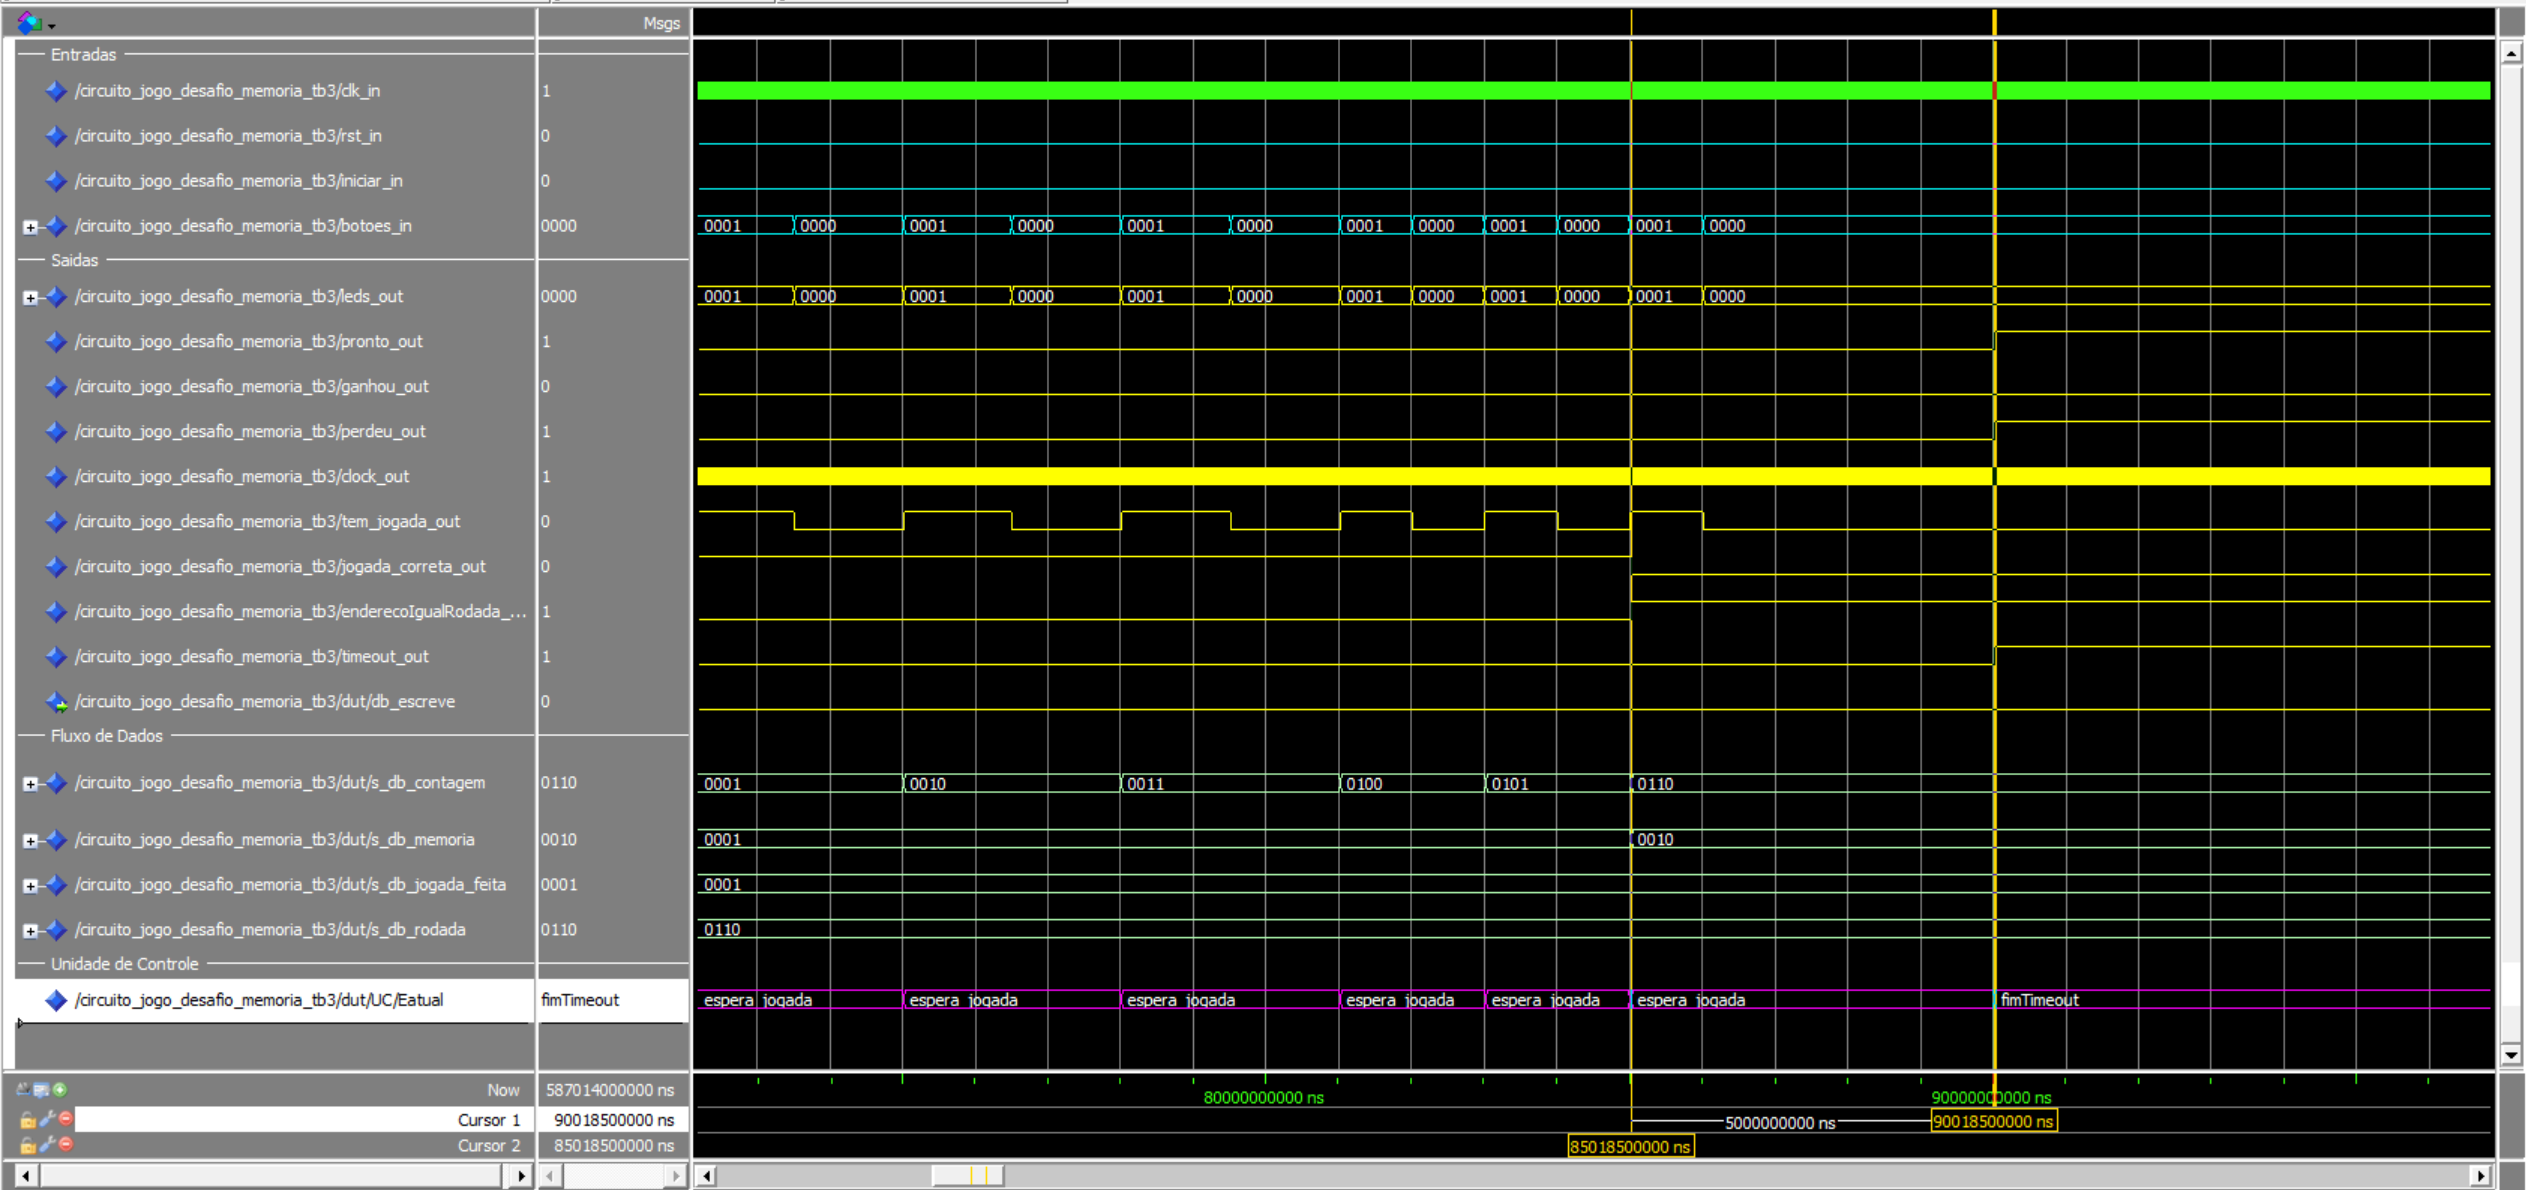
\includegraphics[scale=0.25]{Images/Semana 1/testbench1_0.png}
    \caption{Formas de onda da demonstração da escrita na memória e da realização de jogadas}
    \label{fig:testbench1_0}
\end{figure}

\begin{figure}[H]
    \centering
    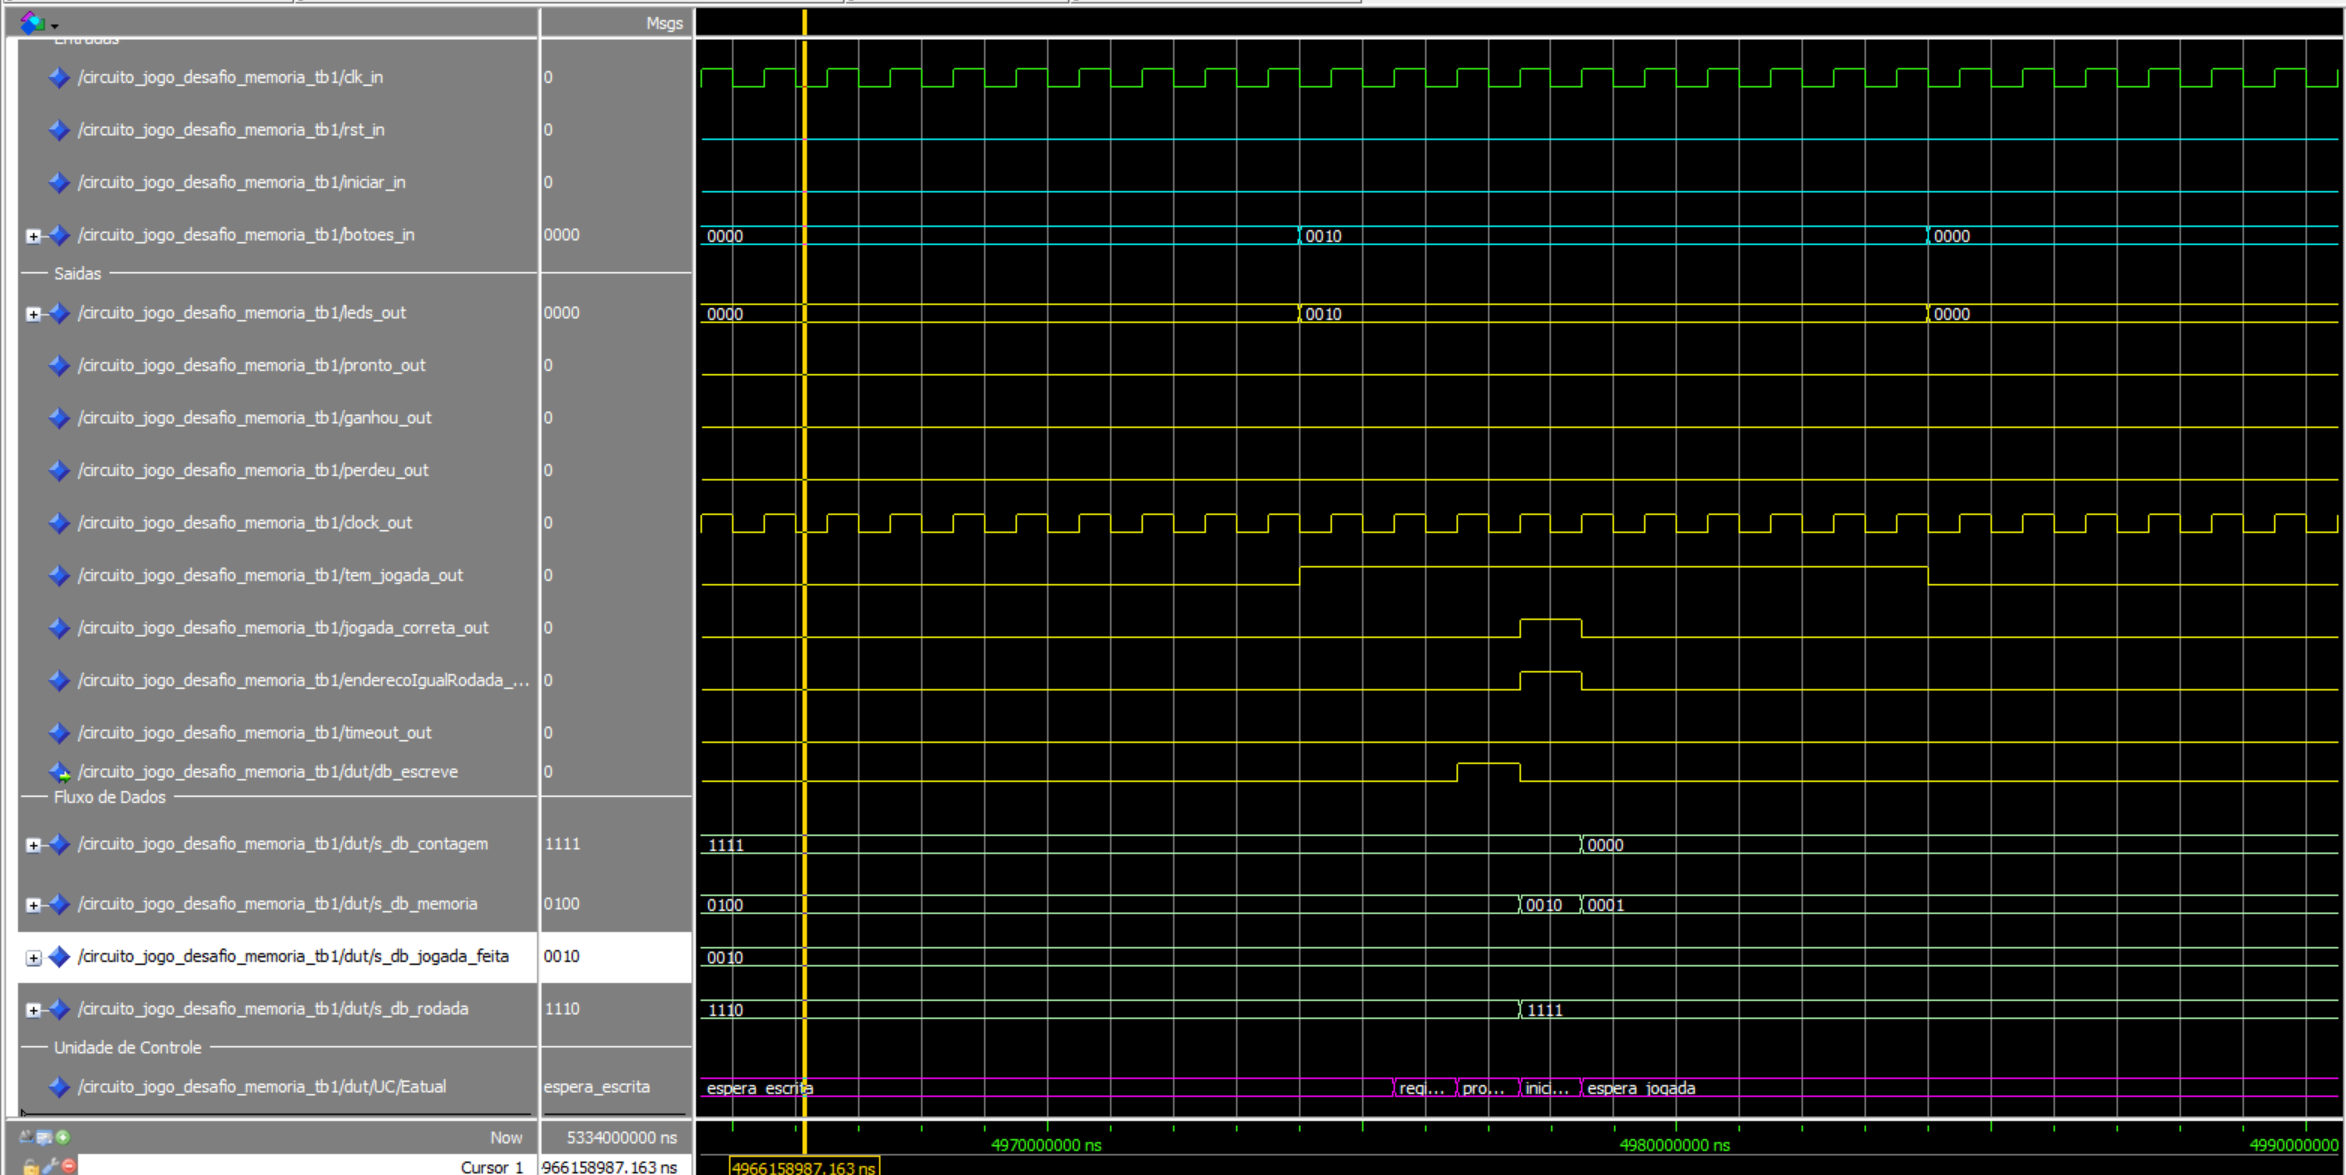
\includegraphics[scale=0.25]{Images/Semana 1/testbench1_1.png}
    \caption{Formas de onda da demonstração da escrita na memória e da realização de jogadas}
    \label{fig:testbench1_1}
\end{figure}

\begin{figure}[H]
    \centering
    \includegraphics[scale=0.25]{Images/Semana 1/testbench1_2.png}
    \caption{Formas de onda da demonstração da escrita na memória e da realização de jogadas}
    \label{fig:testbench1_2}
\end{figure}


As formas de onda da figura \ref{fig:testbench2} apresentam o resultado do cenário de teste 2.

\begin{figure}[H]
    \centering
    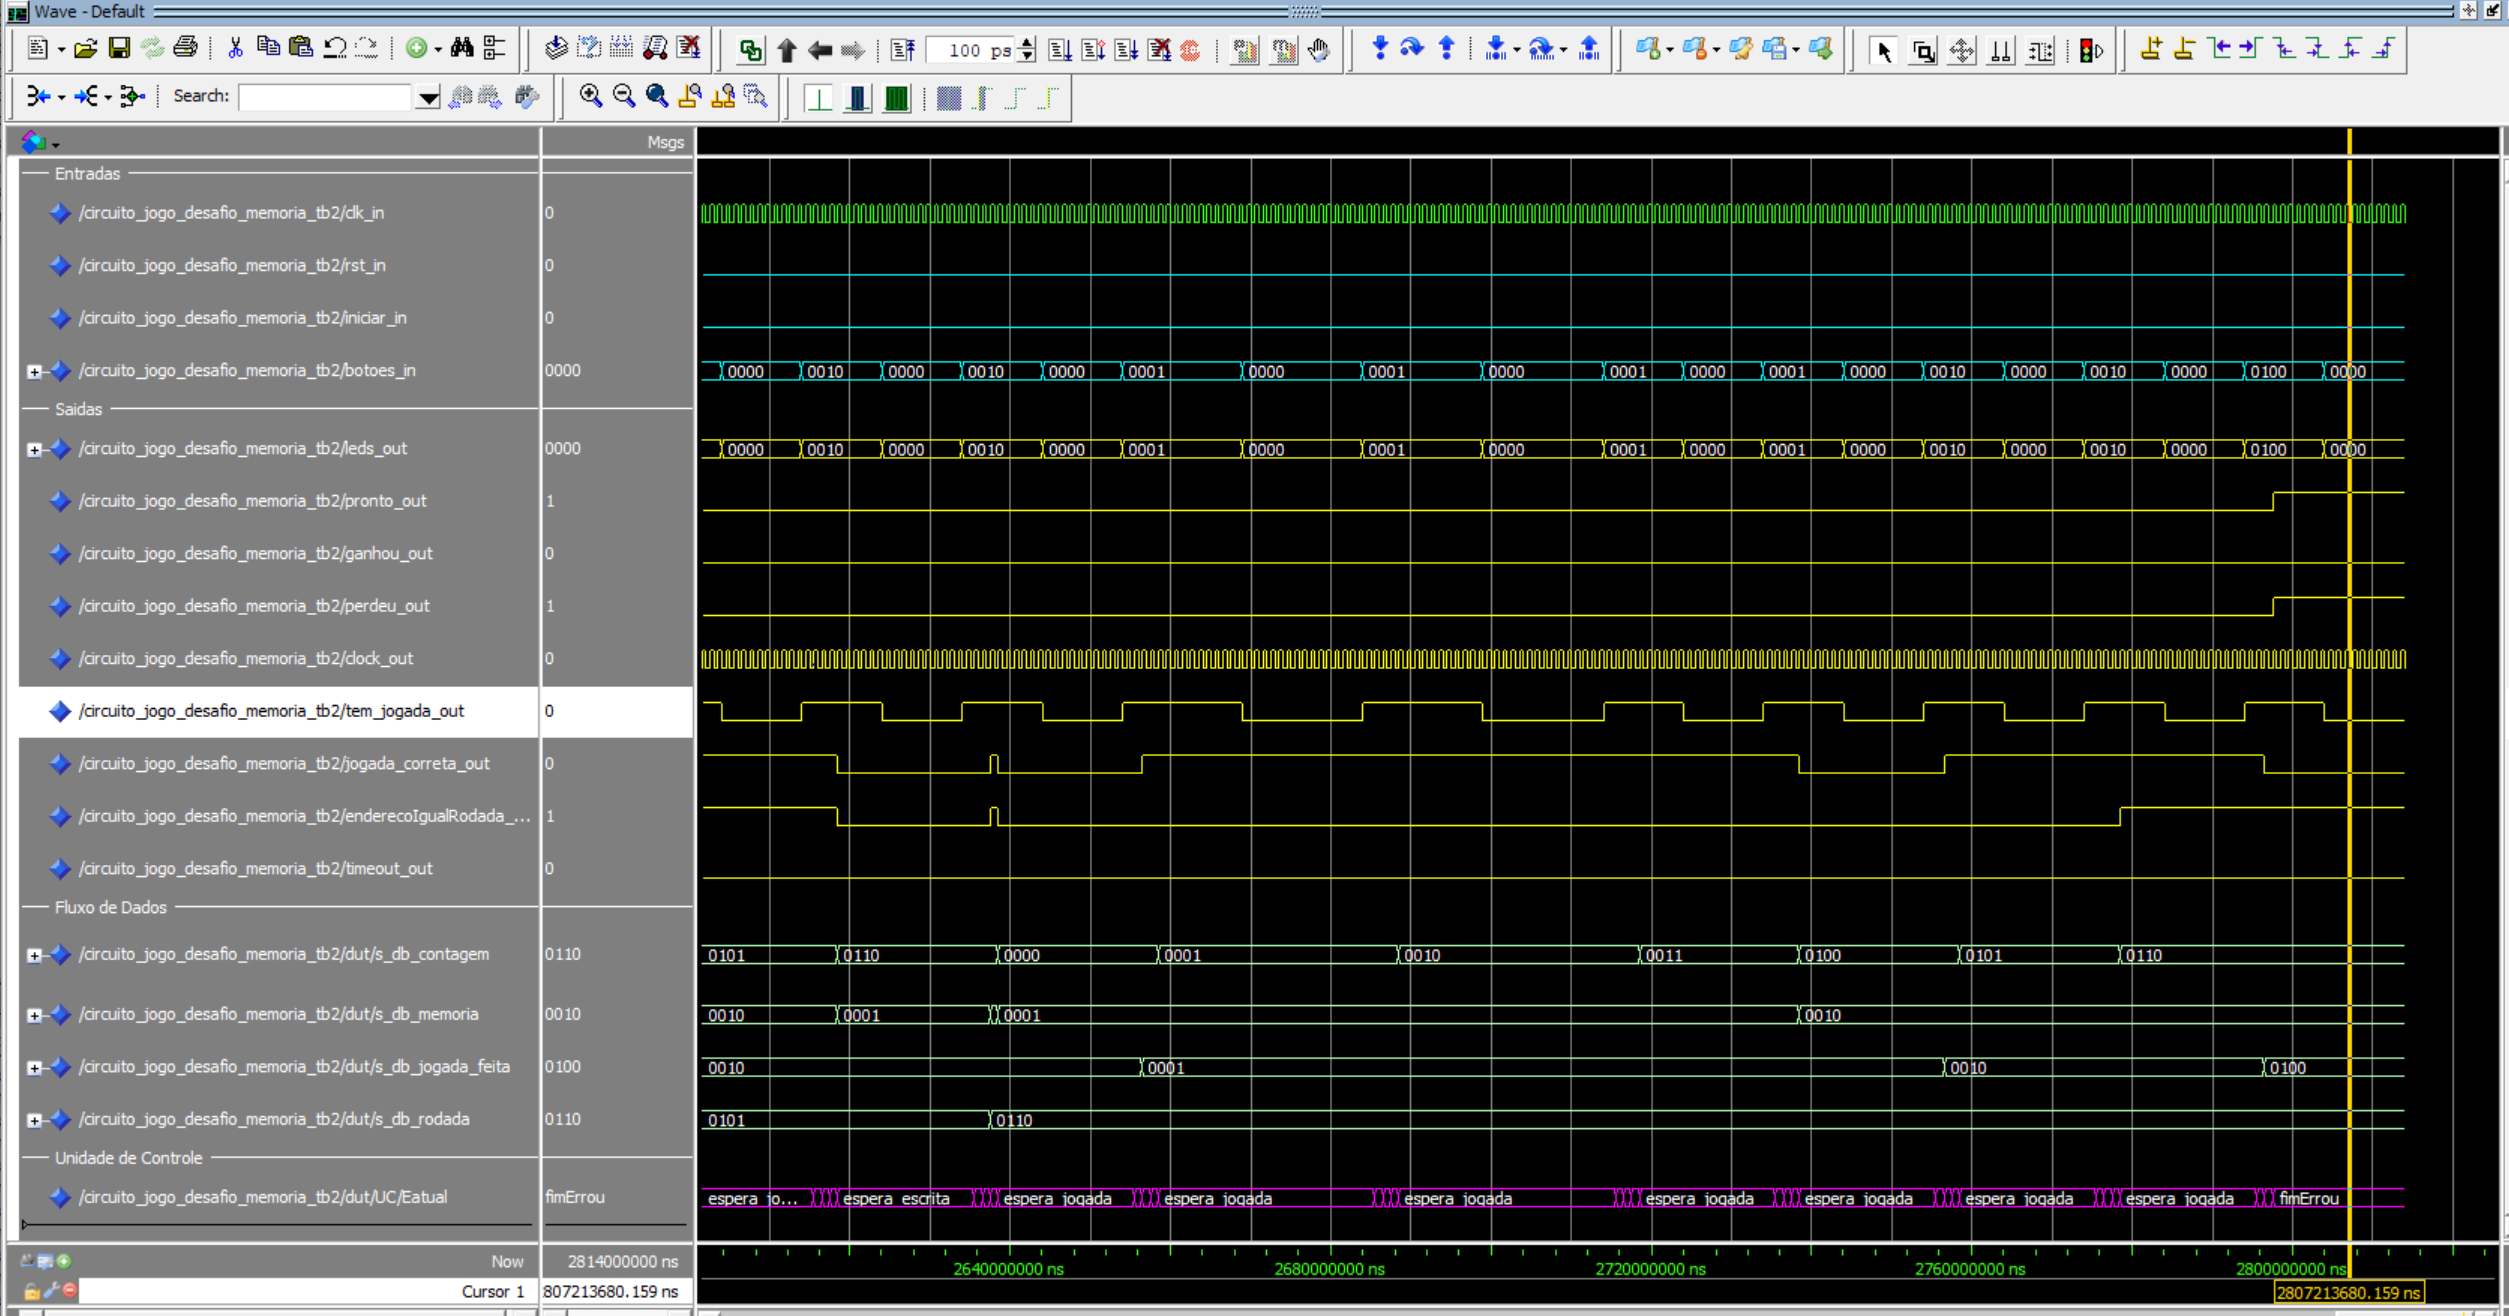
\includegraphics[scale=0.25]{Images/Semana 1/testbench2.png}
    \caption{Formas de onda da demonstração da escrita na memória e da realização de jogadas um bit por vez}
    \label{fig:testbench2}
\end{figure}

As formas de onda da figura \ref{fig:testbench3} apresentam o resultado do cenário de teste 3. Nota-se o incremento na contagem de erros a cada jogada errada cometida. Uma jogada errada é caracterizada pelo aperto de um botão que não deveria ter sido apertado.

\begin{figure}[H]
    \centering
    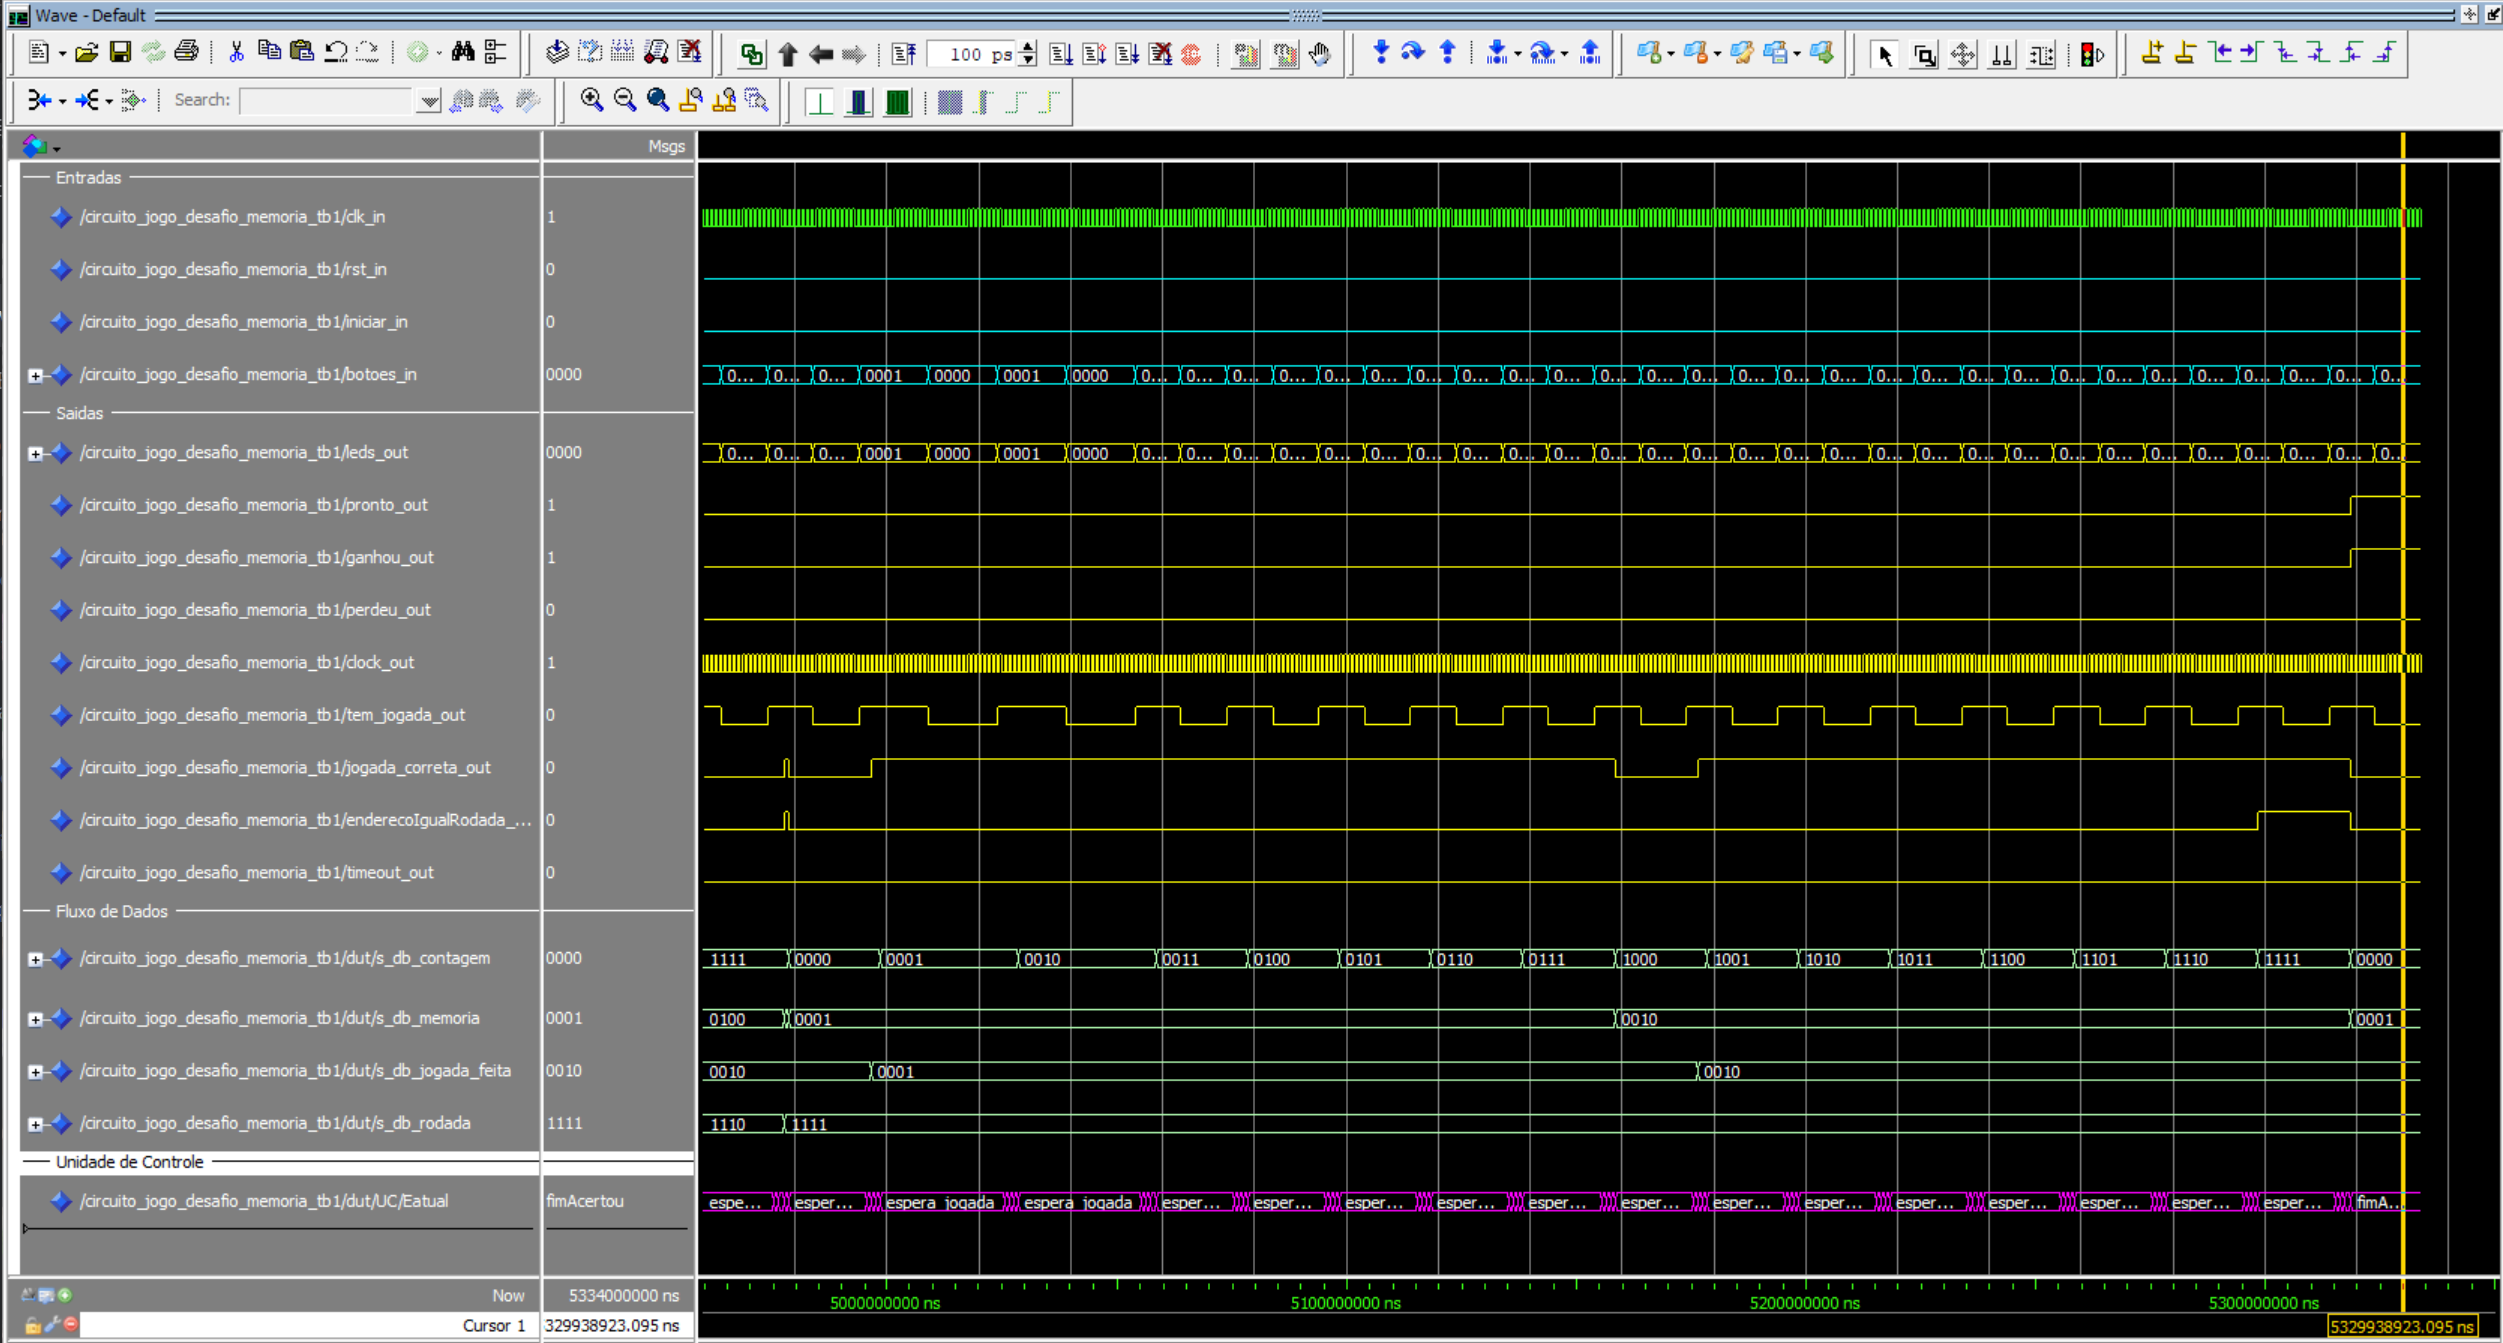
\includegraphics[scale=0.29]{Images/Semana 1/testbench3.png}
    \caption{Formas de onda da demonstração do erro em jogadas}
    \label{fig:testbench3}
\end{figure}

As formas de onda da figura \ref{fig:testbench4} apresentam o resultado do cenário de teste 4. Nota-se o incremento na contagem de erros a cada \textit{timeout} ocorrido. \textit{Timeouts} acontecem após 30 segundos de inatividade do jogador.

\begin{figure}[H]
    \centering
    \includegraphics[scale=0.265]{Images/Semana 1/testbench4.png}
    \caption{Formas de onda da demonstração da do \textit{timeout} em jogadas.}
    \label{fig:testbench4}
\end{figure}

Após os testes, pode-se concluir que o circuito desenvolvido funciona caso a mudança no valor dos botões se mantenha estável o suficiente durante as transições dos subestados \textit{espera\_jogada} e \textit{registra\_jogada}. Caso isso não ocorra, é possível que o valor armazenado durante o estado \textit{registra\_jogada} não condiza com o valor detectado durante o estado \textit{espera\_jogada}. Levando isso em conta, nota-se que os requisitos funcionais lógicos do circuito estão corretamente implementados em VHDL.


\subsection{Síntese do Circuito na Placa FPGA}
\label{subsec:sintese}

Tendo-se verificado logicamente o projeto, prosseguiu-se com a síntese do circuito para programação na FPGA DE0-CV (5CEBA4F23C7N). Alterou-se, então, a arquitetura do componente \textit{ram\_16x6}, do fluxo de dados, da arquitetura \textit{ram\_modelsim} (usada na simulação do circuito) para a arquitetura \textit{ram\_mif}, de modo a preencher os conteúdos da memória com dados especificados no arquivo de inicialização de memória \textit{ram\_conteudo\_jogadas.mif}, disponibilizado junto ao material da experiência anterior.

A figura \ref{fig:rtl} apresenta a visão \textit{Register Transfer Level} do circuito desenvolvido. Nas figuras \ref{fig:rtlDf1} e \ref{fig:rtlDf2}, ainda, é possível visualizar a visão RTL do Fluxo de Dados de maneira detalhada. A visão RTL apresentada é equivalente ao diagrama de blocos da figura \ref{fig:df}. 

Finalmente, pode-se visualizar as máquinas de estados geradas pelas codificações apresentadas na seção \ref{subsec:projetoVhdl1} através da ferramenta \textit{State Machine Viewer} nas figuras \ref{fig:sm} e \ref{fig:smSub}, assim como as transições de estados e seus sinais de condição nas tabelas \ref{fig:smTable} e \ref{fig:smSubTable}. Designou-se, então, os pinos internos e interfaceamento externo (GPIO) como especificado na tabela \ref{tab:pinagemFPGA1}. As entradas e saídas do circuito conectam-se ao dispositivo \textit{Analog Discovery}, que permite a visualização, geração e controle de sinais digitais e analógicos. No caso, o \textit{clock} será gerado como um sinal periódico de 1kHz  e o sinal \textit{dado\_escrita}, como um barramento de dados através do programa \textit{WaveForms} (configuração de \textit{Patterns} mostrada na figura \ref{fig:wfClock}), as outras entradas do circuito configuram-se como botões (\textit{StaticIO -- Button 0/1}) e algumas saídas, como LEDs (\textit{StaticIO -- LED}), como na figura \ref{fig:wv}.

\begin{figure}[H]
\centering
\includegraphics[scale=0.25]{Images/Semana 1/rtl.png} 
    \caption{Visão RTL do circuito}
    \label{fig:rtl}
\end{figure} 

\begin{figure}[H]
\centering
\includegraphics[scale=0.35]{Images/Semana 1/rtlDf1.png} 
    \caption{Visão RTL do Fluxo de Dados do circuito}
    \label{fig:rtlDf1}
\end{figure} 

\begin{figure}[H]
\centering
\includegraphics[scale=0.35]{Images/Semana 1/rtlDf2.png} 
    \caption{Visão RTL do Fluxo de Dados do circuito---continuação}
    \label{fig:rtlDf2}
\end{figure} 

\begin{figure}[H]
\centering
\includegraphics[scale=0.25]{Images/Semana 1/sm.png} 
    \caption{Visão SM da Unidade de Controle do circuito}
    \label{fig:sm}
\end{figure} 

\begin{figure}[H]
\centering
\includegraphics[scale=0.25]{Images/Semana 1/smSub.png} 
    \caption{Visão SM dos subestados da Unidade de Controle do circuito}
    \label{fig:smSub}
\end{figure} 

\begin{figure}[H]
\centering
\includegraphics[scale=0.5]{Images/Semana 1/smTable.png} 
    \caption{Tabela com as transições de estado da máquina de estados da figura \ref{fig:sm}.}
    \label{fig:smTable}
\end{figure} 

\begin{figure}[H]
\centering
\includegraphics[scale=0.5]{Images/Semana 1/smSubTable.png} 
    \caption{Tabela com as transições de estado da submáquina de estados da figura \ref{fig:smSub}.}
    \label{fig:smSubTable}
\end{figure} 



\begin{table}[H]
\centering
\scriptsize
\begin{tabular}{c|c|c|c|c|}
\cline{2-5}
\multicolumn{1}{l|}{\textbf{}}                   & Sinal                   & Pino na Placa DE0-CV & Pino no FPGA                                                                                                                                                                          & Analog Discovery               \\ \hline
\multicolumn{1}{|c|}{\multirow{15}{*}{entradas}} & CLOCK                   & GPIO\_0\_D0          & PIN\_N16                                                                                                                                                                              & Patterns – Clock – 1 KHz – DIO0 \\ \cline{2-5} 
\multicolumn{1}{|c|}{}                           & RESET                   & GPIO\_0\_D1          & PIN\_B16                                                                                                                                                                              & StaticIO – Button 0/1 – DIO1          \\ \cline{2-5} 
\multicolumn{1}{|c|}{}                           & INICIAR                 & GPIO\_0\_D3          & PIN\_C16                                                                                                                                                                              & StaticIO – Button 0/1 – DIO2          \\ \cline{2-5} 
\multicolumn{1}{|c|}{}                           & BOTOES(0)               & GPIO\_0\_D11         & PIN\_R22                                                                                                                                                                              & \multicolumn{1}{l|}{}          \\ \cline{2-5} 
\multicolumn{1}{|c|}{}                           & BOTOES(1)               & GPIO\_0\_D13         & PIN\_T22                                                                                                                                                                              & \multicolumn{1}{l|}{}          \\ \cline{2-5} 
\multicolumn{1}{|c|}{}                           & BOTOES(2)               & GPIO\_0\_D15         & PIN\_N19                                                                                                                                                                              & \multicolumn{1}{l|}{}          \\ \cline{2-5} 
\multicolumn{1}{|c|}{}                           & BOTOES(3)               & GPIO\_0\_D17         & PIN\_P19                                                                                                                                                                              & \multicolumn{1}{l|}{}          \\ \cline{2-5} 
\multicolumn{1}{|c|}{}                           & BOTOES(4)               & GPIO\_0\_D19         & PIN\_P17                                                                                                                                                                              &                                \\ \cline{2-5} 
\multicolumn{1}{|c|}{}                           & BOTOES(5)               & GPIO\_0\_D21         & PIN\_M18                                                                                                                                                                              &                                \\ \cline{2-5} 
\multicolumn{1}{|c|}{}                           & DADO\_ESCRITA(0)        & GPIO\_0\_D10         & PIN\_N21                                                                                                                                                                              &  Patterns – BUS – DIO10 \\ \cline{2-5} 
\multicolumn{1}{|c|}{}                           & DADO\_ESCRITA(1)        & GPIO\_0\_D12         & PIN\_R21                                                                                                                                                                              &  Patterns – BUS – DIO11 \\ \cline{2-5} 
\multicolumn{1}{|c|}{}                           & DADO\_ESCRITA(2)        & GPIO\_0\_D14         & PIN\_N20                                                                                                                                                                              &  Patterns – BUS – DIO12    \\ \cline{2-5} 
\multicolumn{1}{|c|}{}                           & DADO\_ESCRITA(3)        & GPIO\_0\_D16         & PIN\_M22                                                                                                                                                                              &  Patterns – BUS – DIO13 \\ \cline{2-5} 
\multicolumn{1}{|c|}{}                           & DADO\_ESCRITA(4)        & GPIO\_0\_D18         & PIN\_L22                                                                                                                                                                              &  Patterns – BUS – DIO14 \\ \cline{2-5} 
\multicolumn{1}{|c|}{}                           & DADO\_ESCRITA(5)        & GPIO\_0\_D20         & PIN\_P16                                                                                                                                                                              &  Patterns – BUS – DIO15 \\ \hline
\multicolumn{1}{|c|}{\multirow{2}{*}{saídas}}    & FIMDEJOGO               & GPIO\_1\_D11         & PIN\_J18                                                                                                                                                                              & StaticIO – LED – DIO8          \\ \cline{2-5} 
\multicolumn{1}{|c|}{}                           & ERROS                   & HEX1 e HEX0          & \thead{PIN\_U21 \\ PIN\_U21 \\ PIN\_W22 \\ PIN\_W21 \\ PIN\_Y22 \\ PIN\_Y21 \\ PIN\_AA22 \\ PIN\_AA20 \\ PIN\_AB20 \\ PIN\_AA19 \\ PIN\_AA18 \\ PIN\_AB18 \\ PIN\_AA17 \\ PIN\_U22}   &                                \\ \hline
\multicolumn{1}{|c|}{\multirow{8}{*}{depuração}} & db\_clock               & GPIO\_0\_D23         & PIN\_L17                                                                                                                                                                              & StaticIO – LED – DIO3          \\ \cline{2-5} 
\multicolumn{1}{|c|}{}                           & db\_tem\_jogada         & GPIO\_0\_D25         & PIN\_K17                                                                                                                                                                              & StaticIO – LED – DIO4          \\ \cline{2-5} 
\multicolumn{1}{|c|}{}                           & db\_enderecoIgualRodada & GPIO\_0\_D27         & PIN\_P18                                                                                                                                                                              & StaticIO – LED – DIO9          \\ \cline{2-5} 
\multicolumn{1}{|c|}{}                           & db\_contagem            & LEDR9 a LEDR6        & \thead{PIN\_U2\\ PIN\_U1\\ PIN\_L2\\ PIN\_L1}                                                                                                                                         & \multicolumn{1}{l|}{}          \\ \cline{2-5} 
\multicolumn{1}{|c|}{}                           & db\_memoria             & HEX3 e HEX2          & \thead{PIN\_Y19 \\ PIN\_AB17 \\ PIN\_AA10 \\  PIN\_Y14 \\ PIN\_V14 \\  PIN\_AB22 \\  PIN\_AB21 \\PIN\_Y16 \\ PIN\_W16 \\ PIN\_Y17 \\ PIN\_V16 \\ PIN\_U17 \\ PIN\_V18 \\ PIN\_V19 \\} & \multicolumn{1}{l|}{}          \\ \cline{2-5} 
\multicolumn{1}{|c|}{}                           & db\_jogada\_feita       & LEDR5 a LEDR0        & \thead{PIN\_AA2\\ PIN\_AA1\\ PIN\_W2\\ PIN\_Y3\\ PIN\_N2\\ PIN\_N1}                                                                                                                   & \multicolumn{1}{l|}{}          \\ \cline{2-5} 
\multicolumn{1}{|c|}{}                           & db\_rodada              & Display HEX4         & \thead{PIN\_U20\\ PIN\_Y20\\ PIN\_V20\\ PIN\_U16\\ PIN\_U15\\ PIN\_Y15\\ PIN\_P9}                                                                                                     & \multicolumn{1}{l|}{}          \\ \cline{2-5} 
\multicolumn{1}{|c|}{}                           & db\_estado              & Display HEX5 & \thead{PIN\_N9 \\ PIN\_M8 \\ PIN\_T14 \\  PIN\_P14 \\  PIN\_C1 \\ PIN\_C2 \\ PIN\_W19}                                                                       & \multicolumn{1}{l|}{}          \\ \hline
\end{tabular}
\caption{Pinagem do projeto}
\label{tab:pinagemFPGA1}
\end{table}

\begin{figure}[H]
\centering
\includegraphics[scale=0.45]{Images/Semana 1/pinPlanner1.png} 
    \caption{Designação de pinos através da ferramenta \textit{Pin Planner}}
    \label{fig:pinPlanner1}
\end{figure} 

\begin{figure}[H]
\centering
\includegraphics[scale=0.45]{Images/Semana 1/pinPlanner2.png} 
    \caption{Designação de pinos através da ferramenta \textit{Pin Planner}}
    \label{fig:pinPlanner2}
\end{figure} 

\begin{figure}[H]
\centering
\includegraphics[scale=0.45]{Images/Semana 1/pinPlanner3.png} 
    \caption{Designação de pinos através da ferramenta \textit{Pin Planner}}
    \label{fig:pinPlanner3}
\end{figure} 

\begin{figure}[H]
\centering
\includegraphics[scale=0.25]{Images/Semana 1/WaveFormsClock.png} 
    \caption{Configuração do \textit{clock} e do barramento de dados para o sinal \textit{dado\_escrita}, na \textit{Analog Discovery}}
    \label{fig:wfClock}
\end{figure} 

\begin{figure}[H]
\centering
\includegraphics[scale=0.25]{Images/Semana 1/wv.png} 
    \caption{Configuração da ligação entre a FPGA e a \textit{Analog Discovery}, incluindo \textit{LED}s e \textit{Buttons}}
    \label{fig:wv}
\end{figure}

\section{Planejamento de Aula Prática}

Durante a aula prática, prossegue-se para a programação da FPGA da placa de desenvolvimento DE0-CV e a execução dos testes das tabelas \ref{tab:testbench1_exp}, \ref{tab:testbench2_exp}, \ref{tab:testbench3_exp} e \ref{tab:testbench4_exp}, inseridas previamente na seção \ref{sec:exp} com a coluna \textbf{Resultado Observado} a preencher. Primeiramente, programa-se a FPGA com o circuito desenvolvido, sintetizado e cujas pinagens refletem a tabela \ref{tab:pinagemFPGA1}. Para tanto, é necessário conectar a DE0-CV ao computador por USB, abrir o programa \textit{Quartus}, através do qual realizou-se a pinagem como descrito na seção \ref{subsec:sintese}, e programar a DE0-CV através da funcionalidade \textit{Programmer}. 

Depois, desliga-se a FPGA para fazer as ligações com o \textit{Analog Discovery}. Inicialmente liga-se o terra ao pino GPIO\_0\_12 e GPIO\_1\_12 da DE0-CV, como especificado na figura \ref{fig:analogdiscovery}, que mostra o diagrama \textit{pinout} do \textit{Analog Discovery}, e na figura \ref{fig:gpio}, que mostra a pinagem da placa DE0-CV. Prossegue-se com a montagem da matriz de botões, como na figura \ref{fig:botoes3x2}.

\begin{figure}[H]
\centering
\includegraphics[scale=0.25]{Images/Semana 1/botoes3x2.png} 
    \caption{Montagem da matriz de botões 3x2}
    \label{fig:botoes3x2}
\end{figure}


A seguir, conectam-se os pinos de entrada e saída mapeados ao circuito na FPGA como especificado na tabela \ref{tab:pinagemFPGA1} e explicitado pelas imagens \ref{fig:analogdiscovery} e \ref{fig:gpio}.

Tendo todas as conexões realizadas, passa-se a utilizar o software \textit{WaveForms} para operar os sinais do circuito. Nota-se que, diferentemente dos demais, os sinais de \textit{clock} e \textit{dado\_escrita} são configurados dentro do \textit{WaveForms} utilizando-se sua ferramenta \textit{Patterns} como uma onda retangular com frequência de 1kHz e um barramento de dados. Os demais sinais são configurados como \textit{StaticIO -- Button 0/1} (entradas) ou \textit{StaticIO -- LED} (saídas), como na figura \ref{fig:wv}.

Ressalta-se que pode-se alterar os nomes dos sinais do WaveForms para condizerem com os nomes especificados na tabela da pinagem \ref{tab:pinagemFPGA1}, utilizando a funcionalidade de \textit{View} do programa, como na figura \ref{fig:wv}.

Enfim, testa-se o circuito a fim de averiguar sua correta funcionalidade. A lista abaixo resume brevemente as tarefas a serem executadas.

\begin{enumerate}
    \item Conexão dos pinos do dispositivo \textit{Analog Discovery} como especificado na tabela \ref{tab:pinagemFPGA1}, com auxílio dos diagramas \ref{fig:analogdiscovery} e \ref{fig:gpio};
    \item Programação da FPGA com o circuito desenvolvido (designação de pinos já realizada através da ferramenta \textit{Pin Planner}, do \textit{Quartus}, como especificado na tabela \ref{tab:pinagemFPGA1});
    \item Teste do circuito através do software \textit{WaveForms} e dos botões (figura \ref{fig:botoes3x2}), e preenchimento dos resultados de acordo com as tabelas \ref{tab:testbench1_exp}, \ref{tab:testbench2_exp}, \ref{tab:testbench3_exp} e \ref{tab:testbench4_exp} previamente inseridas no documento na seção \ref{sec:exp} a fim de acelerar o processo de teste e relato de resultados;
\end{enumerate}

\subsection{Depuração}
\label{subsec:depuracao}

Há a possibilidade de que o circuito não funcione como o esperado. Por isso, é fundamental mapear o processo de depuração aos sinais de depuração apresentados na seção \ref{subsec:projetoLogico1}. Pode-se, identificar algumas possíveis causas mais prováveis de erros no circuito. 

Uma fonte de erro significativa são os sinais de entrada da placa DE0-CV. Assim, é fundamental certificar-se os seguintes aspectos.

\begin{enumerate}
    \item De que o terra esta propriamente conectado na placa DE0-CV, pois, caso contrário, o circuito não conseguirá interpretar os sinais que recebe corretamente.
   \item De que a placa recebe o sinal de \textit{clock}. Isso pode ser feito verificando-se o \textit{LEDR0} da placa, pois o sinal \textit{db\_clock} está mapeado ao LED. Vale ressaltar que, devido a alta frequência do sinal (1kHz) o LED não aparentará alternar-se entre ligado e desligado, mantendo-se em nível alto. Pode ser interessante diminuir a frequência do sinal no \textit{Waveforms} para que a correta observação do sinal possa ser realizada.
   \item Se existe algum mau contato nos fios. É comum que, ao manipular-se os fios, alguma interferência afete a transmissão dos sinais entre a \textit{Analog Discovey} e a FPGA. Modificar o posicionamento dos dispositivos geralmente é suficiente para resolver esse tipo de problema. 
   \item Se a conexão entre o dispositivo \textit{Analog Discovery} foi realizada de maneira correta. Há a possibilidade de que as ligações entre as GPIOs e o \textit{Analog Discovery} não tenham sido realizadas corrretamente.
   \item De que os sinais de depuração do circuito (prefixados por \textit{db\_}) condizem com o que especificou-se na tabela \ref{tab:pinagemFPGA1} através das simulações da seção \ref{subsubsec:tbVhdl1}. Em particular, o sinal de depuração \textit{db\_jogada\_feita} permite a verificação da conexão da entrada \textit{botoes}. Ademais, \textit{db\_enderecoIgualRodada} permite a aferição da comparação entre as saídas dos contadores \textit{ContEnd} e \textit{ContRod} e \textit{db\_estado}, do estado interno da unidade de controle a qualquer momento.
\end{enumerate}

Há também a possibilidade do circuito não ter sido sintetizado de maneira correta na DE0-CV. Pode-se, então, programá-la novamente, certificando de que as pinagens especificadas na tabela \ref{tab:pinagemFPGA1} foram realizadas de maneira correta.

\section{Atividades Experimentais}
\label{sec:exp}

Durante as atividades experimentais, percebeu-se que a montagem da figura \ref{fig:botoes3x2} não funcionaria na experiência. Isso se deve ao fato de que não há resistor de \textit{pull-up}, nem de \textit{pull-down} na entrada da FPGA. Portanto, montou-se o circuito com resistores de \textit{pull-up} como na figura \ref{fig:protoboard1} abaixo:

\begin{figure}[H]
\centering
\includegraphics[scale=0.25]{Images/Semana 1/protoboard1.jpg} 
    \caption{\textit{Protoboard} com botões. Os botões comprados são grandes demais para a \textit{protoboard}, o que impossibilita a montagem da matriz 3x2. Nas próximas experiências, essa característica sera corrigida.}
    \label{fig:protoboard1}
\end{figure}

Após a ligação dos componentes no \textit{protoboard} como acima, conectaram-se os aparelhos de acordo com a tabela \ref{tab:pinagemFPGA1}, com auxílio dos diagramas \ref{annex:analogDiscovery} e \ref{annex:gpio}. A montagem se encontra na figura \ref{fig:montagem1}, como abaixo:

\begin{figure}[H]
\centering
\includegraphics[scale=0.09]{Images/Semana 1/montagem1.jpg} 
    \caption{\textit{Protoboard} com botões. Os botões comprados são grandes demais para a \textit{protoboard}, o que impossibilita a montagem da matriz 3x2. Nas próximas experiências, essa característica sera corrigida.}
    \label{fig:montagem1}
\end{figure}

Além disso, dado que montou-se o circuito com resistores de \textit{pull-up}, foi necessário a alteração do código do componente \textit{braille\_teacher} de modo a garantir o correto funcionamento do circuito, invertendo-se o sinal de entrada, como na figura \ref{fig:modificacoes} abaixo:

\begin{figure}[H]
\centering
\includegraphics[scale=0.5]{Images/Semana 1/modificacoes.png} 
    \caption{Modificações do código VHDL do componente \textit{braille\_teacher}.}
    \label{fig:modificacoes}
\end{figure}


Em seguida, prosseguiu-se para o teste do circuito pelos cenários de teste das tabelas \ref{tab:testbench1_exp}, \ref{tab:testbench2_exp}, \ref{tab:testbench3_exp} e \ref{tab:testbench4_exp}.


\begin{table}[H]
\centering
\begin{tabular}{|cccc|}
\hline
\multicolumn{4}{|c|}{\textbf{Cenário 1 --- Jogador acerta todas as jogadas}}                                                                                                                                                \\ \hline
\multicolumn{1}{|c|}{\textbf{\#}} & \multicolumn{1}{c|}{\textbf{Operação}}   & \multicolumn{1}{c|}{\textbf{Sinais de Entrada}}                                         & \multicolumn{1}{c|}{\textbf{Resultado Observado}}   \\ \hline
\multicolumn{1}{|c|}{c.i}         & \multicolumn{1}{c|}{Condições Iniciais}  & \multicolumn{1}{l|}{}                                                                   &                                                    \\ \hline
\multicolumn{1}{|c|}{1}           & \multicolumn{1}{c|}{Resetar o circuito}  & \multicolumn{1}{c|}{reset=1}                                                            &                                                    \\ \hline
\multicolumn{1}{|c|}{2}           & \multicolumn{1}{c|}{Inicia o circuito}   & \multicolumn{1}{c|}{iniciar=1}                                                            &                                                    \\ \hline
\multicolumn{1}{|c|}{3}           & \multicolumn{1}{c|}{Faz a rodada 1}      & \multicolumn{1}{c|}{\thead{dado\_escrita="100000" e botoes="100000"}}                           & \thead{erros=0x0\\ db\_jogada\_feita="100000"              }\\ \hline
\multicolumn{1}{|c|}{4}           & \multicolumn{1}{c|}{Faz a rodada 2}      & \multicolumn{1}{c|}{\thead{dado\_escrita="101000"\\ repete botoes anteriores e botoes="101000"}} & \thead{erros=0x0\\ db\_jogada\_feita="101000"}              \\ \hline
\multicolumn{1}{|c|}{5}           & \multicolumn{1}{c|}{Faz a rodada 3}      & \multicolumn{1}{c|}{\thead{dado\_escrita="110000"\\ repete botoes anteriores e botoes="110000"}} & \thead{erros=0x0\\ db\_jogada\_feita="110000"}              \\ \hline
\multicolumn{1}{|c|}{6}           & \multicolumn{1}{c|}{Faz a rodada 4}      & \multicolumn{1}{c|}{\thead{dado\_escrita="110100"\\ repete botoes anteriores e botoes="110100"}} & \thead{erros=0x0\\ db\_jogada\_feita="110100"}              \\ \hline
\multicolumn{1}{|c|}{7}           & \multicolumn{1}{c|}{Faz a rodada 5}      & \multicolumn{1}{c|}{\thead{dado\_escrita="100100"\\ repete botoes anteriores e botoes="100100"}} & \thead{erros=0x0\\ db\_jogada\_feita="100100"}              \\ \hline
\multicolumn{1}{|c|}{8}           & \multicolumn{1}{c|}{Faz a rodada 6}      & \multicolumn{1}{c|}{\thead{dado\_escrita="111000"\\ repete botoes anteriores e botoes="111000"}} & \thead{erros=0x0\\ db\_jogada\_feita="111000"}              \\ \hline
\multicolumn{1}{|c|}{9}          & \multicolumn{1}{c|}{Faz a rodada 7}      & \multicolumn{1}{c|}{\thead{dado\_escrita="111100"\\ repete botoes anteriores e botoes="111100"}} & \thead{erros=0x0\\ db\_jogada\_feita="111100"}              \\ \hline
\multicolumn{1}{|c|}{10}          & \multicolumn{1}{c|}{Faz a rodada 8}      & \multicolumn{1}{c|}{\thead{dado\_escrita="101100"\\ repete botoes anteriores e botoes="101100"}} & \thead{erros=0x0\\ db\_jogada\_feita="101100"}              \\ \hline
\multicolumn{1}{|c|}{11}          & \multicolumn{1}{c|}{Faz a rodada 9}      & \multicolumn{1}{c|}{\thead{dado\_escrita="011000"\\ repete botoes anteriores e botoes="011000"}} & \thead{erros=0x0\\ db\_jogada\_feita="011000"}              \\ \hline
\multicolumn{1}{|c|}{12}          & \multicolumn{1}{c|}{Faz a rodada 10}     & \multicolumn{1}{c|}{\thead{dado\_escrita="011100"\\ repete botoes anteriores e botoes="011100"}} & \thead{erros=0x0\\ db\_jogada\_feita="011100"}              \\ \hline
\multicolumn{1}{|c|}{13}          & \multicolumn{1}{c|}{Faz a rodada 11}     & \multicolumn{1}{c|}{\thead{dado\_escrita="100010"\\ repete botoes anteriores e botoes="100010"}} & \thead{erros=0x0\\ db\_jogada\_feita="100010"}              \\ \hline
\multicolumn{1}{|c|}{14}          & \multicolumn{1}{c|}{Faz a rodada 12}     & \multicolumn{1}{c|}{\thead{dado\_escrita="101010"\\ repete botoes anteriores e botoes="101010"}} & \thead{erros=0x0\\ db\_jogada\_feita="101010"}              \\ \hline
\multicolumn{1}{|c|}{15}          & \multicolumn{1}{c|}{Faz a rodada 13}     & \multicolumn{1}{c|}{\thead{dado\_escrita="110010"\\ repete botoes anteriores e botoes="110010"}} & \thead{erros=0x0\\ db\_jogada\_feita="110010"}              \\ \hline
\multicolumn{1}{|c|}{16}          & \multicolumn{1}{c|}{Faz a rodada 14}     & \multicolumn{1}{c|}{\thead{dado\_escrita="110110"\\ repete botoes anteriores e botoes="110110"}} & \thead{erros=0x0\\ db\_jogada\_feita="110110"}              \\ \hline
\multicolumn{1}{|c|}{17}          & \multicolumn{1}{c|}{Faz a rodada 15}     & \multicolumn{1}{c|}{\thead{dado\_escrita="100110"\\ repete botoes anteriores e botoes="100110"}} & \thead{erros=0x0\\ db\_jogada\_feita="100110"}              \\ \hline
\multicolumn{1}{|c|}{18}          & \multicolumn{1}{c|}{Faz a rodada 16}     & \multicolumn{1}{c|}{\thead{dado\_escrita="111010"\\ repete botoes anteriores e botoes="111010"}} & \thead{erros=0x0\\ db\_jogada\_feita="111010"\\ fimDeJogo=1} \\ \hline
\multicolumn{1}{|c|}{19}          & \multicolumn{1}{c|}{Reinicia o circuito} & \multicolumn{1}{c|}{reset=1}                                                            & \multicolumn{1}{c|}{db\_estado=0x0}              \\ \hline
\multicolumn{1}{|c|}{20}          & \multicolumn{1}{c|}{Inicia o circuito}       & \multicolumn{1}{c|}{iniciar=1}                                                          &                                                    \\ \hline
\end{tabular}
\caption{Teste para o caso em que o jogador acerta todas as rodadas feitas.}
\label{tab:testbench1_exp}
\end{table}

\begin{table}[H]
\centering
\begin{tabular}{|cccc|}
\hline
\multicolumn{4}{|c|}{\textbf{Cenário 2 --- Jogador acerta todas as jogadas apertando um botão de cada vez}}                                                                                                                                                \\ \hline
\multicolumn{1}{|c|}{\textbf{\#}} & \multicolumn{1}{c|}{\textbf{Operação}}   & \multicolumn{1}{c|}{\textbf{Sinais de Entrada}}                                         & \multicolumn{1}{c|}{\textbf{Resultado Observado}}   \\ \hline
\multicolumn{1}{|c|}{c.i}         & \multicolumn{1}{c|}{Condições Iniciais}  & \multicolumn{1}{l|}{}                                                                   &                                                    \\ \hline
\multicolumn{1}{|c|}{1}           & \multicolumn{1}{c|}{Resetar o circuito}  & \multicolumn{1}{c|}{reset=1}                                                            &                                                    \\ \hline
\multicolumn{1}{|c|}{2}           & \multicolumn{1}{c|}{Inicia o circuito}   & \multicolumn{1}{c|}{iniciar=1}                                                            &                                                    \\ \hline
\multicolumn{1}{|c|}{3}           & \multicolumn{1}{c|}{Faz a rodada 1}      & \multicolumn{1}{c|}{\thead{dado\_escrita="100000" e botoes="100000"\\ um de cada vez}}                           & \thead{erros=0x0\\ db\_jogada\_feita="100000"              }\\ \hline
\multicolumn{1}{|c|}{4}           & \multicolumn{1}{c|}{Faz a rodada 2}      & \multicolumn{1}{c|}{\thead{dado\_escrita="101000"\\ repete botoes anteriores e botoes="101000"\\ um de cada vez}} & \thead{erros=0x0\\ db\_jogada\_feita="101000"}              \\ \hline
\multicolumn{1}{|c|}{5}           & \multicolumn{1}{c|}{Faz a rodada 3}      & \multicolumn{1}{c|}{\thead{dado\_escrita="110000"\\ repete botoes anteriores e botoes="110000"\\ um de cada vez}} & \thead{erros=0x0\\ db\_jogada\_feita="110000"}              \\ \hline
\multicolumn{1}{|c|}{6}           & \multicolumn{1}{c|}{Faz a rodada 4}      & \multicolumn{1}{c|}{\thead{dado\_escrita="110100"\\ repete botoes anteriores e botoes="110100"\\ um de cada vez}} & \thead{erros=0x0\\ db\_jogada\_feita="110100"}              \\ \hline
\multicolumn{1}{|c|}{7}           & \multicolumn{1}{c|}{Faz a rodada 5}      & \multicolumn{1}{c|}{\thead{dado\_escrita="100100"\\ repete botoes anteriores e botoes="100100"\\ um de cada vez}} & \thead{erros=0x0\\ db\_jogada\_feita="100100"}              \\ \hline
\multicolumn{1}{|c|}{8}           & \multicolumn{1}{c|}{Faz a rodada 6}      & \multicolumn{1}{c|}{\thead{dado\_escrita="111000"\\ repete botoes anteriores e botoes="111000"\\ um de cada vez}} & \thead{erros=0x0\\ db\_jogada\_feita="111000"}              \\ \hline
\multicolumn{1}{|c|}{9}          & \multicolumn{1}{c|}{Faz a rodada 7}      & \multicolumn{1}{c|}{\thead{dado\_escrita="111100"\\ repete botoes anteriores e botoes="111100"\\ um de cada vez}} & \thead{erros=0x0\\ db\_jogada\_feita="111100"}              \\ \hline
\multicolumn{1}{|c|}{10}          & \multicolumn{1}{c|}{Faz a rodada 8}      & \multicolumn{1}{c|}{\thead{dado\_escrita="101100"\\ repete botoes anteriores e botoes="101100"\\ um de cada vez}} & \thead{erros=0x0\\ db\_jogada\_feita="101100"}              \\ \hline
\multicolumn{1}{|c|}{11}          & \multicolumn{1}{c|}{Faz a rodada 9}      & \multicolumn{1}{c|}{\thead{dado\_escrita="011000"\\ repete botoes anteriores e botoes="011000"\\ um de cada vez}} & \thead{erros=0x0\\ db\_jogada\_feita="011000"}              \\ \hline
\multicolumn{1}{|c|}{12}          & \multicolumn{1}{c|}{Faz a rodada 10}     & \multicolumn{1}{c|}{\thead{dado\_escrita="011100"\\ repete botoes anteriores e botoes="011100"\\ um de cada vez}} & \thead{erros=0x0\\ db\_jogada\_feita="011100"}              \\ \hline
\multicolumn{1}{|c|}{13}          & \multicolumn{1}{c|}{Faz a rodada 11}     & \multicolumn{1}{c|}{\thead{dado\_escrita="100010"\\ repete botoes anteriores e botoes="100010"\\ um de cada vez}} & \thead{erros=0x0\\ db\_jogada\_feita="100010"}              \\ \hline
\multicolumn{1}{|c|}{14}          & \multicolumn{1}{c|}{Faz a rodada 12}     & \multicolumn{1}{c|}{\thead{dado\_escrita="101010"\\ repete botoes anteriores e botoes="101010"\\ um de cada vez}} & \thead{erros=0x0\\ db\_jogada\_feita="101010"}              \\ \hline
\multicolumn{1}{|c|}{15}          & \multicolumn{1}{c|}{Faz a rodada 13}     & \multicolumn{1}{c|}{\thead{dado\_escrita="110010"\\ repete botoes anteriores e botoes="110010"\\ um de cada vez}} & \thead{erros=0x0\\ db\_jogada\_feita="110010"}              \\ \hline
\multicolumn{1}{|c|}{16}          & \multicolumn{1}{c|}{Faz a rodada 14}     & \multicolumn{1}{c|}{\thead{dado\_escrita="110110"\\ repete botoes anteriores e botoes="110110"\\ um de cada vez}} & \thead{erros=0x0\\ db\_jogada\_feita="110110"}              \\ \hline
\multicolumn{1}{|c|}{17}          & \multicolumn{1}{c|}{Faz a rodada 15}     & \multicolumn{1}{c|}{\thead{dado\_escrita="100110"\\ repete botoes anteriores e botoes="100110"\\ um de cada vez}} & \thead{erros=0x0\\ db\_jogada\_feita="100110"}              \\ \hline
\multicolumn{1}{|c|}{18}          & \multicolumn{1}{c|}{Faz a rodada 16}     & \multicolumn{1}{c|}{\thead{dado\_escrita="111010"\\ repete botoes anteriores e botoes="111010"\\ um de cada vez}} & \thead{erros=0x0\\ db\_jogada\_feita="111010"\\ fimDeJogo=1} \\ \hline
\multicolumn{1}{|c|}{19}          & \multicolumn{1}{c|}{Reinicia o circuito} & \multicolumn{1}{c|}{reset=1}                                                            & \multicolumn{1}{c|}{db\_estado=0x0}              \\ \hline
\multicolumn{1}{|c|}{20}          & \multicolumn{1}{c|}{Inicia o circuito}       & \multicolumn{1}{c|}{iniciar=1}                                                          &                                                    \\ \hline
\end{tabular}
\caption{Teste para o caso em que o jogador acerta todas as rodadas feitas apertando um botão de cada vez.}
\label{tab:testbench2_exp}
\end{table}

\begin{table}[H]
\centering
\begin{tabular}{|cccc|}
\hline
\multicolumn{4}{|c|}{\textbf{Cenário 3 --- Jogador erra as primeiras 5 rodadas e reinicia o jogo}}                                                                                                                                                \\ \hline
\multicolumn{1}{|c|}{\textbf{\#}} & \multicolumn{1}{c|}{\textbf{Operação}}   & \multicolumn{1}{c|}{\textbf{Sinais de Entrada}}                                         & \multicolumn{1}{c|}{\textbf{Resultado Observado}}   \\ \hline
\multicolumn{1}{|c|}{c.i}         & \multicolumn{1}{c|}{Condições Iniciais}  & \multicolumn{1}{l|}{}                                                                   &                                                    \\ \hline
\multicolumn{1}{|c|}{1}           & \multicolumn{1}{c|}{Resetar o circuito}  & \multicolumn{1}{c|}{reset=1}                                                            &                                                    \\ \hline
\multicolumn{1}{|c|}{2}           & \multicolumn{1}{c|}{Inicia o circuito}   & \multicolumn{1}{c|}{inciar=1}                                                            &                                                    \\ \hline
\multicolumn{1}{|c|}{3}           & \multicolumn{1}{c|}{Faz a rodada 1}      & \multicolumn{1}{c|}{\thead{dado\_escrita="111110" e botoes="111110"\\ um de cada vez}}                           & \thead{erros=0x1\\ db\_jogada\_feita="111110"              }\\ \hline
\multicolumn{1}{|c|}{4}           & \multicolumn{1}{c|}{Faz a rodada 2}      & \multicolumn{1}{c|}{\thead{dado\_escrita="101110"\\ repete botoes anteriores e botoes="101110"\\ um de cada vez}} & \thead{erros=0x3\\ db\_jogada\_feita="101110"}              \\ \hline
\multicolumn{1}{|c|}{5}           & \multicolumn{1}{c|}{Faz a rodada 3}      & \multicolumn{1}{c|}{\thead{dado\_escrita="011010"\\ repete botoes anteriores e botoes="011010"\\ um de cada vez}} & \thead{erros=0x6\\ db\_jogada\_feita="011010"}              \\ \hline
\multicolumn{1}{|c|}{6}           & \multicolumn{1}{c|}{Faz a rodada 4}      & \multicolumn{1}{c|}{\thead{dado\_escrita="011110"\\ repete botoes anteriores e botoes="011110"\\ um de cada vez}} & \thead{erros=0xA\\ db\_jogada\_feita="011110"}              \\ \hline
\multicolumn{1}{|c|}{7}           & \multicolumn{1}{c|}{Faz a rodada 5}      & \multicolumn{1}{c|}{\thead{dado\_escrita="100011"\\ repete botoes anteriores e botoes="100011"\\ um de cada vez}} & \thead{erros=0xF\\ db\_jogada\_feita="100011"}              \\ \hline
\multicolumn{1}{|c|}{8}          & \multicolumn{1}{c|}{Reinicia o circuito} & \multicolumn{1}{c|}{reset=1}                                                            & \multicolumn{1}{c|}{db\_estado=0x0}              \\ \hline
\end{tabular}
\caption{Teste para o caso em que o jogador erra as primeiras 5 rodadas e reinicia o jogo.}
\label{tab:testbench3_exp}
\end{table}

\begin{table}[H]
\centering
\begin{tabular}{|cccc|}
\hline
\multicolumn{4}{|c|}{\textbf{Cenário 4 --- Jogador não realiza jogada nas primeiras 5 rodadas e reinicia o jogo}}                                                                                                                                                \\ \hline
\multicolumn{1}{|c|}{\textbf{\#}} & \multicolumn{1}{c|}{\textbf{Operação}}   & \multicolumn{1}{c|}{\textbf{Sinais de Entrada}}                                         & \multicolumn{1}{c|}{\textbf{Resultado Observado}}   \\ \hline
\multicolumn{1}{|c|}{c.i}         & \multicolumn{1}{c|}{Condições Iniciais}  & \multicolumn{1}{l|}{}                                                                   &                                                    \\ \hline
\multicolumn{1}{|c|}{1}           & \multicolumn{1}{c|}{Resetar o circuito}  & \multicolumn{1}{c|}{reset=1}                                                            &                                                    \\ \hline
\multicolumn{1}{|c|}{2}           & \multicolumn{1}{c|}{Inicia o circuito}   & \multicolumn{1}{c|}{inciar=1}                                                            &                                                    \\ \hline
\multicolumn{1}{|c|}{3}           & \multicolumn{1}{c|}{Faz a rodada 1}      & \multicolumn{1}{c|}{\thead{dado\_escrita="101011"}}                           & \thead{erros=0x1\\ db\_jogada\_feita="101011"              }\\ \hline
\multicolumn{1}{|c|}{4}           & \multicolumn{1}{c|}{Faz a rodada 2}      & \multicolumn{1}{c|}{\thead{dado\_escrita="101110"}} & \thead{erros=0x3\\ db\_jogada\_feita="101110"}              \\ \hline
\multicolumn{1}{|c|}{5}           & \multicolumn{1}{c|}{Faz a rodada 3}      & \multicolumn{1}{c|}{\thead{dado\_escrita="110011"}} & \thead{erros=0x6\\ db\_jogada\_feita="110011"}              \\ \hline
\multicolumn{1}{|c|}{6}           & \multicolumn{1}{c|}{Faz a rodada 4}      & \multicolumn{1}{c|}{\thead{dado\_escrita="110111"}} & \thead{erros=0xA\\ db\_jogada\_feita="110111"}              \\ \hline
\multicolumn{1}{|c|}{7}           & \multicolumn{1}{c|}{Faz a rodada 5}      & \multicolumn{1}{c|}{\thead{dado\_escrita="100111"}} & \thead{erros=0xF\\ db\_jogada\_feita="100111"}              \\ \hline
\multicolumn{1}{|c|}{8}          & \multicolumn{1}{c|}{Reinicia o circuito} & \multicolumn{1}{c|}{reset=1}                                                            & \multicolumn{1}{c|}{db\_estado=0x0}              \\ \hline
\end{tabular}
\caption{Teste para o caso em que o jogador não realiza jogada nas primeiras 5 rodadas e reinicia o jogo.}
\label{tab:testbench4_exp}
\end{table}

Como demonstrado, não houve intercorrências e aferiu-se com sucesso a implementação dos requisitos funcionais e não funcionais dessa semana.

\chapter{Semana 2}
\label{chap:semana2}

\section{Introdução e Objetivos}
\label{sec:introEObjetivos2}
 
Continuando o trabalho da semana 1 (capítulo \ref{chap:semana1}), essa experiência tem como objetivo a implementação da funcionalidade \textit{BUZZER} do circuito digital do projeto \textit{Braille Teacher}. Modificaram-se as especificações do fluxo de dados e da unidade de controle a fim de cumprir com o requisito funcional. Por fim, refatoraram-se os códigos VHDL dos componentes correspondentes, testaram-se as novas codificações e desenvolveu-se o circuito principal dessa experiência.

Instruções do jogo, que guiam o funcionamento do circuito digital, se encontram na seção \ref{sec:introEObjetivos1}.

Na Descrição do Projeto dessa semana, especificam-se as mudanças realizadas no circuito digital e codificação VHDL da unidade de controle e fluxo de dados a fim de cumprir com as alterações de funcionamento do circuito como especificado na seção \ref{sec:introEObjetivos1}.

Desenvolve-se, então, a entidade topo a ser testada e posteriormente programada em FPGA, cujos pinos de GPIO designados como entradas e saídas de dados do circuito conectam-se ao dispositivo externo \textit{Analog Discovery} e à \textit{Push Buttons} organizados em uma matriz 3x2, de modo a simular a célula de uma letra em Braille.

Finalmente, testa-se em simulação (através do simulador \textit{QuestaSim}), a descrição VHDL da entidade topo e, após análise dos resultados e formas de onda, sintetiza-se, programa-se e testa-se o circuito programado em FPGA (DE0-CV).


\section{Descrição do Projeto}
\label{sec:descricaoDoProjeto2}

No que segue, apresenta-se um diagrama de alto nível da unidade de controle do circuito, baseado no circuito do Jogo da Memória e nas novas especificações. Então, com base na descrição funcional do circuito, estabelece-se a composição do fluxo de dados. Desenvolve-se, então, em baixo nível de abstração, um modelo da unidade de controle. Finalmente, implementa-se o projeto desenvolvido em VHDL. Resultados de testes em simulação e síntese são apresentados ao fim.

\subsection{Projeto Lógico do \textit{Braille Teacher}}
\label{subsec:projetoLogico2}

\subsubsection{Unidade de Controle em Alto Nível}
\label{subsubsec:ucAltoNivel2}

\begin{figure}[H]
    \centering
    \includegraphics[scale=0.25]{Images/Semana 2/ucAltoNivel.png}
    \caption{Diagrama de Alto Nível da Unidade de Controle}
    \label{fig:ucAltoNivel2}
\end{figure}

A figura \ref{fig:ucAltoNivel2} apresenta um diagrama de transição de estados em alto nível de abstração do funcionamento da UC (unidade de controle) do circuito. As mudanças realizadas entre a semana 1 do projeto e essa semana destacam-se em vermelho. Construiu-se o diagrama com base na descrição funcional do circuito e os requisitos funcionais os quais essa etapa do projeto objetiva implementar, apresentados em \ref{sec:introEObjetivos2}. Nota-se que, em relação a primeira semana, descartou-se os estados \textit{errou. Próxima jogada} e \textit{acertou. Próxima jogada} em prol dos estados \textit{errou}, \textit{Próxima jogada} e \textit{acertou}, cujos significados explicitam-se abaixo:

\begin{itemize}
    \item \textbf{\textit{errou:}} estado responsável por contabilizar o erro cometido e comunicar o mundo externo de seu ocorrido. Transiciona para o estado \textit{Próxima jogada} após a comunicação do ocorrido ao mundo externo;
    \item \textbf{\textit{acertou:}} estado responsável por comunicar o mundo externo do acerto da jogada. Transiciona para o estado \textit{Próxima jogada} após a comunicação do ocorrido ao mundo externo;
    \item \textbf{\textit{Próxima jogada:}} estado responsável por verificar se a última jogada feita corresponde à última jogada da rodada atual ou não. Transiciona para o estado \textit{última jogada} caso a jogada atual seja a última da rodada atual e para \textit{superespera jogada} caso não o seja.
\end{itemize}

Os estados acima conseguem implementar com sucesso os requisitos funcionais e não funcionais dessa etapa do projeto.


\subsubsection{Projeto do Fluxo de Dados}
\label{subsubsec:df2}

\begin{figure}[H]
    \centering
    \includegraphics[scale=0.39]{Images/Semana 2/df.png}
    \caption{Diagrama de Blocos do Fluxo de Dados}
    \label{fig:df2}
\end{figure}

A partir da descrição funcional do circuito e das funcionalidades as quais se deseja implementar nessa etapa do projeto, projetou-se um protótipo do fluxo de dados, cujo diagrama de blocos apresenta-se na figura \ref{fig:df2}. As mudanças realizadas em relação ao projeto do fluxo de dados da semana um (seção \ref{subsubsec:df1}) destacam-se em vermelho na imagem. Abaixo encontram-se explicações acerca das mudanças.

\begin{itemize}
    \item \textbf{Adição do componente \textit{TimerA:}} adicionou-se o componente a fim de temporizar a comunicação do acertou ou erro ao mundo externo durante os estados \textit{errou} e \textit{acertou}. Dado que esse componente nunca será utilizado em paralelo ao contador de \textit{timeout} \textit{Timer}, conectou-se suas entradas \textit{CONTA} e \textit{ZERA\_AS} de maneira invertida---isso é, \textit{zeraT} em sua entrada \textit{CONTA} e \textit{contaT} em sua entrada \textit{ZERA\_AS}. Esse componente está configurado para contar 500 bordas de subida de \textit{clock};
    \item \textbf{Modificação das conexões das entradas dos contadores de erro \textit{ContErr\_lsn} e \textit{ContErrz\_msn}:} os sinais de controle do contador do \textit{nibble} menos significativo estão sempre ativos, enquanto sua entrada de \textit{clock} foi conectada ao sinal \textit{contaErr} de modo a levar o componente a contabilizar um erro na borda de subida desse sinal. O mesmo foi sucede-se na entrada de \textit{clock} do contador do \textit{nibble} mais significativo \textit{ContErr\_msn}. 
\end{itemize}

\subsubsection{Projeto da Unidade de Controle}
\label{subsubsec:uc2}

\begin{figure}[H]
    \centering
    \includegraphics[scale=0.29]{Images/Semana 2/uc.png}
    \caption{Diagrama de Baixo Nível da Unidade de Controle}
    \label{fig:uc2}
\end{figure}

Por fim, tem-se todos os elementos necessários para a transcrição do diagrama de alto nível da figura \ref{fig:ucAltoNivel2} em um diagrama de transição de estados de baixo nível, como mostra a figura \ref{fig:uc2}.

O comportamento descrito para a unidade de controle de alto nível pode ser alcançado com sucesso mapeando-se os sinais do fluxo de dados como na figura \ref{fig:uc2}.

\subsection{Projeto em VHDL}
\label{subsec:projetoVhdl2}

Realizou-se, então, a codificação do projeto descrito nas seções anteriores em VHDL. As seções a seguir apresentam a codificação da unidade de controle, fluxo de dados, e do circuito completo, nessa ordem.

\subsubsection{VHDL da Unidade de Controle}
\label{subsubsec:ucVhdl2}

Nas figuras abaixo, apresentam-se as modificações realizadas na entidade da Unidade de Controle (figura \ref{fig:ucVhdl2}) e na sua lógica de transição de estados (figuras \ref{fig:logicaProximoEstadoVhdl2}, assim como na sua lógica de saída na figura \ref{fig:saidaUcVhdl22}.

\begin{figure}[H]
    \centering
    \includegraphics[scale=0.5]{Images/Semana 2/ucVhdl.png}
    \caption{Entidade da Unidade de Controle codificada em VHDL}
    \label{fig:ucVhdl2}
\end{figure}

\begin{figure}[H]
    \centering
    \includegraphics[scale=0.35]{Images/Semana 2/logicaProximoEstadoVhdl.png}
    \caption{Modificações da lógica de próximo estado da Unidade de Controle codificada em VHDL. Destaca-se a presença de um sinal adicional em relação a entidade da semana 1: \textit{fimA}}
    \label{fig:logicaProximoEstadoVhdl2}
\end{figure}

\begin{figure}[H]
    \centering
    \includegraphics[scale=0.5]{Images/Semana 2/saidaUcVhdl.png}
    \caption{Modificações dos sinais de controle saindo da Unidade de Controle}
    \label{fig:saidaUcVhdl22}
\end{figure}

Por fim, modificou-se a saída de depuração \textit{db\_estado}. O mapeamento de cada estado a um valor de 4 bits está descrito na figura \ref{fig:ucdb} abaixo.

\begin{figure}[H]
    \centering
    \includegraphics[scale=0.55]{Images/Semana 2/ucdb.png}
    \caption{Sinais de depuração da Unidade de Controle}
    \label{fig:ucdb2}
\end{figure}

Os sinais da entidade da unidade de controle (figura \ref{fig:ucVhdl2}) foram nomeados como nos diagramas da seção \ref{subsec:projetoLogico2} e possuem os mesmos significados que os explicados anteriormente.

\subsubsection{VHDL do Fluxo de Dados}
\label{subsubsec:dfVhdl2}

As figuras a seguir apresentam a entidade VHDL do fluxo de dados (figura \ref{fig:dfVhdl2}) assim como as interligações dos componentes \textit{ContErr\_lsn}, \textit{ContErr\_msn} (figura \ref{fig:contErrVhdl2}) e \textit{TimerA} (figura \ref{fig:timerAVhdl2}).

\begin{figure}[H]
    \centering
    \includegraphics[scale=0.50]{Images/Semana 2/dfVhdl.png}
    \caption{Entidade do Fluxo de Dados codificada em VHDL. A nova saída \textit{fimA} conecta-se diretamente à entrada de mesmo nome da unidade de controle, cuja entidade se encontra na figura \ref{fig:ucVhdl2}}
    \label{fig:dfVhdl2}
\end{figure}

\begin{figure}[H]
    \centering
    \includegraphics[scale=0.60]{Images/Semana 2/contErrVhdl.png}
    \caption{Sinais internos do contador de erros do Fluxo de Dados em VHDL}
    \label{fig:contErrVhdl2}
\end{figure}

\begin{figure}[H]
    \centering
    \includegraphics[scale=0.5]{Images/Semana 2/timerAVhdl.png}
    \caption{Sinais internos do contador de amostragem do Fluxo de Dados em VHDL}
    \label{fig:timerAVhdl2}
\end{figure}

\subsubsection{VHDL da Entidade Topo}
\label{subsubsec:btVhdl2}

Finalmente, acoplaram-se as descrições em VHDL e desenvolveu-se o componente \textit{braille\_teacher}, cuja entidade se apresenta na figura \ref{fig:brailleTeacherVhdl2}.

\begin{figure}[H]
    \centering
    \includegraphics[scale=0.5]{Images/Semana 2/brailleTeacherVhdl.png}
    \caption{Entidade VHDL do circuito topo \textit{Braille Teacher}}
    \label{fig:brailleTeacherVhdl2}
\end{figure}

\subsubsection{Verificação Funcional do Projeto}
\label{subsubsec:tbVhdl2}

Finalmente, após a codificação da entidade topo \textit{braille\_teacher}, prosseguiu-se para a verificação do projeto, cujos resultados apresentam-se nas tabelas \ref{tab:testbench12}, \ref{tab:testbench22}.

O primeiro teste realizado comprova a não regressão do circuito---isso é, as funcionalidades da semana 1 as quais não se desejam mudar continuam funcionando nessa etapa do projeto. O teste analisa o caso no qual o jogador acerta todas as jogadas apertando todos os botões corretos um de cada vez em todas as  jogadas, atingindo o estado final \textit{fim}. O cenário do teste apresenta-se na tabela \ref{tab:testbench12}.

O segundo cenário de testes comprova que o tempo de amostragem durante os estados \textit{acertou} e \textit{errou} equivalem a 500 bordas de subida de \textit{clock} (0,5 segundo a um \textit{clock} de 1 milissegundo).

\begin{table}[H]
\centering
\begin{tabular}{|cccc|}
\hline
\multicolumn{4}{|c|}{\textbf{Cenário 1 --- Jogador acerta todas as jogadas apertando um botão de cada vez}}                                                                                                                                                \\ \hline
\multicolumn{1}{|c|}{\textbf{\#}} & \multicolumn{1}{c|}{\textbf{Operação}}   & \multicolumn{1}{c|}{\textbf{Sinais de Entrada}}                                         & \multicolumn{1}{c|}{\textbf{Resultado esperado}}   \\ \hline
\multicolumn{1}{|c|}{c.i}         & \multicolumn{1}{c|}{Condições Iniciais}  & \multicolumn{1}{l|}{}                                                                   &                                                    \\ \hline
\multicolumn{1}{|c|}{1}           & \multicolumn{1}{c|}{Resetar o circuito}  & \multicolumn{1}{c|}{reset=1}                                                            &                                                    \\ \hline
\multicolumn{1}{|c|}{2}           & \multicolumn{1}{c|}{Inicia o circuito}   & \multicolumn{1}{c|}{iniciar=1}                                                            &                                                    \\ \hline
\multicolumn{1}{|c|}{3}           & \multicolumn{1}{c|}{Faz a rodada 1}      & \multicolumn{1}{c|}{\thead{dado\_escrita="100000" e botoes="100000"\\ um de cada vez}}                           & \thead{erros=0x0\\ db\_jogada\_feita="100000"              }\\ \hline
\multicolumn{1}{|c|}{4}           & \multicolumn{1}{c|}{Faz a rodada 2}      & \multicolumn{1}{c|}{\thead{dado\_escrita="101000"\\ repete botoes anteriores e botoes="101000"\\ um de cada vez}} & \thead{erros=0x0\\ db\_jogada\_feita="101000"}              \\ \hline
\multicolumn{1}{|c|}{5}           & \multicolumn{1}{c|}{Faz a rodada 3}      & \multicolumn{1}{c|}{\thead{dado\_escrita="110000"\\ repete botoes anteriores e botoes="110000"\\ um de cada vez}} & \thead{erros=0x0\\ db\_jogada\_feita="110000"}              \\ \hline
\multicolumn{1}{|c|}{6}           & \multicolumn{1}{c|}{Faz a rodada 4}      & \multicolumn{1}{c|}{\thead{dado\_escrita="110100"\\ repete botoes anteriores e botoes="110100"\\ um de cada vez}} & \thead{erros=0x0\\ db\_jogada\_feita="110100"}              \\ \hline
\multicolumn{1}{|c|}{7}           & \multicolumn{1}{c|}{Faz a rodada 5}      & \multicolumn{1}{c|}{\thead{dado\_escrita="100100"\\ repete botoes anteriores e botoes="100100"\\ um de cada vez}} & \thead{erros=0x0\\ db\_jogada\_feita="100100"}              \\ \hline
\multicolumn{1}{|c|}{8}           & \multicolumn{1}{c|}{Faz a rodada 6}      & \multicolumn{1}{c|}{\thead{dado\_escrita="111000"\\ repete botoes anteriores e botoes="111000"\\ um de cada vez}} & \thead{erros=0x0\\ db\_jogada\_feita="111000"}              \\ \hline
\multicolumn{1}{|c|}{9}          & \multicolumn{1}{c|}{Faz a rodada 7}      & \multicolumn{1}{c|}{\thead{dado\_escrita="111100"\\ repete botoes anteriores e botoes="111100"\\ um de cada vez}} & \thead{erros=0x0\\ db\_jogada\_feita="111100"}              \\ \hline
\multicolumn{1}{|c|}{10}          & \multicolumn{1}{c|}{Faz a rodada 8}      & \multicolumn{1}{c|}{\thead{dado\_escrita="101100"\\ repete botoes anteriores e botoes="101100"\\ um de cada vez}} & \thead{erros=0x0\\ db\_jogada\_feita="101100"}              \\ \hline
\multicolumn{1}{|c|}{11}          & \multicolumn{1}{c|}{Faz a rodada 9}      & \multicolumn{1}{c|}{\thead{dado\_escrita="011000"\\ repete botoes anteriores e botoes="011000"\\ um de cada vez}} & \thead{erros=0x0\\ db\_jogada\_feita="011000"}              \\ \hline
\multicolumn{1}{|c|}{12}          & \multicolumn{1}{c|}{Faz a rodada 10}     & \multicolumn{1}{c|}{\thead{dado\_escrita="011100"\\ repete botoes anteriores e botoes="011100"\\ um de cada vez}} & \thead{erros=0x0\\ db\_jogada\_feita="011100"}              \\ \hline
\multicolumn{1}{|c|}{13}          & \multicolumn{1}{c|}{Faz a rodada 11}     & \multicolumn{1}{c|}{\thead{dado\_escrita="100010"\\ repete botoes anteriores e botoes="100010"\\ um de cada vez}} & \thead{erros=0x0\\ db\_jogada\_feita="100010"}              \\ \hline
\multicolumn{1}{|c|}{14}          & \multicolumn{1}{c|}{Faz a rodada 12}     & \multicolumn{1}{c|}{\thead{dado\_escrita="101010"\\ repete botoes anteriores e botoes="101010"\\ um de cada vez}} & \thead{erros=0x0\\ db\_jogada\_feita="101010"}              \\ \hline
\multicolumn{1}{|c|}{15}          & \multicolumn{1}{c|}{Faz a rodada 13}     & \multicolumn{1}{c|}{\thead{dado\_escrita="110010"\\ repete botoes anteriores e botoes="110010"\\ um de cada vez}} & \thead{erros=0x0\\ db\_jogada\_feita="110010"}              \\ \hline
\multicolumn{1}{|c|}{16}          & \multicolumn{1}{c|}{Faz a rodada 14}     & \multicolumn{1}{c|}{\thead{dado\_escrita="110110"\\ repete botoes anteriores e botoes="110110"\\ um de cada vez}} & \thead{erros=0x0\\ db\_jogada\_feita="110110"}              \\ \hline
\multicolumn{1}{|c|}{17}          & \multicolumn{1}{c|}{Faz a rodada 15}     & \multicolumn{1}{c|}{\thead{dado\_escrita="100110"\\ repete botoes anteriores e botoes="100110"\\ um de cada vez}} & \thead{erros=0x0\\ db\_jogada\_feita="100110"}              \\ \hline
\multicolumn{1}{|c|}{18}          & \multicolumn{1}{c|}{Faz a rodada 16}     & \multicolumn{1}{c|}{\thead{dado\_escrita="111010"\\ repete botoes anteriores e botoes="111010"\\ um de cada vez}} & \thead{erros=0x0\\ db\_jogada\_feita="111010"\\ fimDeJogo=1} \\ \hline
\multicolumn{1}{|c|}{19}          & \multicolumn{1}{c|}{Reinicia o circuito} & \multicolumn{1}{c|}{reset=1}                                                            & \multicolumn{1}{c|}{db\_estado=0x0}              \\ \hline
\multicolumn{1}{|c|}{20}          & \multicolumn{1}{c|}{Inicia o circuito}       & \multicolumn{1}{c|}{iniciar=1}                                                          &                                                    \\ \hline
\end{tabular}
\caption{Teste para o caso em que o jogador acerta todas as rodadas feitas apertando um botão de cada vez.}
\label{tab:testbench12}
\end{table}

\begin{table}[H]
\centering
\begin{tabular}{|cccc|}
\hline
\multicolumn{4}{|c|}{\textbf{Cenário 2 --- Jogador erra erra duas vezes e reinicia o jogo}}                                                                                                                                                \\ \hline
\multicolumn{1}{|c|}{\textbf{\#}} & \multicolumn{1}{c|}{\textbf{Operação}}   & \multicolumn{1}{c|}{\textbf{Sinais de Entrada}}                                         & \multicolumn{1}{c|}{\textbf{Resultado esperado}}   \\ \hline
\multicolumn{1}{|c|}{c.i}         & \multicolumn{1}{c|}{Condições Iniciais}  & \multicolumn{1}{l|}{}                                                                   &                                                    \\ \hline
\multicolumn{1}{|c|}{1}           & \multicolumn{1}{c|}{Resetar o circuito}  & \multicolumn{1}{c|}{reset=1}                                                            &                                                    \\ \hline
\multicolumn{1}{|c|}{2}           & \multicolumn{1}{c|}{Inicia o circuito}   & \multicolumn{1}{c|}{inciar=1}                                                            &                                                    \\ \hline
\multicolumn{1}{|c|}{3}           & \multicolumn{1}{c|}{Faz a rodada 1}      & \multicolumn{1}{c|}{\thead{dado\_escrita="111110" e botoes="111110"\\ um de cada vez}}                           & \thead{erros=0x1\\ db\_jogada\_feita="111110"              }\\ \hline
\multicolumn{1}{|c|}{4}           & \multicolumn{1}{c|}{Faz a rodada 2}      & \multicolumn{1}{c|}{\thead{dado\_escrita="101110"\\ repete botoes anteriores e botoes="101110"\\ um de cada vez}} & \thead{erros=0x2\\ db\_jogada\_feita="101110"}              \\ \hline
\multicolumn{1}{|c|}{5}          & \multicolumn{1}{c|}{Reinicia o circuito} & \multicolumn{1}{c|}{reset=1}                                                            & \multicolumn{1}{c|}{db\_estado=0x0}              \\ \hline
\end{tabular}
\caption{Teste para o caso em que o jogador erra as primeiras 5 rodadas e reinicia o jogo.}
\label{tab:testbench22}
\end{table}

Uma vez especificados os planos de testes, prosseguiu-se para o teste do circuito codificado em VHDL. Para tanto, utilizou-se o software \textit{QuestaSim} para simular-se as entradas do plano de teste no circuito e analisar-se suas saídas. As formas de ondas retratadas nas figuras \ref{fig:testbench12} e \ref{fig:testbench22} demonstram os sinais quando aplicados os testes presentes nas tabelas \ref{tab:testbench12}, e \ref{tab:testbench22}. 

\begin{figure}[H]
    \centering
    \includegraphics[scale=0.25]{Images/Semana 2/testbench1_0.png}
    \caption{Formas de onda da demonstração da escrita na memória e da realização de jogadas}
    \label{fig:testbench12}
\end{figure}

\begin{figure}[H]
    \centering
    \includegraphics[scale=0.28]{Images/Semana 2/testbench2.png}
    \caption{Formas de onda do cenário de testes 2}
    \label{fig:testbench22}
\end{figure}


Após os testes, pode-se concluir que o circuito desenvolvido funciona caso a mudança no valor dos botões se mantenha estável o suficiente durante as transições dos subestados \textit{espera\_jogada} e \textit{registra\_jogada}. Caso isso não ocorra, é possível que o valor armazenado durante o estado \textit{registra\_jogada} não condiza com o valor detectado durante o estado \textit{espera\_jogada}. Levando isso em conta, nota-se que os requisitos funcionais lógicos do circuito estão corretamente implementados em VHDL.

\subsection{Projeto do Buzzer}
\label{subsec:projetoBuzzer2}
Partiu-se então para a implementação do requisito \textit{Buzzer}. Esse é o primeiro requisito feito que não está relacionado diretamente à FPGA, sendo usado um modulo \textit{ESP32} para injetar o sinal de som no \textit{buzzer}. O \textit{ESP32} é um microcontrolador que será responsável pela comunicação do circuito com agentes externos, principalmente o \textit{Buzzer}, e a interface humano-máquina, um site a ser desenvolvido posteriormente que permitirá a inserção dos caracteres braille a serem escritos.

Para que o requisito de \textit{feedback} auditivo, indicando o acerto ou erro da jogada fosse concluído, codifica-se o microcontrolador para que ele consiga receber o sinal de acerto ou de erro da jogada e, condicionalmente, ative duas frequências distintas do buzzer. Para que o som do buzzer possua duas frequências distintas para o erro e o acerto, será necessário codificá-lo para que ele utilize do modo \textit{ledc}, para usarmos o \textit{PWM}. \textit{PWM} consiste em um técnica de controle de potência média de um sinal, ligando e desligando a fonte daquele sinal em um dado período, e utiliza-se disso para conseguir controlar a frequência da onda de som produzida pelo dispositivo sonoro.

\subsubsection{Implementação do requisito}
\label{subsubsec:buzzerimplementation2}
Define-se dois pinos GPIO do microcontrolador que receberão os sinais \textit{acertou} e \textit{errou} da DE0-CV, e um pino de output, que passará o sinal de poder para o \textit{buzzer}, assim como visto na figura \ref{fig:arduinosignal}. 

\begin{figure}[H]
    \centering
    \includegraphics[scale=1]{Images/Semana 2/buzzer/buzzerInput.png}
    \caption{Sinais definidos no microcontrolador}
    \label{fig:arduinosignal}
\end{figure}

Além disso, define-se também as propriedades do PWM, mais especificamente, o canal, a frequência e a resolução. Destaca-se que a frequência escolhida corresponde ao Lá central, base comum de calibração de instrumentos. Tudo isso é encontrado na figura \ref{fig:pwmSetup}

\begin{figure}[H]
    \centering
    \includegraphics[scale=1]{Images/Semana 2/buzzer/pwmsetup.png}
    \caption{Características definidas do PWM}
    \label{fig:pwmSetup}
\end{figure}

Com essas constantes definidas, resta-se estabelecer o código de \textit{setup} e \textit{loop} do microcontrolador. O código de \textit{setup} é percorrido uma única vez quando a placa é resetada ou configurada, já o de \textit{loop} ocorre constantemente e indefinidamente até que desligue-se o equipamento. Eles podem ser vistos nas figuras \ref{fig:buzzerSetup} e \ref{fig:buzzerLoop}, respectivamente.

\begin{figure}[H]
    \centering
    \includegraphics[scale=0.5]{Images/Semana 2/buzzer/buzzerSetup.png}
    \caption{Código de \textit{setup} do microcontrolador.}
    \label{fig:buzzerSetup}
\end{figure}

\begin{figure}[H]
    \centering
    \includegraphics[scale=0.5]{Images/Semana 2/buzzer/buzzerLoop.png}
    \caption{Código de \textit{loop} do microcontrolador.}
    \label{fig:buzzerLoop}
\end{figure}

Na função de setup, inicializa-se os canais a serem usados, tanto para o \textit{input} dos sinais, quanto para o \textit{output}, para o \textit{buzzer}. Na função de loop, checamos se algum dos sinais está alto, e caso esteja, tocamos um som correspondente durante um segundo, após isso, parando com o som.

A codificação está pronta, e o \textit{ESP32} já pode ser programado com o código descrito previamente.

\subsubsection{Montagem do circuito do projeto buzzer}
Por fim, se realiza a montagem final do circuito buzzer assim como visto na figura \ref{fig:buzzerMontagem} .

\begin{figure}[H]
    \centering
    \includegraphics[scale=0.5]{Images/Semana 2/buzzer/montagemBuzzer.png}
    \caption{Montagem do circuito buzzer.}
    \label{fig:buzzerMontagem}
\end{figure}


\subsection{Síntese do Circuito na Placa FPGA}
\label{subsec:sintese2}

Tendo-se verificado logicamente o projeto, prosseguiu-se com a síntese do circuito para programação na FPGA DE0-CV (5CEBA4F23C7N). Alterou-se, então, a arquitetura do componente \textit{ram\_16x6}, do fluxo de dados, da arquitetura \textit{ram\_modelsim} (usada na simulação do circuito) para a arquitetura \textit{ram\_mif}, de modo a preencher os conteúdos da memória com dados especificados no arquivo de inicialização de memória \textit{ram\_conteudo\_jogadas.mif}.

A figura \ref{fig:rtl2} apresenta a visão \textit{Register Transfer Level} do circuito desenvolvido. Nas figuras \ref{fig:rtlDf12} e \ref{fig:rtlDf22}, ainda, é possível visualizar a visão RTL do Fluxo de Dados de maneira detalhada. A visão RTL apresentada é equivalente ao diagrama de blocos da figura \ref{fig:df2}. 

Finalmente, pode-se visualizar a máquina de estados gerada pela codificação apresentada na seção \ref{subsec:projetoVhdl2} através da ferramenta \textit{State Machine Viewer} na figura \ref{fig:sm2}, assim como as transições de estados e seus sinais de condição na tabela \ref{fig:smTable2}. Designou-se, então, os pinos internos e interfaceamento externo (GPIO) como especificado na tabela \ref{tab:pinagemFPGA2}. As entradas e saídas do circuito conectam-se ao dispositivo \textit{Analog Discovery}, que permite a visualização, geração e controle de sinais digitais e analógicos. No caso, o \textit{clock} será gerado como um sinal periódico de 1kHz  e o sinal \textit{dado\_escrita}, como um barramento de dados através do programa \textit{WaveForms} (configuração de \textit{Patterns} mostrada na figura \ref{fig:wfClock2}), as outras entradas do circuito configuram-se como botões (\textit{StaticIO -- Button 0/1}) e algumas saídas, como LEDs (\textit{StaticIO -- LED}), como na figura \ref{fig:wv2}.

\begin{figure}[H]
\centering
\includegraphics[scale=0.25]{Images/Semana 2/rtl.png} 
    \caption{Visão RTL do circuito}
    \label{fig:rtl2}
\end{figure} 

\begin{figure}[H]
\centering
\includegraphics[scale=0.35]{Images/Semana 2/rtlDf1.png} 
    \caption{Visão RTL do Fluxo de Dados do circuito}
    \label{fig:rtlDf12}
\end{figure} 

\begin{figure}[H]
\centering
\includegraphics[scale=0.35]{Images/Semana 2/rtlDf2.png} 
    \caption{Visão RTL do Fluxo de Dados do circuito---continuação}
    \label{fig:rtlDf22}
\end{figure} 

\begin{figure}[H]
\centering
\includegraphics[scale=0.25]{Images/Semana 2/sm.png} 
    \caption{Visão SM da Unidade de Controle do circuito}
    \label{fig:sm2}
\end{figure} 

\begin{figure}[H]
\centering
\includegraphics[scale=0.5]{Images/Semana 2/smTable.png} 
    \caption{Tabela com as transições de estado da máquina de estados da figura \ref{fig:sm}.}
    \label{fig:smTable2}
\end{figure} 

\begin{table}[H]
\centering
\scriptsize
\begin{tabular}{c|c|c|c|c|}
\cline{2-5}
\multicolumn{1}{l|}{\textbf{}}                   & Sinal                   & Pino na Placa DE0-CV & Pino no FPGA                                                                                                                                                                          & Analog Discovery               \\ \hline
\multicolumn{1}{|c|}{\multirow{15}{*}{entradas}} & CLOCK                   & GPIO\_0\_D0          & PIN\_N16                                                                                                                                                                              & Patterns – Clock – 1 KHz – DIO0 \\ \cline{2-5} 
\multicolumn{1}{|c|}{}                           & RESET                   & GPIO\_0\_D1          & PIN\_B16                                                                                                                                                                              & StaticIO – Button 0/1 – DIO1          \\ \cline{2-5} 
\multicolumn{1}{|c|}{}                           & INICIAR                 & GPIO\_0\_D3          & PIN\_C16                                                                                                                                                                              & StaticIO – Button 0/1 – DIO2          \\ \cline{2-5} 
\multicolumn{1}{|c|}{}                           & BOTOES(0)               & GPIO\_0\_D11         & PIN\_R22                                                                                                                                                                              & \multicolumn{1}{l|}{}          \\ \cline{2-5} 
\multicolumn{1}{|c|}{}                           & BOTOES(1)               & GPIO\_0\_D13         & PIN\_T22                                                                                                                                                                              & \multicolumn{1}{l|}{}          \\ \cline{2-5} 
\multicolumn{1}{|c|}{}                           & BOTOES(2)               & GPIO\_0\_D15         & PIN\_N19                                                                                                                                                                              & \multicolumn{1}{l|}{}          \\ \cline{2-5} 
\multicolumn{1}{|c|}{}                           & BOTOES(3)               & GPIO\_0\_D17         & PIN\_P19                                                                                                                                                                              & \multicolumn{1}{l|}{}          \\ \cline{2-5} 
\multicolumn{1}{|c|}{}                           & BOTOES(4)               & GPIO\_0\_D19         & PIN\_P17                                                                                                                                                                              &                                \\ \cline{2-5} 
\multicolumn{1}{|c|}{}                           & BOTOES(5)               & GPIO\_0\_D21         & PIN\_M18                                                                                                                                                                              &                                \\ \cline{2-5} 
\multicolumn{1}{|c|}{}                           & DADO\_ESCRITA(0)        & GPIO\_0\_D10         & PIN\_N21                                                                                                                                                                              &  Patterns – BUS – DIO10 \\ \cline{2-5} 
\multicolumn{1}{|c|}{}                           & DADO\_ESCRITA(1)        & GPIO\_0\_D12         & PIN\_R21                                                                                                                                                                              &  Patterns – BUS – DIO11 \\ \cline{2-5} 
\multicolumn{1}{|c|}{}                           & DADO\_ESCRITA(2)        & GPIO\_0\_D14         & PIN\_N20                                                                                                                                                                              &  Patterns – BUS – DIO12    \\ \cline{2-5} 
\multicolumn{1}{|c|}{}                           & DADO\_ESCRITA(3)        & GPIO\_0\_D16         & PIN\_M22                                                                                                                                                                              &  Patterns – BUS – DIO13 \\ \cline{2-5} 
\multicolumn{1}{|c|}{}                           & DADO\_ESCRITA(4)        & GPIO\_0\_D18         & PIN\_L22                                                                                                                                                                              &  Patterns – BUS – DIO14 \\ \cline{2-5} 
\multicolumn{1}{|c|}{}                           & DADO\_ESCRITA(5)        & GPIO\_0\_D20         & PIN\_P16                                                                                                                                                                              &  Patterns – BUS – DIO15 \\ \hline
\multicolumn{1}{|c|}{\multirow{17}{*}{saídas}}    & FIMDEJOGO               & GPIO\_1\_D11         & PIN\_J18                                                                                                                                                                              & StaticIO – LED – DIO8          \\ \cline{2-5} 
\multicolumn{1}{|c|}{}                           & ERROU\_JOGADA                   & GPIO\_1\_D13          & PIN\_G11  & StaticIO - LED - DIO5\\ \cline{2-5}
\multicolumn{1}{|c|}{}                           & ACERTOU\_JOGADA                   & GPIO\_1\_D15          & PIN\_J11   & StaticIO - LED - DIO6 \\ \cline{2-5}
\multicolumn{1}{|c|}{}                           & ERROS                   & HEX1 e HEX0          & \thead{PIN\_U21 \\ PIN\_U21 \\ PIN\_W22 \\ PIN\_W21 \\ PIN\_Y22 \\ PIN\_Y21 \\ PIN\_AA22 \\ PIN\_AA20 \\ PIN\_AB20 \\ PIN\_AA19 \\ PIN\_AA18 \\ PIN\_AB18 \\ PIN\_AA17 \\ PIN\_U22}   &                                \\ \hline
\multicolumn{1}{|c|}{\multirow{41}{*}{depuração}} & db\_clock               & GPIO\_0\_D23         & PIN\_L17                                                                                                                                                                              & StaticIO – LED – DIO3          \\ \cline{2-5} 
\multicolumn{1}{|c|}{}                           & db\_tem\_jogada         & GPIO\_0\_D25         & PIN\_K17                                                                                                                                                                              & StaticIO – LED – DIO4          \\ \cline{2-5} 
\multicolumn{1}{|c|}{}                           & db\_enderecoIgualRodada & GPIO\_0\_D27         & PIN\_P18                                                                                                                                                                              & StaticIO – LED – DIO9          \\ \cline{2-5} 
\multicolumn{1}{|c|}{}                           & db\_contagem            & LEDR9 a LEDR6        & \thead{PIN\_U2\\ PIN\_U1\\ PIN\_L2\\ PIN\_L1}                                                                                                                                         & \multicolumn{1}{l|}{}          \\ \cline{2-5} 
\multicolumn{1}{|c|}{}                           & db\_memoria             & HEX3 e HEX2          & \thead{PIN\_Y19 \\ PIN\_AB17 \\ PIN\_AA10 \\  PIN\_Y14 \\ PIN\_V14 \\  PIN\_AB22 \\  PIN\_AB21 \\PIN\_Y16 \\ PIN\_W16 \\ PIN\_Y17 \\ PIN\_V16 \\ PIN\_U17 \\ PIN\_V18 \\ PIN\_V19 \\} & \multicolumn{1}{l|}{}          \\ \cline{2-5} 
\multicolumn{1}{|c|}{}                           & db\_jogada\_feita       & LEDR5 a LEDR0        & \thead{PIN\_AA2\\ PIN\_AA1\\ PIN\_W2\\ PIN\_Y3\\ PIN\_N2\\ PIN\_N1}                                                                                                                   & \multicolumn{1}{l|}{}          \\ \cline{2-5} 
\multicolumn{1}{|c|}{}                           & db\_rodada              & Display HEX4         & \thead{PIN\_U20\\ PIN\_Y20\\ PIN\_V20\\ PIN\_U16\\ PIN\_U15\\ PIN\_Y15\\ PIN\_P9}                                                                                                     & \multicolumn{1}{l|}{}          \\ \cline{2-5} 
\multicolumn{1}{|c|}{}                           & db\_estado              & Display HEX5 & \thead{PIN\_N9 \\ PIN\_M8 \\ PIN\_T14 \\  PIN\_P14 \\  PIN\_C1 \\ PIN\_C2 \\ PIN\_W19}                                                                       & \multicolumn{1}{l|}{}          \\ \hline
\end{tabular}
\caption{Pinagem do projeto}
\label{tab:pinagemFPGA2}
\end{table}

\begin{figure}[H]
\centering
\includegraphics[scale=0.45]{Images/Semana 2/pinPlanner1.png} 
    \caption{Designação de pinos dos sinais adicionais através da ferramenta \textit{Pin Planner}}
    \label{fig:pinPlanner12}
\end{figure} 

\begin{figure}[H]
\centering
\includegraphics[scale=0.25]{Images/Semana 2/WaveFormsClock.png} 
    \caption{Configuração do \textit{clock} e do barramento de dados para o sinal \textit{dado\_escrita}, na \textit{Analog Discovery}}
    \label{fig:wfClock2}
\end{figure} 

\begin{figure}[H]
\centering
\includegraphics[scale=0.25]{Images/Semana 2/wv.png} 
    \caption{Configuração da ligação entre a FPGA e a \textit{Analog Discovery}, incluindo \textit{LED}s e \textit{Buttons}}
    \label{fig:wv2}
\end{figure}

\section{Planejamento de Aula Prática}

Durante a aula prática, prossegue-se para a programação da FPGA da placa de desenvolvimento DE0-CV e a execução dos testes das tabelas \ref{tab:testbench12_exp} e \ref{tab:testbench22_exp}, inseridas previamente na seção \ref{sec:exp} com a coluna \textbf{Resultado Observado} a preencher. Primeiramente, programa-se a FPGA com o circuito desenvolvido, sintetizado e cujas pinagens refletem a tabela \ref{tab:pinagemFPGA1}. Para tanto, é necessário conectar a DE0-CV ao computador por USB, abrir o programa \textit{Quartus}, através do qual realizou-se a pinagem como descrito na seção \ref{subsec:sintese2}, e programar a DE0-CV através da funcionalidade \textit{Programmer}. 

Depois, desliga-se a FPGA para fazer as ligações com o \textit{Analog Discovery}. Inicialmente liga-se o terra ao pino GPIO\_0\_12 e GPIO\_1\_12 da DE0-CV, como especificado na figura \ref{fig:analogdiscovery}, que mostra o diagrama \textit{pinout} do \textit{Analog Discovery}, e na figura \ref{fig:gpio}, que mostra a pinagem da placa DE0-CV.

A seguir, conectam-se os pinos de entrada e saída mapeados ao circuito na FPGA como especificado na tabela \ref{tab:pinagemFPGA2} e explicitado pelas imagens \ref{fig:analogdiscovery} e \ref{fig:gpio}.

Tendo todas as conexões realizadas, passa-se a utilizar o software \textit{WaveForms} para operar os sinais do circuito. Nota-se que, diferentemente dos demais, os sinais de \textit{clock} e \textit{dado\_escrita} são configurados dentro do \textit{WaveForms} utilizando-se sua ferramenta \textit{Patterns} como uma onda retangular com frequência de 1kHz e um barramento de dados. Os demais sinais são configurados como \textit{StaticIO -- Button 0/1} (entradas) ou \textit{StaticIO -- LED} (saídas), como na figura \ref{fig:wv2}.

Ressalta-se que pode-se alterar os nomes dos sinais do WaveForms para condizerem com os nomes especificados na tabela da pinagem \ref{tab:pinagemFPGA2}, utilizando a funcionalidade de \textit{View} do programa, como na figura \ref{fig:wv2}.

Enfim, testa-se o circuito a fim de averiguar sua correta funcionalidade. A lista abaixo resume brevemente as tarefas a serem executadas.

\begin{enumerate}
    \item Conexão dos pinos do dispositivo \textit{Analog Discovery} como especificado na tabela \ref{tab:pinagemFPGA2}, com auxílio dos diagramas \ref{fig:analogdiscovery} e \ref{fig:gpio};
    \item Programação da FPGA com o circuito desenvolvido (designação de pinos já realizada através da ferramenta \textit{Pin Planner}, do \textit{Quartus}, como especificado na tabela \ref{tab:pinagemFPGA2});
    \item Teste do circuito através do software \textit{WaveForms} e dos botões (figura \ref{fig:botoes3x2}), e preenchimento dos resultados de acordo com as tabelas \ref{tab:testbench12_exp} e \ref{tab:testbench22_exp} previamente inseridas no documento na seção \ref{sec:exp2} a fim de acelerar o processo de teste e relato de resultados;
\end{enumerate}

\subsection{Depuração}
\label{subsec:depuracao2}

Há a possibilidade de que o circuito não funcione como o esperado. Por isso, é fundamental mapear o processo de depuração aos sinais de depuração apresentados na seção \ref{subsec:projetoLogico2}. Pode-se, identificar algumas possíveis causas mais prováveis de erros no circuito. 

Uma fonte de erro significativa são os sinais de entrada da placa DE0-CV. Assim, é fundamental certificar-se os seguintes aspectos.

\begin{enumerate}
    \item De que o terra esta propriamente conectado na placa DE0-CV, pois, caso contrário, o circuito não conseguirá interpretar os sinais que recebe corretamente.
   \item De que a placa recebe o sinal de \textit{clock}. Isso pode ser feito verificando-se o \textit{LEDR0} da placa, pois o sinal \textit{db\_clock} está mapeado ao LED. Vale ressaltar que, devido a alta frequência do sinal (1kHz) o LED não aparentará alternar-se entre ligado e desligado, mantendo-se em nível alto. Pode ser interessante diminuir a frequência do sinal no \textit{Waveforms} para que a correta observação do sinal possa ser realizada.
   \item Se existe algum mau contato nos fios. É comum que, ao manipular-se os fios, alguma interferência afete a transmissão dos sinais entre a \textit{Analog Discovey} e a FPGA. Modificar o posicionamento dos dispositivos geralmente é suficiente para resolver esse tipo de problema. 
   \item Se a conexão entre o dispositivo \textit{Analog Discovery} foi realizada de maneira correta. Há a possibilidade de que as ligações entre as GPIOs e o \textit{Analog Discovery} não tenham sido realizadas corrretamente.
   \item De que os sinais de depuração do circuito (prefixados por \textit{db\_}) condizem com o que especificou-se na tabela \ref{tab:pinagemFPGA2} através das simulações da seção \ref{subsubsec:tbVhdl2}. Em particular, o sinal de depuração \textit{db\_jogada\_feita} permite a verificação da conexão da entrada \textit{botoes}. Ademais, \textit{db\_enderecoIgualRodada} permite a aferição da comparação entre as saídas dos contadores \textit{ContEnd} e \textit{ContRod} e \textit{db\_estado}, do estado interno da unidade de controle a qualquer momento.
\end{enumerate}

Há também a possibilidade do circuito não ter sido sintetizado de maneira correta na DE0-CV. Pode-se, então, programá-la novamente, certificando de que as pinagens especificadas na tabela \ref{tab:pinagemFPGA2} foram realizadas de maneira correta.


\section{Atividades Experimentais}
\label{sec:exp2}

Durante as atividades experimentais, prosseguiu-se com a montagem do circuito como especificado pela tabela \ref{tab:pinagemFPGA2}. Realizaram-se os testes e anotaram-se os resultados nas tabelas \ref{tab:testbench12_exp} e \ref{tab:testbench22_exp}:

Durante a realização dos testes, houve intercorrências no recebimento do sinal dos botões por parte da FPGA. Na ocorrência de um pressionamento de botão, a FPGA detectava o pressionamento de todos os botões, o que não está correto. Chegou-se à conclusão de que alguma conexão não foi realizada corretamente na GPIO da FPGA. Desconectou-se todas as conexões do circuito e reconectou-as. Após isso, os testes seguiram sem intercorrências, como descrito abaixo:

\begin{table}[H]
\centering
\begin{tabular}{|cccc|}
\hline
\multicolumn{4}{|c|}{\textbf{Cenário 1 --- Jogador acerta todas as jogadas apertando um botão de cada vez}}                                                                                                                                                \\ \hline
\multicolumn{1}{|c|}{\textbf{\#}} & \multicolumn{1}{c|}{\textbf{Operação}}   & \multicolumn{1}{c|}{\textbf{Sinais de Entrada}}                                         & \multicolumn{1}{c|}{\textbf{Resultado esperado}}   \\ \hline
\multicolumn{1}{|c|}{c.i}         & \multicolumn{1}{c|}{Condições Iniciais}  & \multicolumn{1}{l|}{}                                                                   &                                                    \\ \hline
\multicolumn{1}{|c|}{1}           & \multicolumn{1}{c|}{Resetar o circuito}  & \multicolumn{1}{c|}{reset=1}                                                            &                                                    \\ \hline
\multicolumn{1}{|c|}{2}           & \multicolumn{1}{c|}{Inicia o circuito}   & \multicolumn{1}{c|}{iniciar=1}                                                            &                                                    \\ \hline
\multicolumn{1}{|c|}{3}           & \multicolumn{1}{c|}{Faz a rodada 1}      & \multicolumn{1}{c|}{\thead{dado\_escrita="100000" e botoes="100000"\\ um de cada vez}}                           & \thead{erros=0x0\\ db\_jogada\_feita="100000"              }\\ \hline
\multicolumn{1}{|c|}{4}           & \multicolumn{1}{c|}{Faz a rodada 2}      & \multicolumn{1}{c|}{\thead{dado\_escrita="101000"\\ repete botoes anteriores e botoes="101000"\\ um de cada vez}} & \thead{erros=0x0\\ db\_jogada\_feita="101000"}              \\ \hline
\multicolumn{1}{|c|}{5}           & \multicolumn{1}{c|}{Faz a rodada 3}      & \multicolumn{1}{c|}{\thead{dado\_escrita="110000"\\ repete botoes anteriores e botoes="110000"\\ um de cada vez}} & \thead{erros=0x0\\ db\_jogada\_feita="110000"}              \\ \hline
\multicolumn{1}{|c|}{6}           & \multicolumn{1}{c|}{Faz a rodada 4}      & \multicolumn{1}{c|}{\thead{dado\_escrita="110100"\\ repete botoes anteriores e botoes="110100"\\ um de cada vez}} & \thead{erros=0x0\\ db\_jogada\_feita="110100"}              \\ \hline
\multicolumn{1}{|c|}{7}           & \multicolumn{1}{c|}{Faz a rodada 5}      & \multicolumn{1}{c|}{\thead{dado\_escrita="100100"\\ repete botoes anteriores e botoes="100100"\\ um de cada vez}} & \thead{erros=0x0\\ db\_jogada\_feita="100100"}              \\ \hline
\multicolumn{1}{|c|}{8}           & \multicolumn{1}{c|}{Faz a rodada 6}      & \multicolumn{1}{c|}{\thead{dado\_escrita="111000"\\ repete botoes anteriores e botoes="111000"\\ um de cada vez}} & \thead{erros=0x0\\ db\_jogada\_feita="111000"}              \\ \hline
\multicolumn{1}{|c|}{9}          & \multicolumn{1}{c|}{Faz a rodada 7}      & \multicolumn{1}{c|}{\thead{dado\_escrita="111100"\\ repete botoes anteriores e botoes="111100"\\ um de cada vez}} & \thead{erros=0x0\\ db\_jogada\_feita="111100"}              \\ \hline
\multicolumn{1}{|c|}{10}          & \multicolumn{1}{c|}{Faz a rodada 8}      & \multicolumn{1}{c|}{\thead{dado\_escrita="101100"\\ repete botoes anteriores e botoes="101100"\\ um de cada vez}} & \thead{erros=0x0\\ db\_jogada\_feita="101100"}              \\ \hline
\multicolumn{1}{|c|}{11}          & \multicolumn{1}{c|}{Faz a rodada 9}      & \multicolumn{1}{c|}{\thead{dado\_escrita="011000"\\ repete botoes anteriores e botoes="011000"\\ um de cada vez}} & \thead{erros=0x0\\ db\_jogada\_feita="011000"}              \\ \hline
\multicolumn{1}{|c|}{12}          & \multicolumn{1}{c|}{Faz a rodada 10}     & \multicolumn{1}{c|}{\thead{dado\_escrita="011100"\\ repete botoes anteriores e botoes="011100"\\ um de cada vez}} & \thead{erros=0x0\\ db\_jogada\_feita="011100"}              \\ \hline
\multicolumn{1}{|c|}{13}          & \multicolumn{1}{c|}{Faz a rodada 11}     & \multicolumn{1}{c|}{\thead{dado\_escrita="100010"\\ repete botoes anteriores e botoes="100010"\\ um de cada vez}} & \thead{erros=0x0\\ db\_jogada\_feita="100010"}              \\ \hline
\multicolumn{1}{|c|}{14}          & \multicolumn{1}{c|}{Faz a rodada 12}     & \multicolumn{1}{c|}{\thead{dado\_escrita="101010"\\ repete botoes anteriores e botoes="101010"\\ um de cada vez}} & \thead{erros=0x0\\ db\_jogada\_feita="101010"}              \\ \hline
\multicolumn{1}{|c|}{15}          & \multicolumn{1}{c|}{Faz a rodada 13}     & \multicolumn{1}{c|}{\thead{dado\_escrita="110010"\\ repete botoes anteriores e botoes="110010"\\ um de cada vez}} & \thead{erros=0x0\\ db\_jogada\_feita="110010"}              \\ \hline
\multicolumn{1}{|c|}{16}          & \multicolumn{1}{c|}{Faz a rodada 14}     & \multicolumn{1}{c|}{\thead{dado\_escrita="110110"\\ repete botoes anteriores e botoes="110110"\\ um de cada vez}} & \thead{erros=0x0\\ db\_jogada\_feita="110110"}              \\ \hline
\multicolumn{1}{|c|}{17}          & \multicolumn{1}{c|}{Faz a rodada 15}     & \multicolumn{1}{c|}{\thead{dado\_escrita="100110"\\ repete botoes anteriores e botoes="100110"\\ um de cada vez}} & \thead{erros=0x0\\ db\_jogada\_feita="100110"}              \\ \hline
\multicolumn{1}{|c|}{18}          & \multicolumn{1}{c|}{Faz a rodada 16}     & \multicolumn{1}{c|}{\thead{dado\_escrita="111010"\\ repete botoes anteriores e botoes="111010"\\ um de cada vez}} & \thead{erros=0x0\\ db\_jogada\_feita="111010"\\ fimDeJogo=1} \\ \hline
\multicolumn{1}{|c|}{19}          & \multicolumn{1}{c|}{Reinicia o circuito} & \multicolumn{1}{c|}{reset=1}                                                            & \multicolumn{1}{c|}{db\_estado=0x0}              \\ \hline
\multicolumn{1}{|c|}{20}          & \multicolumn{1}{c|}{Inicia o circuito}       & \multicolumn{1}{c|}{iniciar=1}                                                          &                                                    \\ \hline
\end{tabular}
\caption{Teste para o caso em que o jogador acerta todas as rodadas feitas apertando um botão de cada vez.}
\label{tab:testbench12_exp}
\end{table}

\begin{table}[H]
\centering
\begin{tabular}{|cccc|}
\hline
\multicolumn{4}{|c|}{\textbf{Cenário 2 --- Jogador erra erra duas vezes e reinicia o jogo}}                                                                                                                                                \\ \hline
\multicolumn{1}{|c|}{\textbf{\#}} & \multicolumn{1}{c|}{\textbf{Operação}}   & \multicolumn{1}{c|}{\textbf{Sinais de Entrada}}                                         & \multicolumn{1}{c|}{\textbf{Resultado esperado}}   \\ \hline
\multicolumn{1}{|c|}{c.i}         & \multicolumn{1}{c|}{Condições Iniciais}  & \multicolumn{1}{l|}{}                                                                   &                                                    \\ \hline
\multicolumn{1}{|c|}{1}           & \multicolumn{1}{c|}{Resetar o circuito}  & \multicolumn{1}{c|}{reset=1}                                                            &                                                    \\ \hline
\multicolumn{1}{|c|}{2}           & \multicolumn{1}{c|}{Inicia o circuito}   & \multicolumn{1}{c|}{inciar=1}                                                            &                                                    \\ \hline
\multicolumn{1}{|c|}{3}           & \multicolumn{1}{c|}{Faz a rodada 1}      & \multicolumn{1}{c|}{\thead{dado\_escrita="111110" e botoes="111110"\\ um de cada vez}}                           & \thead{erros=0x1\\ db\_jogada\_feita="111110"              }\\ \hline
\multicolumn{1}{|c|}{4}           & \multicolumn{1}{c|}{Faz a rodada 2}      & \multicolumn{1}{c|}{\thead{dado\_escrita="101110"\\ repete botoes anteriores e botoes="101110"\\ um de cada vez}} & \thead{erros=0x2\\ db\_jogada\_feita="101110"}              \\ \hline
\multicolumn{1}{|c|}{5}          & \multicolumn{1}{c|}{Reinicia o circuito} & \multicolumn{1}{c|}{reset=1}                                                            & \multicolumn{1}{c|}{db\_estado=0x0}              \\ \hline
\end{tabular}
\caption{Teste para o caso em que o jogador erra as primeiras 5 rodadas e reinicia o jogo.}
\label{tab:testbench22_exp}
\end{table}

O \textit{Buzzer} sinalizou corretamente a ocorrência de erros e acertos das jogadas, como requerido pelo requisito \textit{BUZZER}, cumprindo-o.

\chapter{Semana 3}
\label{chap:semana3}

 \section{Introdução e Objetivos}
 \label{sec:introEObjetivos3}
 Durante a terceira semana do projeto, realizou-se a implementação do requisito funcional do \textit{ESP}, e da interface humano-máquina que será um site no qual o responsável pela reabilitação conseguirá selecionar letras para que o jogador consiga preenche-las e, portanto familiarizar-se com o alfabeto braille. 

Propõe-se então, que nessa semana será feito a integração da interface com o circuito digital construído até então, por meio do \textit{ESP32}, que teve seu desenvolvimento iniciado no \ref{chap:semana2}, e do protocolo \textit{MQTT} por meio do \textit{broker} \textit{open-souce}, \textit{EMQX}. Ao final da semana de trabalho, deve-se ter uma versão inicial passível de teste do projeto. 

Também foi necessário fazer uma pequena alteração no circuito para que esse mandasse o sinal de \textit{aguarda\_escrita}, que será posteriormente comunicado com o \textit{ESP32} para que essa informação possa ser passada para a interface humano máquina.

\section{Descrição do Projeto do Circuito}
\label{sec:descricaoDoProjetoCircuito3}

No que segue, apresenta-se, em baixo nível de abstração, um modelo da unidade de controle. Prossegue-se, então, para a implementação do projeto desenvolvido em VHDL. Resultados de testes em simulação e síntese são apresentados ao fim.

\subsection{Projeto Lógico do \textit{Braille Teacher}}
\label{subsec:projetoLogico3}

\subsubsection{Projeto da Unidade de Controle}
\label{subsubsec:uc3}

\begin{figure}[H]
    \centering
    \includegraphics[scale=0.29]{Images/Semana 3/uc.png}
    \caption{Diagrama de Baixo Nível da Unidade de Controle}
    \label{fig:uc3}
\end{figure}

Destaca-se, em vermelho, a mudança em relação ao projeto lógico do circuito da semana 2 (seção \ref{subsec:projetoLogico2}). Na implementação dessa semana, adicionou-se o sinal \textit{aguarda\_escrita}, ativo alto durante o estado \textit{espera\_escrita}. O sinal indica que o circuito aguarda por um dado de escrita. Esse sinal é utilizado pelo ESP32 para a coordenação da escrita na entrada \textit{dado\_escrita} do circuito.

\subsection{Projeto em VHDL}
\label{subsec:projetoVhdl3}

Realizou-se, então, a codificação do projeto descrito na seção anterior em VHDL. As seções a seguir apresentam a codificação da unidade de controle e do circuito completo, nessa ordem.

\subsubsection{VHDL da Unidade de Controle}
\label{subsubsec:ucVhdl3}

Nas figuras abaixo, apresentam-se as modificações realizadas na entidade da Unidade de Controle (figura \ref{fig:ucVhdl3}) e na sua lógica de transição de estados (figura \ref{fig:saidaUcVhdl3}).

\begin{figure}[H]
    \centering
    \includegraphics[scale=0.5]{Images/Semana 3/ucVhdl.png}
    \caption{Entidade da Unidade de Controle codificada em VHDL}
    \label{fig:ucVhdl3}
\end{figure}

\begin{figure}[H]
    \centering
    \includegraphics[scale=0.5]{Images/Semana 3/saidaUcVhdl.png}
    \caption{Modificações dos sinais de controle saindo da Unidade de Controle}
    \label{fig:saidaUcVhdl3}
\end{figure}

Nota-se a adição do sinal \textit{aguarda\_escrita}.

\subsubsection{VHDL da Entidade Topo}
\label{subsubsec:btVhdl3}

Finalmente, acoplaram-se as descrições em VHDL e desenvolveu-se o componente \textit{braille\_teacher}, cuja entidade se apresenta na figura \ref{fig:brailleTeacherVhdl3}.

\begin{figure}[H]
    \centering
    \includegraphics[scale=0.5]{Images/Semana 3/brailleTeacherVhdl.png}
    \caption{Entidade VHDL do circuito topo \textit{Braille Teacher}}
    \label{fig:brailleTeacherVhdl3}
\end{figure}

Nota-se, em relação às semanas passadas do projeto, a adição do sinal \textit{aguarda\_escrita}.


\subsubsection{Verificação Funcional do Projeto}
\label{subsubsec:tbVhdl3}

Finalmente, após a codificação da entidade topo \textit{braille\_teacher}, prosseguiu-se para a verificação do projeto, cujos resultados apresentam-se na tabela \ref{tab:testbench31}.

O único teste realizado comprova a não regressão do circuito---isso é, as funcionalidades da semana 2 as quais não se desejam mudar continuam funcionando nessa etapa do projeto. O teste analisa o caso no qual o jogador acerta todas as jogadas apertando todos os botões corretos um de cada vez em todas as  jogadas, atingindo o estado final \textit{fim}. O cenário do teste apresenta-se na tabela \ref{tab:testbench31}.

\begin{table}[H]
\centering
\begin{tabular}{|cccc|}
\hline
\multicolumn{4}{|c|}{\textbf{Cenário 1 --- Jogador acerta todas as jogadas apertando um botão de cada vez}}                                                                                                                                                \\ \hline
\multicolumn{1}{|c|}{\textbf{\#}} & \multicolumn{1}{c|}{\textbf{Operação}}   & \multicolumn{1}{c|}{\textbf{Sinais de Entrada}}                                         & \multicolumn{1}{c|}{\textbf{Resultado esperado}}   \\ \hline
\multicolumn{1}{|c|}{c.i}         & \multicolumn{1}{c|}{Condições Iniciais}  & \multicolumn{1}{l|}{}                                                                   &                                                    \\ \hline
\multicolumn{1}{|c|}{1}           & \multicolumn{1}{c|}{Resetar o circuito}  & \multicolumn{1}{c|}{reset=1}                                                            &                                                    \\ \hline
\multicolumn{1}{|c|}{2}           & \multicolumn{1}{c|}{Inicia o circuito}   & \multicolumn{1}{c|}{iniciar=1}                                                            &                                                    \\ \hline
\multicolumn{1}{|c|}{3}           & \multicolumn{1}{c|}{Faz a rodada 1}      & \multicolumn{1}{c|}{\thead{dado\_escrita="100000" e botoes="100000"\\ um de cada vez}}                           & \thead{erros=0x0\\ db\_jogada\_feita="100000"              }\\ \hline
\multicolumn{1}{|c|}{4}           & \multicolumn{1}{c|}{Faz a rodada 2}      & \multicolumn{1}{c|}{\thead{dado\_escrita="101000"\\ repete botoes anteriores e botoes="101000"\\ um de cada vez}} & \thead{erros=0x0\\ db\_jogada\_feita="101000"}              \\ \hline
\multicolumn{1}{|c|}{5}           & \multicolumn{1}{c|}{Faz a rodada 3}      & \multicolumn{1}{c|}{\thead{dado\_escrita="110000"\\ repete botoes anteriores e botoes="110000"\\ um de cada vez}} & \thead{erros=0x0\\ db\_jogada\_feita="110000"}              \\ \hline
\multicolumn{1}{|c|}{6}           & \multicolumn{1}{c|}{Faz a rodada 4}      & \multicolumn{1}{c|}{\thead{dado\_escrita="110100"\\ repete botoes anteriores e botoes="110100"\\ um de cada vez}} & \thead{erros=0x0\\ db\_jogada\_feita="110100"}              \\ \hline
\multicolumn{1}{|c|}{7}           & \multicolumn{1}{c|}{Faz a rodada 5}      & \multicolumn{1}{c|}{\thead{dado\_escrita="100100"\\ repete botoes anteriores e botoes="100100"\\ um de cada vez}} & \thead{erros=0x0\\ db\_jogada\_feita="100100"}              \\ \hline
\multicolumn{1}{|c|}{8}           & \multicolumn{1}{c|}{Faz a rodada 6}      & \multicolumn{1}{c|}{\thead{dado\_escrita="111000"\\ repete botoes anteriores e botoes="111000"\\ um de cada vez}} & \thead{erros=0x0\\ db\_jogada\_feita="111000"}              \\ \hline
\multicolumn{1}{|c|}{9}          & \multicolumn{1}{c|}{Faz a rodada 7}      & \multicolumn{1}{c|}{\thead{dado\_escrita="111100"\\ repete botoes anteriores e botoes="111100"\\ um de cada vez}} & \thead{erros=0x0\\ db\_jogada\_feita="111100"}              \\ \hline
\multicolumn{1}{|c|}{10}          & \multicolumn{1}{c|}{Faz a rodada 8}      & \multicolumn{1}{c|}{\thead{dado\_escrita="101100"\\ repete botoes anteriores e botoes="101100"\\ um de cada vez}} & \thead{erros=0x0\\ db\_jogada\_feita="101100"}              \\ \hline
\multicolumn{1}{|c|}{11}          & \multicolumn{1}{c|}{Faz a rodada 9}      & \multicolumn{1}{c|}{\thead{dado\_escrita="011000"\\ repete botoes anteriores e botoes="011000"\\ um de cada vez}} & \thead{erros=0x0\\ db\_jogada\_feita="011000"}              \\ \hline
\multicolumn{1}{|c|}{12}          & \multicolumn{1}{c|}{Faz a rodada 10}     & \multicolumn{1}{c|}{\thead{dado\_escrita="011100"\\ repete botoes anteriores e botoes="011100"\\ um de cada vez}} & \thead{erros=0x0\\ db\_jogada\_feita="011100"}              \\ \hline
\multicolumn{1}{|c|}{13}          & \multicolumn{1}{c|}{Faz a rodada 11}     & \multicolumn{1}{c|}{\thead{dado\_escrita="100010"\\ repete botoes anteriores e botoes="100010"\\ um de cada vez}} & \thead{erros=0x0\\ db\_jogada\_feita="100010"}              \\ \hline
\multicolumn{1}{|c|}{14}          & \multicolumn{1}{c|}{Faz a rodada 12}     & \multicolumn{1}{c|}{\thead{dado\_escrita="101010"\\ repete botoes anteriores e botoes="101010"\\ um de cada vez}} & \thead{erros=0x0\\ db\_jogada\_feita="101010"}              \\ \hline
\multicolumn{1}{|c|}{15}          & \multicolumn{1}{c|}{Faz a rodada 13}     & \multicolumn{1}{c|}{\thead{dado\_escrita="110010"\\ repete botoes anteriores e botoes="110010"\\ um de cada vez}} & \thead{erros=0x0\\ db\_jogada\_feita="110010"}              \\ \hline
\multicolumn{1}{|c|}{16}          & \multicolumn{1}{c|}{Faz a rodada 14}     & \multicolumn{1}{c|}{\thead{dado\_escrita="110110"\\ repete botoes anteriores e botoes="110110"\\ um de cada vez}} & \thead{erros=0x0\\ db\_jogada\_feita="110110"}              \\ \hline
\multicolumn{1}{|c|}{17}          & \multicolumn{1}{c|}{Faz a rodada 15}     & \multicolumn{1}{c|}{\thead{dado\_escrita="100110"\\ repete botoes anteriores e botoes="100110"\\ um de cada vez}} & \thead{erros=0x0\\ db\_jogada\_feita="100110"}              \\ \hline
\multicolumn{1}{|c|}{18}          & \multicolumn{1}{c|}{Faz a rodada 16}     & \multicolumn{1}{c|}{\thead{dado\_escrita="111010"\\ repete botoes anteriores e botoes="111010"\\ um de cada vez}} & \thead{erros=0x0\\ db\_jogada\_feita="111010"\\ fimDeJogo=1} \\ \hline
\multicolumn{1}{|c|}{19}          & \multicolumn{1}{c|}{Reinicia o circuito} & \multicolumn{1}{c|}{reset=1}                                                            & \multicolumn{1}{c|}{db\_estado=0x0}              \\ \hline
\multicolumn{1}{|c|}{20}          & \multicolumn{1}{c|}{Inicia o circuito}       & \multicolumn{1}{c|}{iniciar=1}                                                          &                                                    \\ \hline
\end{tabular}
\caption{Teste para o caso em que o jogador acerta todas as rodadas feitas apertando um botão de cada vez.}
\label{tab:testbench31}
\end{table}

Uma vez especificado o plano de teste, prosseguiu-se para o teste do circuito codificado em VHDL. Para tanto, utilizou-se o software \textit{QuestaSim} para simular-se as entradas do plano de teste no circuito e analisar-se suas saídas. As formas de onda retratadas na figura \ref{fig:testbench31} demonstram os sinais quando aplicados os testes presentes na tabela \ref{tab:testbench31}. 

\begin{figure}[H]
    \centering
    \includegraphics[scale=0.25]{Images/Semana 3/testbench1.png}
    \caption{Formas de onda da demonstração da escrita na memória e da realização de jogadas}
    \label{fig:testbench31}
\end{figure}

Após os testes, pode-se concluir que o requisito \textit{ESP} foi parcialmente completado.

\subsection{Síntese do Circuito na Placa FPGA}
\label{subsec:sintese3}

Tendo-se verificado logicamente o projeto, prosseguiu-se com a síntese do circuito para programação na FPGA DE0-CV (5CEBA4F23C7N). Alterou-se, então, a arquitetura do componente \textit{ram\_16x6}, do fluxo de dados, da arquitetura \textit{ram\_modelsim} (usada na simulação do circuito) para a arquitetura \textit{ram\_mif}, de modo a preencher os conteúdos da memória com dados especificados no arquivo de inicialização de memória \textit{ram\_conteudo\_jogadas.mif}.

Finalmente, pode-se visualizar a máquina de estados gerada pela codificação apresentada na seção \ref{subsec:projetoVhdl3} através da ferramenta \textit{State Machine Viewer} na figura \ref{fig:sm3}, assim como as transições de estados e seus sinais de condição na tabela \ref{fig:smTable3}. Designou-se, então, os pinos internos e interfaceamento externo (GPIO) como especificado na tabela \ref{tab:pinagemFPGA3}. As entradas e saídas do circuito conectam-se ao dispositivo \textit{Analog Discovery}, que permite a visualização, geração e controle de sinais digitais e analógicos. No caso, o \textit{clock} será gerado como um sinal periódico de 1kHz através do programa \textit{WaveForms} (configuração de \textit{Patterns} mostrada na figura \ref{fig:wfClock3}), as outras entradas do circuito configuram-se como botões (\textit{StaticIO -- Button 0/1}) e algumas saídas, como LEDs (\textit{StaticIO -- LED}), como na figura \ref{fig:wv3}.

\begin{figure}[H]
\centering
\includegraphics[scale=0.25]{Images/Semana 3/sm.png} 
    \caption{Visão SM da Unidade de Controle do circuito}
    \label{fig:sm3}
\end{figure} 

\begin{figure}[H]
\centering
\includegraphics[scale=0.5]{Images/Semana 3/smTable.png} 
    \caption{Tabela com as transições de estado da máquina de estados da figura \ref{fig:sm3}.}
    \label{fig:smTable3}
\end{figure}

\begin{table}[H]
\centering
\scriptsize
\begin{tabular}{c|c|c|c|c|}
\cline{2-5}
\multicolumn{1}{l|}{\textbf{}}                   & Sinal                   & Pino na Placa DE0-CV & Pino no FPGA                                                                                                                                                                          & Analog Discovery               \\ \hline
\multicolumn{1}{|c|}{\multirow{15}{*}{entradas}} & CLOCK                   & GPIO\_0\_D0          & PIN\_N16                                                                                                                                                                              & Patterns – Clock – 1 KHz – DIO0 \\ \cline{2-5} 
\multicolumn{1}{|c|}{}                           & RESET                   & GPIO\_0\_D1          & PIN\_B16                                                                                                                                                                              & StaticIO – Button 0/1 – DIO1          \\ \cline{2-5} 
\multicolumn{1}{|c|}{}                           & INICIAR                 & GPIO\_0\_D3          & PIN\_C16                                                                                                                                                                              & StaticIO – Button 0/1 – DIO2          \\ \cline{2-5} 
\multicolumn{1}{|c|}{}                           & BOTOES(0)               & GPIO\_0\_D11         & PIN\_R22                                                                                                                                                                              & \multicolumn{1}{l|}{}          \\ \cline{2-5} 
\multicolumn{1}{|c|}{}                           & BOTOES(1)               & GPIO\_0\_D13         & PIN\_T22                                                                                                                                                                              & \multicolumn{1}{l|}{}          \\ \cline{2-5} 
\multicolumn{1}{|c|}{}                           & BOTOES(2)               & GPIO\_0\_D15         & PIN\_N19                                                                                                                                                                              & \multicolumn{1}{l|}{}          \\ \cline{2-5} 
\multicolumn{1}{|c|}{}                           & BOTOES(3)               & GPIO\_0\_D17         & PIN\_P19                                                                                                                                                                              & \multicolumn{1}{l|}{}          \\ \cline{2-5} 
\multicolumn{1}{|c|}{}                           & BOTOES(4)               & GPIO\_0\_D19         & PIN\_P17                                                                                                                                                                              &                                \\ \cline{2-5} 
\multicolumn{1}{|c|}{}                           & BOTOES(5)               & GPIO\_0\_D21         & PIN\_M18                                                                                                                                                                              &                                \\ \cline{2-5} 
\multicolumn{1}{|c|}{}                           & DADO\_ESCRITA(0)        & GPIO\_0\_D10         & PIN\_N21                                                                                                                                                                              &   \\ \cline{2-5} 
\multicolumn{1}{|c|}{}                           & DADO\_ESCRITA(1)        & GPIO\_0\_D12         & PIN\_R21                                                                                                                                                                              &   \\ \cline{2-5} 
\multicolumn{1}{|c|}{}                           & DADO\_ESCRITA(2)        & GPIO\_0\_D14         & PIN\_N20                                                                                                                                                                              &      \\ \cline{2-5} 
\multicolumn{1}{|c|}{}                           & DADO\_ESCRITA(3)        & GPIO\_0\_D16         & PIN\_M22                                                                                                                                                                              &   \\ \cline{2-5} 
\multicolumn{1}{|c|}{}                           & DADO\_ESCRITA(4)        & GPIO\_0\_D18         & PIN\_L22                                                                                                                                                                              &   \\ \cline{2-5} 
\multicolumn{1}{|c|}{}                           & DADO\_ESCRITA(5)        & GPIO\_0\_D20         & PIN\_P16                                                                                                                                                                              &   \\ \hline
\multicolumn{1}{|c|}{\multirow{18}{*}{saídas}}    & FIMDEJOGO               & GPIO\_1\_D11         & PIN\_J18                                                                                                                                                                              & StaticIO – LED – DIO8          \\ \cline{2-5} 
\multicolumn{1}{|c|}{}                           & ERROU\_JOGADA                   & GPIO\_1\_D13          & PIN\_G11  & \\ \cline{2-5}
\multicolumn{1}{|c|}{}                           & ACERTOU\_JOGADA                   & GPIO\_1\_D15          & PIN\_J11 & \\ \cline{2-5}
\multicolumn{1}{|c|}{}                           & AGUARDA\_ESCRITA                   & GPIO\_1\_D17          & PIN\_A15  & \\ \cline{2-5}
\multicolumn{1}{|c|}{}                           & ERROS                   & HEX1 e HEX0          & \thead{PIN\_U21 \\ PIN\_U21 \\ PIN\_W22 \\ PIN\_W21 \\ PIN\_Y22 \\ PIN\_Y21 \\ PIN\_AA22 \\ PIN\_AA20 \\ PIN\_AB20 \\ PIN\_AA19 \\ PIN\_AA18 \\ PIN\_AB18 \\ PIN\_AA17 \\ PIN\_U22}   &                                \\ \hline
\multicolumn{1}{|c|}{\multirow{41}{*}{depuração}} & db\_clock               & GPIO\_0\_D23         & PIN\_L17                                                                                                                                                                              & StaticIO – LED – DIO3          \\ \cline{2-5} 
\multicolumn{1}{|c|}{}                           & db\_tem\_jogada         & GPIO\_0\_D25         & PIN\_K17                                                                                                                                                                              & StaticIO – LED – DIO4          \\ \cline{2-5} 
\multicolumn{1}{|c|}{}                           & db\_enderecoIgualRodada & GPIO\_0\_D27         & PIN\_P18                                                                                                                                                                              & StaticIO – LED – DIO9          \\ \cline{2-5} 
\multicolumn{1}{|c|}{}                           & db\_contagem            & LEDR9 a LEDR6        & \thead{PIN\_U2\\ PIN\_U1\\ PIN\_L2\\ PIN\_L1}                                                                                                                                         & \multicolumn{1}{l|}{}          \\ \cline{2-5} 
\multicolumn{1}{|c|}{}                           & db\_memoria             & HEX3 e HEX2          & \thead{PIN\_Y19 \\ PIN\_AB17 \\ PIN\_AA10 \\  PIN\_Y14 \\ PIN\_V14 \\  PIN\_AB22 \\  PIN\_AB21 \\PIN\_Y16 \\ PIN\_W16 \\ PIN\_Y17 \\ PIN\_V16 \\ PIN\_U17 \\ PIN\_V18 \\ PIN\_V19 \\} & \multicolumn{1}{l|}{}          \\ \cline{2-5} 
\multicolumn{1}{|c|}{}                           & db\_jogada\_feita       & LEDR5 a LEDR0        & \thead{PIN\_AA2\\ PIN\_AA1\\ PIN\_W2\\ PIN\_Y3\\ PIN\_N2\\ PIN\_N1}                                                                                                                   & \multicolumn{1}{l|}{}          \\ \cline{2-5} 
\multicolumn{1}{|c|}{}                           & db\_rodada              & Display HEX4         & \thead{PIN\_U20\\ PIN\_Y20\\ PIN\_V20\\ PIN\_U16\\ PIN\_U15\\ PIN\_Y15\\ PIN\_P9}                                                                                                     & \multicolumn{1}{l|}{}          \\ \cline{2-5} 
\multicolumn{1}{|c|}{}                           & db\_estado              & Display HEX5 & \thead{PIN\_N9 \\ PIN\_M8 \\ PIN\_T14 \\  PIN\_P14 \\  PIN\_C1 \\ PIN\_C2 \\ PIN\_W19}                                                                       & \multicolumn{1}{l|}{}          \\ \hline
\end{tabular}
\caption{Pinagem do projeto}
\label{tab:pinagemFPGA3}
\end{table}

\begin{figure}[H]
\centering
\includegraphics[scale=0.45]{Images/Semana 3/pinPlanner1.png}
    \caption{Designação de pinos do sinal adicional através da ferramenta \textit{Pin Planner}}
    \label{fig:pinPlanner31}
\end{figure}

\begin{figure}[H]
\centering
\includegraphics[scale=0.25]{Images/Semana 3/WaveFormsClock.png}
    \caption{Configuração do \textit{clock} na \textit{Analog Discovery}}
    \label{fig:wfClock3}
\end{figure}

\begin{figure}[H]
\centering
\includegraphics[scale=0.25]{Images/Semana 3/wv.png} 
    \caption{Configuração da ligação entre a FPGA e a \textit{Analog Discovery}, incluindo \textit{LED}s e \textit{Buttons}}
    \label{fig:wv3}
\end{figure}

\section{Descrição do projeto do ESP32}
\label{sec:esp32projetodescricao3}

Apresenta-se, a seguir uma descrição do projeto do \textit{ESP32}, para que o objetivo da semana fosse atingido de maneira regular em baixo nível da abstração. Como visão geral são três passos principais, a conexão do \textit{ESP32} com o a internet, sua subsequente conexão com o \textit{broker MQTT}, e, por fim, o acionamento dos pinos corretos com a jogada da interface humano-máquina.


\subsection{\textit{Setup} do \textit{ESP32}}
\label{subsec:arduinosetup3}

O \textit{setup} da placa consiste, essencialmente de três fasase principais, a inicialização dos pinos, a conexão com o \textit{Wifi} e a conexão com o \textit{broker}. A primeira parte consiste na realizar todas as declarações de pinagem, declara-se todos os pinos que serão usados no microcontrolador, definindo o seu modo de operação (\textit{INPUT} ou \textit{OUTPUT}) e nível lógico inicial (\textit{LOW} ou \textit{HIGH}). Como explicitado na Semana 2, o \textit{output} do \textit{buzzer} será feito via \textit{PWM}. A inicialização dos pinos encontram-se nas figuras \ref{fig:pinsetup3} e \ref{fig:pinInit3}.

\begin{figure}[H]
\centering
\includegraphics[scale=0.7]{Images/Semana 3/Arduino/numero_pino.png} 
    \caption{Declaração dos números dos pinos}
    \label{fig:pinsetup3}
\end{figure}

\begin{figure}[H]
\centering
\includegraphics[scale=0.7]{Images/Semana 3/Arduino/setup_pinos.png} 
    \caption{Inicialização dos \textit{pins} \textit{Esp32}}
    \label{fig:pinInit3}
\end{figure}

Após isso, se faz a conexão com a rede local de \textit{Wi-fi}, para tanto, utiliza-se da biblioteca de conexão com redes \textit{wireless}, já disponibilizada pela equipe do time arduino, utilizando de \textit{logs} de depuração para que se possa analisar profundamente qualquer erro prático de conexão. Isso pode ser visto na figura \ref{fig:wifi3}. Vale notar que o \textit{ssid} e \textit{password} foram ocultados uma vez que são dados sensíveis de conexão.

\begin{figure}[H]
\centering
\includegraphics[scale=0.7]{Images/Semana 3/Arduino/wifi_setup.png} 
    \caption{Inicialização módulo de \textit{Wifi}}
    \label{fig:wifi3}
\end{figure}

Subsequentemente, realizou-se a conexão com o \textit{broker MQTT}. Inicialmente, especificou os dados que serão utilizados para fazer a conexão, que, por conta de sua natureza sensível, não serão compartilhados. Para tanto, se designou uma função \textit{connect\_mqtt} utiliza da biblioteca \textit{PubSubClient} para se conectar no servidor, tal como na figura \ref{fig:connect_mqtt3}. Ressalta-se também que é nesse passo que especificamos a função de \textit{callback}, ou seja, a função que será chamada quando o microcontrolador receber alguma mensagem dos tópicos em que ele se inscrever. Assim como na conexão \textit{wireless}, também se inseriu \textit{logs} para depuração caso a conexão não estivesse sendo feita. Após a conexão ser feita, o microcontrolador se inscreve no tópico de interesse. 

\begin{figure}[H]
\centering
\includegraphics[scale=0.4]{Images/Semana 3/Arduino/connect_mqtt.png} 
    \caption{Código responsável pela conexão do microcontrolador com o \textit{Broker}}
    \label{fig:connect_mqtt3}
\end{figure}

Ressalta-se também a função de \textit{callback}. Ela recebe o tópico, os bytes da mensagem, e o seu tamanho, e sucessivamente aciona os pinos correspondentes para que a FPGA escreva na memória. Na figura \ref{fig:callbackInit3}, se encontra o processamento da mensagem para que ela possa subsequentemente ser interpretada e gerar os sinais corretos de saída. A geração de sinal segue o padrão encontrado na figura \ref{fig:callbackPins3}. 


\begin{figure}[H]
\centering
\includegraphics[scale=0.4]{Images/Semana 3/Arduino/callback_init.png} 
    \caption{Código inicial do \textit{callback}, que não inclui a lógica de acionamento de pinos}
    \label{fig:callbackInit3}
\end{figure}

\begin{figure}[H]
\centering
\includegraphics[scale=0.4]{Images/Semana 3/Arduino/callback_pins.png} 
    \caption{Código de controle de saída do microcontrolador dependendo da entrada.}
    \label{fig:callbackPins3}
\end{figure}

Por fim se inicializa o \textit{loop} principal do microcontrolador, ao qual se acrescento a chamada de função \textit{client.loop()} que é responsável por integrar a funcionalidade do \textit{mqtt} ao processo do \textit{ESP32}. A implementação desse processo encontra-se na figura \ref{fig:loop3}.

\begin{figure}[H]
\centering
\includegraphics[scale=0.4]{Images/Semana 3/Arduino/loop3.png} 
    \caption{Código de \textit{loop} do microcontrolador.}
    \label{fig:loop3}
\end{figure}

O microcontrolador agora está pronto para receber e processar mensagens do \textit{broker mqtt}.

\section{Projeto Interface Humano-Máquina}
\label{sec:site3}

Nessa seção apresentará-se o desenvolvimento da interface humano-máquina que consiste em um site que mandará a letra a ser escrita para o \textit{ESP32}. Para o desenvolvimento do site, utilizou-se da linguagem \textit{Typescript} unido a biblioteca \textit{React} junto com a \textit{Framework} \textit{Next}.

O site então consiste em uma série de botões que quando clicados enviam um sinal pelo \textit{MQTT} no tópico \textit{letter} que é então reconhecido e publicado no microcontrolador. A figura \ref{fig:interface3} mostra a interface do site.

\begin{figure}[H]
\centering
\includegraphics[scale=0.4]{Images/Semana 3/interface_humano.png} 
    \caption{Captura de tela do site produzido que será a interface humano-máquina.}
    \label{fig:interface3}
\end{figure}

\section{Planejamento de Aula Prática}

Durante a aula prática, prossegue-se para a programação da FPGA da placa de desenvolvimento DE0-CV e a execução dos testes da tabela \ref{tab:testbench31_exp}, inserida previamente na seção \ref{sec:exp3} com a coluna \textbf{Resultado Observado} a preencher. Primeiramente, programa-se a FPGA com o circuito desenvolvido, sintetizado e cujas pinagens refletem a tabela \ref{tab:pinagemFPGA3}. Para tanto, é necessário conectar a DE0-CV ao computador por USB, abrir o programa \textit{Quartus}, através do qual realizou-se a pinagem como descrito na seção \ref{subsec:sintese3}, e programar a DE0-CV através da funcionalidade \textit{Programmer}. 

Depois, desliga-se a FPGA para fazer as ligações com o \textit{Analog Discovery}. Inicialmente liga-se o terra ao pino GPIO\_0\_12 e GPIO\_1\_12 da DE0-CV, como especificado na figura \ref{fig:analogdiscovery}, que mostra o diagrama \textit{pinout} do \textit{Analog Discovery}, e na figura \ref{fig:gpio}, que mostra a pinagem da placa DE0-CV.

A seguir, conectam-se os pinos de entrada e saída mapeados ao circuito na FPGA como especificado na tabela \ref{tab:pinagemFPGA3} e explicitado pelas imagens \ref{fig:analogdiscovery} e \ref{fig:gpio}.

Tendo todas as conexões realizadas, passa-se a utilizar o software \textit{WaveForms} para monitorar os sinais do circuito. Nota-se que, diferentemente dos demais, os sinais de \textit{clock} é configurado no software \textit{Waveforms} utilizando-se sua ferramenta \textit{Patterns} como uma onda retangular com frequência de 1kHz. Os demais sinais são configurados como \textit{StaticIO -- Button 0/1} (entradas) ou \textit{StaticIO -- LED} (saídas), como na figura \ref{fig:wv3}.

Ressalta-se que pode-se alterar os nomes dos sinais do WaveForms para condizerem com os nomes especificados na tabela da pinagem \ref{tab:pinagemFPGA3}, utilizando a funcionalidade de \textit{View} do programa, como na figura \ref{fig:wv3}.

Enfim, testa-se o circuito a fim de averiguar sua correta funcionalidade. A lista abaixo resume brevemente as tarefas a serem executadas.

\begin{enumerate}
    \item Conexão dos pinos do dispositivo \textit{Analog Discovery} como especificado na tabela \ref{tab:pinagemFPGA2}, com auxílio dos diagramas \ref{fig:analogdiscovery} e \ref{fig:gpio};
    \item Conexão dos pinos do dispositivo aos botões do GPIO da placa de desenvolvimento FPGA DE0-CV;
    \item Programação da FPGA com o circuito desenvolvido (designação de pinos já realizada através da ferramenta \textit{Pin Planner}, do \textit{Quartus}, como especificado na tabela \ref{tab:pinagemFPGA2});
    \item Teste do circuito através do software \textit{WaveForms} e dos botões, e preenchimento dos resultados de acordo com a tabela \ref{tab:testbench31_exp}, previamente inserida no documento na seção \ref{sec:exp3} a fim de acelerar o processo de teste e relato de resultados;
\end{enumerate}

\subsection{Depuração}
\label{subsec:depuracao3}

Há a possibilidade de que o circuito não funcione como o esperado. Por isso, é fundamental mapear o processo de depuração aos sinais de depuração apresentados na seção \ref{subsec:projetoLogico3}. Pode-se, identificar algumas possíveis causas mais prováveis de erros no circuito. 

Uma fonte de erro significativa são os sinais de entrada da placa DE0-CV. Assim, é fundamental certificar-se os seguintes aspectos.

\begin{enumerate}
    \item De que o terra esta propriamente conectado na placa DE0-CV, pois, caso contrário, o circuito não conseguirá interpretar os sinais que recebe corretamente.
   \item De que a placa recebe o sinal de \textit{clock}. Isso pode ser feito verificando-se o \textit{LEDR0} da placa, pois o sinal \textit{db\_clock} está mapeado ao LED. Vale ressaltar que, devido a alta frequência do sinal (1kHz) o LED não aparentará alternar-se entre ligado e desligado, mantendo-se em nível alto. Pode ser interessante diminuir a frequência do sinal no \textit{Waveforms} para que a correta observação do sinal possa ser realizada.
   \item Se existe algum mau contato nos fios. É comum que, ao manipular-se os fios, alguma interferência afete a transmissão dos sinais entre a \textit{Analog Discovey} e a FPGA. Modificar o posicionamento dos dispositivos geralmente é suficiente para resolver esse tipo de problema. 
   \item Se a conexão entre o dispositivo \textit{Analog Discovery} foi realizada de maneira correta. Há a possibilidade de que as ligações entre as GPIOs e o \textit{Analog Discovery} não tenham sido realizadas corrretamente.
   \item De que os sinais de depuração do circuito (prefixados por \textit{db\_}) condizem com o que especificou-se na tabela \ref{tab:pinagemFPGA3} através das simulações da seção \ref{subsubsec:tbVhdl3}. Em particular, o sinal de depuração \textit{db\_jogada\_feita} permite a verificação da conexão da entrada \textit{botoes}. Ademais, \textit{db\_enderecoIgualRodada} permite a aferição da comparação entre as saídas dos contadores \textit{ContEnd} e \textit{ContRod} e \textit{db\_estado}, do estado interno da unidade de controle a qualquer momento.
\end{enumerate}

Há também a possibilidade do circuito não ter sido sintetizado de maneira correta na DE0-CV. Pode-se, então, programá-la novamente, certificando de que as pinagens especificadas na tabela \ref{tab:pinagemFPGA3} foram realizadas de maneira correta.


\section{Atividades Experimentais}
\label{sec:exp3}

\begin{table}[H]
\centering
\begin{tabular}{|cccc|}
\hline
\multicolumn{4}{|c|}{\textbf{Cenário 1 --- Jogador acerta todas as jogadas apertando um botão de cada vez}}                                                                                                                                                \\ \hline
\multicolumn{1}{|c|}{\textbf{\#}} & \multicolumn{1}{c|}{\textbf{Operação}}   & \multicolumn{1}{c|}{\textbf{Sinais de Entrada}}                                         & \multicolumn{1}{c|}{\textbf{Resultado esperado}}   \\ \hline
\multicolumn{1}{|c|}{c.i}         & \multicolumn{1}{c|}{Condições Iniciais}  & \multicolumn{1}{l|}{}                                                                   &                                                    \\ \hline
\multicolumn{1}{|c|}{1}           & \multicolumn{1}{c|}{Resetar o circuito}  & \multicolumn{1}{c|}{reset=1}                                                            &                                                    \\ \hline
\multicolumn{1}{|c|}{2}           & \multicolumn{1}{c|}{Inicia o circuito}   & \multicolumn{1}{c|}{iniciar=1}                                                            &                                                    \\ \hline
\multicolumn{1}{|c|}{3}           & \multicolumn{1}{c|}{Faz a rodada 1}      & \multicolumn{1}{c|}{\thead{dado\_escrita="100000" e botoes="100000"\\ um de cada vez}}                           & \thead{erros=0x0\\ db\_jogada\_feita="100000"              }\\ \hline
\multicolumn{1}{|c|}{4}           & \multicolumn{1}{c|}{Faz a rodada 2}      & \multicolumn{1}{c|}{\thead{dado\_escrita="101000"\\ repete botoes anteriores e botoes="101000"\\ um de cada vez}} & \thead{erros=0x0\\ db\_jogada\_feita="101000"}              \\ \hline
\multicolumn{1}{|c|}{5}           & \multicolumn{1}{c|}{Faz a rodada 3}      & \multicolumn{1}{c|}{\thead{dado\_escrita="110000"\\ repete botoes anteriores e botoes="110000"\\ um de cada vez}} & \thead{erros=0x0\\ db\_jogada\_feita="110000"}              \\ \hline
\multicolumn{1}{|c|}{6}           & \multicolumn{1}{c|}{Faz a rodada 4}      & \multicolumn{1}{c|}{\thead{dado\_escrita="110100"\\ repete botoes anteriores e botoes="110100"\\ um de cada vez}} & \thead{erros=0x0\\ db\_jogada\_feita="110100"}              \\ \hline
\multicolumn{1}{|c|}{7}           & \multicolumn{1}{c|}{Faz a rodada 5}      & \multicolumn{1}{c|}{\thead{dado\_escrita="100100"\\ repete botoes anteriores e botoes="100100"\\ um de cada vez}} & \thead{erros=0x0\\ db\_jogada\_feita="100100"}              \\ \hline
\multicolumn{1}{|c|}{8}           & \multicolumn{1}{c|}{Faz a rodada 6}      & \multicolumn{1}{c|}{\thead{dado\_escrita="111000"\\ repete botoes anteriores e botoes="111000"\\ um de cada vez}} & \thead{erros=0x0\\ db\_jogada\_feita="111000"}              \\ \hline
\multicolumn{1}{|c|}{9}          & \multicolumn{1}{c|}{Faz a rodada 7}      & \multicolumn{1}{c|}{\thead{dado\_escrita="111100"\\ repete botoes anteriores e botoes="111100"\\ um de cada vez}} & \thead{erros=0x0\\ db\_jogada\_feita="111100"}              \\ \hline
\multicolumn{1}{|c|}{10}          & \multicolumn{1}{c|}{Faz a rodada 8}      & \multicolumn{1}{c|}{\thead{dado\_escrita="101100"\\ repete botoes anteriores e botoes="101100"\\ um de cada vez}} & \thead{erros=0x0\\ db\_jogada\_feita="101100"}              \\ \hline
\multicolumn{1}{|c|}{11}          & \multicolumn{1}{c|}{Faz a rodada 9}      & \multicolumn{1}{c|}{\thead{dado\_escrita="011000"\\ repete botoes anteriores e botoes="011000"\\ um de cada vez}} & \thead{erros=0x0\\ db\_jogada\_feita="011000"}              \\ \hline
\multicolumn{1}{|c|}{12}          & \multicolumn{1}{c|}{Faz a rodada 10}     & \multicolumn{1}{c|}{\thead{dado\_escrita="011100"\\ repete botoes anteriores e botoes="011100"\\ um de cada vez}} & \thead{erros=0x0\\ db\_jogada\_feita="011100"}              \\ \hline
\multicolumn{1}{|c|}{13}          & \multicolumn{1}{c|}{Faz a rodada 11}     & \multicolumn{1}{c|}{\thead{dado\_escrita="100010"\\ repete botoes anteriores e botoes="100010"\\ um de cada vez}} & \thead{erros=0x0\\ db\_jogada\_feita="100010"}              \\ \hline
\multicolumn{1}{|c|}{14}          & \multicolumn{1}{c|}{Faz a rodada 12}     & \multicolumn{1}{c|}{\thead{dado\_escrita="101010"\\ repete botoes anteriores e botoes="101010"\\ um de cada vez}} & \thead{erros=0x0\\ db\_jogada\_feita="101010"}              \\ \hline
\multicolumn{1}{|c|}{15}          & \multicolumn{1}{c|}{Faz a rodada 13}     & \multicolumn{1}{c|}{\thead{dado\_escrita="110010"\\ repete botoes anteriores e botoes="110010"\\ um de cada vez}} & \thead{erros=0x0\\ db\_jogada\_feita="110010"}              \\ \hline
\multicolumn{1}{|c|}{16}          & \multicolumn{1}{c|}{Faz a rodada 14}     & \multicolumn{1}{c|}{\thead{dado\_escrita="110110"\\ repete botoes anteriores e botoes="110110"\\ um de cada vez}} & \thead{erros=0x0\\ db\_jogada\_feita="110110"}              \\ \hline
\multicolumn{1}{|c|}{17}          & \multicolumn{1}{c|}{Faz a rodada 15}     & \multicolumn{1}{c|}{\thead{dado\_escrita="100110"\\ repete botoes anteriores e botoes="100110"\\ um de cada vez}} & \thead{erros=0x0\\ db\_jogada\_feita="100110"}              \\ \hline
\multicolumn{1}{|c|}{18}          & \multicolumn{1}{c|}{Faz a rodada 16}     & \multicolumn{1}{c|}{\thead{dado\_escrita="111010"\\ repete botoes anteriores e botoes="111010"\\ um de cada vez}} & \thead{erros=0x0\\ db\_jogada\_feita="111010"\\ fimDeJogo=1} \\ \hline
\multicolumn{1}{|c|}{19}          & \multicolumn{1}{c|}{Reinicia o circuito} & \multicolumn{1}{c|}{reset=1}                                                            & \multicolumn{1}{c|}{db\_estado=0x0}              \\ \hline
\multicolumn{1}{|c|}{20}          & \multicolumn{1}{c|}{Inicia o circuito}       & \multicolumn{1}{c|}{iniciar=1}                                                          &                                                    \\ \hline
\end{tabular}
\caption{Teste para o caso em que o jogador acerta todas as rodadas feitas apertando um botão de cada vez.}
\label{tab:testbench31_exp}
\end{table}

%\textbf{COLOCAR PINAGEM DO BUS DE VOLTA NA TABELA E TIRAR DA TABELA CERTA}
%\textbf{COLOCAR TABELA DO ESP}
%\textbf{DISPLAY QUE MOSTRA A JOGADA}

Uma vez na atividade prática, seguiu-se todos os passos descritos previamente na seção \ref{sec:exp3}, conseguindo-se realizar todos os testes e integrações com sucesso. A tabela de testes \ref{tab:testbench31_exp} apresenta os resultados dos testes realizados em laboratório.

Destaca-se que não foi possível fazer o acesso ao \textit{broker} escolhido pela conexão sem fio disponibilizada no laboratório, e, portanto, necessitou-se realizar a conexão com uma rede privada provida por um dispositivo móvel.

Concluiu-se com sucesso, todos os requisitos da semana 3 do projeto, a figura \ref{fig:montagemFinal3} mostra a montagem final do projeto.

\begin{figure}[H]
\centering
\includegraphics[scale=0.05]{Images/Semana 3/montagemFinal3.jpg} 
    \caption{Figura que mostra a montagem final do projeto}
    \label{fig:montagemFinal3}
\end{figure}

\chapter{Semana 4}
\label{chap:semana4}

\section{Introdução e Objetivos}
\label{sec:introEObjetivos4}

Continuando o trabalho da semana 3 (capítulo \ref{chap:semana3}), essa experiência tem como objetivo a implementação das funcionalidades \textit{TEMPO} e \textit{AUDIO} do circuito digital do projeto \textit{Braille Teacher}. Modificaram-se as especificações do fluxo de dados e da unidade de controle a fim de cumprir com o requisito funcional. Por fim, refatoraram-se os códigos VHDL dos componentes correspondentes, testaram-se as novas codificações e desenvolveu-se o circuito principal dessa experiência.

Na Descrição do Projeto dessa semana, especificam-se as mudanças realizadas no circuito digital e codificação VHDL da unidade de controle e fluxo de dados a fim de cumprir com as alterações de funcionamento do circuito como especificado na seção \ref{sec:introEObjetivos3}.

Desenvolve-se, então, a entidade topo a ser testada e posteriormente programada em FPGA, cujos pinos de GPIO designados como saídas de dados do circuito conectam-se ao dispositivo externo \textit{Analog Discovery} e à \textit{Push Buttons} organizados em uma matriz 3x2, de modo a simular a célula de uma letra em Braille.

Finalmente, testa-se em simulação (através do simulador \textit{QuestaSim}), a descrição VHDL da entidade topo e, após análise dos resultados e formas de onda, sintetiza-se, programa-se e testa-se o circuito programado em FPGA (DE0-CV).

\section{Descrição do Projeto do Circuito}
\label{sec:descricaoDoProjetoCircuito4}

No que segue, com base na descrição funcional do circuito, estabelece-se a composição do fluxo de dados. Desenvolve-se, então, em baixo nível de abstração, um modelo da unidade de controle. Finalmente, implementa-se o projeto desenvolvido em VHDL. Resultados de testes em simulação e síntese são apresentados ao fim.

\subsection{Projeto Lógico do \textit{Braille Teacher}}
\label{subsec:projetoLogico4}
\subsubsection{Projeto do Fluxo de Dados}
\label{subsubsec:df4}

\begin{figure}[H]
    \centering
    \includegraphics[scale=0.39]{Images/Semana 4/df.png}
    \caption{Diagrama de Blocos do Fluxo de Dados}
    \label{fig:df4}
\end{figure}

A partir da descrição funcional do circuito e das funcionalidades as quais se deseja implementar nessa etapa do projeto, projetou-se um protótipo do fluxo de dados, cujo diagrama de blocos apresenta-se na figura \ref{fig:df4}. As mudanças realizadas em relação ao projeto do fluxo de dados da semana dois (seção \ref{subsubsec:df2}) destacam-se em vermelho na imagem. Abaixo encontram-se explicações acerca das mudanças.

Mais especificamente, adicionou-se o componente \textit{RegTempo} a fim armazenar o tempo total levado em todas as 136 jogadas do jogo. Sua entrada de \textit{reset} conecta-se ao sinal \textit{zeraEstat} e seu sinal de \textit{clock}, ao sinal \textit{registraTempo}. Sua entrada de dados consiste na soma da saída do contador \textit{Timer}, que conta o tempo levada na jogada atual, com a sua própria saída. Desse modo, é possível armazenar a soma total da quantidade de ciclos de \textit{clock} levadas em todas as jogadas do jogo. Para que sua saída corresponda ao tempo médio levado por jogada durante o jogo, deve-se dividi-la pela quantidade de ciclos de \textit{clock} máxima que o jogo pode conter. No caso, temos, para $\sum_{i=1}^{16}=136$ jogadas, um \textit{clock} de $1ms$ e um tempo de \textit{timeout} de $30$ segundos:$$136\hspace{1mm}jogada/jogo \cdot 30000\hspace{1mm}ciclos/jogada = 4080000 \hspace{1mm} ciclos/jogo.$$ Nota-se que $$\lceil log_2(4080000) \rceil = 22,$$ por isso o registrador \textit{RegTempo} armazena 22 bits. Segue que, a expressão do tempo médio por jogada é dada por $$\frac{s\_tempo\hspace{1mm}ciclos/jogo}{136\hspace{1mm}jogadas/jogo \cdot 1000\hspace{1mm}ciclos/segundo} = tempoMedio\hspace{1mm}segundos/jogada.$$ Por fim, nota-se que $$log_2(136\hspace{1mm}jogada/jogo \cdot 1000\hspace{1mm}ciclos/segundo) = 17.053... \approx 17.$$ Em vista do que foi exposto, utilizou-se de 17 \textit{shifts} para a direita do sinal de saída do componente \textit{RegTempo} para aproximar a divisão por $136\hspace{1mm}jogadas/jogo \cdot 1000\hspace{1mm}ciclos/segundo$;

\subsubsection{Projeto da Unidade de Controle}
\label{subsubsec:uc4}

\begin{figure}[H]
    \centering
    \includegraphics[scale=0.29]{Images/Semana 4/uc.png}
    \caption{Diagrama de Baixo Nível da Unidade de Controle}
    \label{fig:uc4}
\end{figure}

A figura \ref{fig:uc4} apresenta o diagrama de transição de estados da unidade de controle do circuito da semana 4 do projeto do \textit{Braille Teacher}. Nota-se a adição do sinal \textit{registraTempo} no estados \textit{errou} e \textit{acertou}, destacados em vermelho. Desse modo, a contabilização da somatória dos ciclos de \textit{clock} levados em cada jogada é possível.


\subsection{Projeto em VHDL}
\label{subsec:projetoVhdl4}

Realizou-se, então, a codificação do projeto descrito nas seções anteriores em VHDL. As seções a seguir apresentam a codificação da unidade de controle, fluxo de dados, e do circuito completo, nessa ordem.

\subsubsection{VHDL da Unidade de Controle}
\label{subsubsec:ucVhdl4}

A figura \ref{fig:ucVhdl4} apresenta a nova entidade da unidade de controle, em VHDL.

\begin{figure}[H]
    \centering
    \includegraphics[scale=0.5]{Images/Semana 4/ucVhdl.png}
    \caption{Entidade da Unidade de Controle codificada em VHDL}
    \label{fig:ucVhdl4}
\end{figure}

A figura \ref{fig:registraTempo} mostra a lógica de saída do sinal adicionado à unidade de controle, em VHDL.

\begin{figure}[H]
    \centering
    \includegraphics[scale=0.35]{Images/Semana 4/registraTempoVhdl.png}
    \caption{Lógica de saída do sinal \textit{registraTempo}}
    \label{fig:registraTempo}
\end{figure}

\subsubsection{Projeto do Fluxo de Dados}
\label{subsubsec:dfVhdl4}

As figuras a seguir apresentam a entidade VHDL do fluxo de dados (figura \ref{fig:dfVhdl4}) assim como a interligação do componente \textit{RegTempo} (figura \ref{fig:RegTempo}).

\begin{figure}[H]
    \centering
    \includegraphics[scale=0.50]{Images/Semana 4/dfVhdl.png}
    \caption{Entidade do Fluxo de Dados codificada em VHDL. A nova entrada \textit{registraTempo} conecta-se diretamente à entrada de mesmo nome da unidade de controle, cuja entidade se encontra na figura \ref{fig:ucVhdl4}}
    \label{fig:dfVhdl4}
\end{figure}

\begin{figure}[H]
    \centering
    \includegraphics[scale=0.50]{Images/Semana 4/RegTempo.png}
    \caption{Componente \textit{RegTempo} do fluxo de dados do circuito}
    \label{fig:RegTempo}
\end{figure}

\subsubsection{VHDL da Entidade Topo}
\label{subsubsec:btVhdl4}

Finalmente, acoplaram-se as descrições em VHDL e desenvolveu-se o componente \textit{braille\_teacher}, cuja entidade se apresenta na figura \ref{fig:brailleTeacherVhdl4}. Também desenvolveu-se outro componente: \textit{letter7seg}. Esse componente é responsável por traduzir um sinal de 6 bits correspondente à letra em Braille para o sinal de display de sete segmentos correspondente, caso essa exista. O padrão utilizado para a codificação das letras do alfabeto latino é o ASCII. A entidade e a tabela de codificação se encontram nas figuras \ref{fig:letter7seg} e \ref{fig:ascii7seg}.

Também adicionou-se o sinal \textit{resposta} à entidade. Esse sinal permite a troca entre dois sinais mostrados pelo \textit{display} de sete segmentos da placa FPGA DE0-CV: \textit{db\_memoria} ou \textit{db\_jogada\_feita}. O sinal de saída do correspondente ao valor de um desse sinais corresponde ao sinal \textit{memoria\_ou\_jogada}. Desse modo, é possível mudar entre a visualização da jogada atual realizada e a letra que deveria ser jogada na rodada atual---isso é, o "gabarito" do jogo. A interligação desse sinal é mostrada na figura \ref{fig:memoriaOuJogadaVhdl}.

\begin{figure}[H]
    \centering
    \includegraphics[scale=0.5]{Images/Semana 4/brailleTeacherVhdl.png}
    \caption{Entidade VHDL do circuito topo \textit{Braille Teacher}}
    \label{fig:brailleTeacherVhdl4}
\end{figure}

\begin{figure}[H]
    \centering
    \includegraphics[scale=0.5]{Images/Semana 4/letter7seg.png}
    \caption{Entidade VHDL do componente \textit{letter7seg}}
    \label{fig:letter7seg}
\end{figure}

\begin{figure}[H]
    \centering
    \includegraphics[scale=0.5]{Images/Semana 4/ascii7seg.png}
    \caption{Tabela de transcrição dos sinais de 6 bits correspondentes à letra em Braille para as letras do alfabeto latino em um display de sete segmentos no padrão ASCII}
    \label{fig:ascii7seg}
\end{figure}

\begin{figure}[H]
    \centering
    \includegraphics[scale=0.5]{Images/Semana 4/memoriaOuJogadaVhdl.png}
    \caption{Interligação dos sinais \textit{db\_memoria} e \textit{db\_jogada\_feita} como saídas de um \textit{display} de sete segmentos}
    \label{fig:memoriaOuJogadaVhdl}
\end{figure}

\subsubsection{Verificação Funcional do Projeto}
\label{subsubsec:tbVhdl4}

Finalmente, após a codificação da entidade topo \textit{braille\_teacher}, prosseguiu-se para a verificação do projeto, cujos resultados apresentam-se na tabela \ref{tab:testbench41}.

O único teste realizado comprova a não regressão do circuito---isso é, as funcionalidades da semana 3 as quais não se desejam mudar continuam funcionando nessa etapa do projeto---assim como a funcionalidade \textit{TEMPO}. O teste analisa o caso no qual o jogador acerta todas as jogadas apertando todos os botões corretos um de cada vez em todas as jogadas, atingindo o estado final \textit{fim}. Configuraram-se as jogadas para levarem em torno de 3 segundos. O cenário do teste apresenta-se na tabela \ref{tab:testbench41}.

\begin{table}[H]
\centering
\begin{tabular}{|cccc|}
\hline
\multicolumn{4}{|c|}{\textbf{Cenário 1 --- Jogador acerta todas as jogadas apertando um botão de cada vez}}                                                                                                                                                \\ \hline
\multicolumn{1}{|c|}{\textbf{\#}} & \multicolumn{1}{c|}{\textbf{Operação}}   & \multicolumn{1}{c|}{\textbf{Sinais de Entrada}}                                         & \multicolumn{1}{c|}{\textbf{Resultado esperado}}   \\ \hline
\multicolumn{1}{|c|}{c.i}         & \multicolumn{1}{c|}{Condições Iniciais}  & \multicolumn{1}{l|}{}                                                                   &                                                    \\ \hline
\multicolumn{1}{|c|}{1}           & \multicolumn{1}{c|}{Resetar o circuito}  & \multicolumn{1}{c|}{reset=1}                                                            &                                                    \\ \hline
\multicolumn{1}{|c|}{2}           & \multicolumn{1}{c|}{Inicia o circuito}   & \multicolumn{1}{c|}{iniciar=1}                                                            &                                                    \\ \hline
\multicolumn{1}{|c|}{3}           & \multicolumn{1}{c|}{Faz a rodada 1}      & \multicolumn{1}{c|}{\thead{dado\_escrita="100000" e botoes="100000"\\ um de cada vez}}                           & \thead{erros=0x0\\ memoria\_ou\_jogada="A"              }\\ \hline
\multicolumn{1}{|c|}{4}           & \multicolumn{1}{c|}{Faz a rodada 2}      & \multicolumn{1}{c|}{\thead{dado\_escrita="101000"\\ repete botoes anteriores e botoes="101000"\\ um de cada vez}} & \thead{erros=0x0\\ memoria\_ou\_jogada="B"}              \\ \hline
\multicolumn{1}{|c|}{5}           & \multicolumn{1}{c|}{Faz a rodada 3}      & \multicolumn{1}{c|}{\thead{dado\_escrita="110000"\\ repete botoes anteriores e botoes="110000"\\ um de cada vez}} & \thead{erros=0x0\\ memoria\_ou\_jogada="C"}              \\ \hline
\multicolumn{1}{|c|}{6}           & \multicolumn{1}{c|}{Faz a rodada 4}      & \multicolumn{1}{c|}{\thead{dado\_escrita="110100"\\ repete botoes anteriores e botoes="110100"\\ um de cada vez}} & \thead{erros=0x0\\ memoria\_ou\_jogada="D"}              \\ \hline
\multicolumn{1}{|c|}{7}           & \multicolumn{1}{c|}{Faz a rodada 5}      & \multicolumn{1}{c|}{\thead{dado\_escrita="100100"\\ repete botoes anteriores e botoes="100100"\\ um de cada vez}} & \thead{erros=0x0\\ memoria\_ou\_jogada="E"}              \\ \hline
\multicolumn{1}{|c|}{8}           & \multicolumn{1}{c|}{Faz a rodada 6}      & \multicolumn{1}{c|}{\thead{dado\_escrita="111000"\\ repete botoes anteriores e botoes="111000"\\ um de cada vez}} & \thead{erros=0x0\\ memoria\_ou\_jogada="F"}              \\ \hline
\multicolumn{1}{|c|}{9}          & \multicolumn{1}{c|}{Faz a rodada 7}      & \multicolumn{1}{c|}{\thead{dado\_escrita="111100"\\ repete botoes anteriores e botoes="111100"\\ um de cada vez}} & \thead{erros=0x0\\ memoria\_ou\_jogada="G"}              \\ \hline
\multicolumn{1}{|c|}{10}          & \multicolumn{1}{c|}{Faz a rodada 8}      & \multicolumn{1}{c|}{\thead{dado\_escrita="101100"\\ repete botoes anteriores e botoes="101100"\\ um de cada vez}} & \thead{erros=0x0\\ memoria\_ou\_jogada="H"}              \\ \hline
\multicolumn{1}{|c|}{11}          & \multicolumn{1}{c|}{Faz a rodada 9}      & \multicolumn{1}{c|}{\thead{dado\_escrita="011000"\\ repete botoes anteriores e botoes="011000"\\ um de cada vez}} & \thead{erros=0x0\\ memoria\_ou\_jogada="I"}              \\ \hline
\multicolumn{1}{|c|}{12}          & \multicolumn{1}{c|}{Faz a rodada 10}     & \multicolumn{1}{c|}{\thead{dado\_escrita="011100"\\ repete botoes anteriores e botoes="011100"\\ um de cada vez}} & \thead{erros=0x0\\ memoria\_ou\_jogada="J"}              \\ \hline
\multicolumn{1}{|c|}{13}          & \multicolumn{1}{c|}{Faz a rodada 11}     & \multicolumn{1}{c|}{\thead{dado\_escrita="100010"\\ repete botoes anteriores e botoes="100010"\\ um de cada vez}} & \thead{erros=0x0\\ memoria\_ou\_jogada="K"}              \\ \hline
\multicolumn{1}{|c|}{14}          & \multicolumn{1}{c|}{Faz a rodada 12}     & \multicolumn{1}{c|}{\thead{dado\_escrita="101010"\\ repete botoes anteriores e botoes="101010"\\ um de cada vez}} & \thead{erros=0x0\\ memoria\_ou\_jogada="L"}              \\ \hline
\multicolumn{1}{|c|}{15}          & \multicolumn{1}{c|}{Faz a rodada 13}     & \multicolumn{1}{c|}{\thead{dado\_escrita="110010"\\ repete botoes anteriores e botoes="110010"\\ um de cada vez}} & \thead{erros=0x0\\ memoria\_ou\_jogada="M"}              \\ \hline
\multicolumn{1}{|c|}{16}          & \multicolumn{1}{c|}{Faz a rodada 14}     & \multicolumn{1}{c|}{\thead{dado\_escrita="110110"\\ repete botoes anteriores e botoes="110110"\\ um de cada vez}} & \thead{erros=0x0\\ memoria\_ou\_jogada="N"}              \\ \hline
\multicolumn{1}{|c|}{17}          & \multicolumn{1}{c|}{Faz a rodada 15}     & \multicolumn{1}{c|}{\thead{dado\_escrita="100110"\\ repete botoes anteriores e botoes="100110"\\ um de cada vez}} & \thead{erros=0x0\\ memoria\_ou\_jogada="O"}              \\ \hline
\multicolumn{1}{|c|}{18}          & \multicolumn{1}{c|}{Faz a rodada 16}     & \multicolumn{1}{c|}{\thead{resposta='1',\\ dado\_escrita="111010"\\ repete botoes anteriores e botoes="111010"\\ um de cada vez}} & \thead{erros=0x0\\  memoria\_ou\_jogada="A"\\ tempoMedio=0d3\\ fimDeJogo=1} \\ \hline
\multicolumn{1}{|c|}{19}          & \multicolumn{1}{c|}{Reinicia o circuito} & \multicolumn{1}{c|}{reset=1}                                                            & \multicolumn{1}{c|}{db\_estado=0x0}              \\ \hline
\multicolumn{1}{|c|}{20}          & \multicolumn{1}{c|}{Inicia o circuito}       & \multicolumn{1}{c|}{iniciar=1}                                                          & \multicolumn{1}{c|}{tempoMedio=0d0}                                                    \\ \hline
\end{tabular}
\caption{Teste para o caso em que o jogador acerta todas as rodadas feitas apertando um botão de cada vez.}
\label{tab:testbench41}
\end{table}

Uma vez especificado o plano de teste, prosseguiu-se para o teste do circuito codificado em VHDL. Para tanto, utilizou-se o software \textit{QuestaSim} para simular-se as entradas do plano de teste no circuito e analisar-se suas saídas. As formas de onda retratadas nas figuras \ref{fig:testbench41} e \ref{fig:testbench42} demonstram os sinais quando aplicados os testes presentes na tabela \ref{tab:testbench41}. 

\begin{figure}[H]
    \centering
    \includegraphics[scale=0.30]{Images/Semana 4/testbench11.png}
    \caption{Formas de onda da demonstração da escrita na memória e da realização de jogadas}
    \label{fig:testbench41}
\end{figure}

\begin{figure}[H]
    \centering
    \includegraphics[scale=0.30]{Images/Semana 4/testbench12.png}
    \caption{Formas de onda da demonstração da escrita na memória e da realização de jogadas---continuação}
    \label{fig:testbench42}
\end{figure}

Após os testes, pode-se concluir que o requisito \textit{TEMPO} foi completado.

\subsection{Síntese do Circuito na Placa FPGA}
\label{subsec:sintese4}

Tendo-se verificado logicamente o projeto, prosseguiu-se com a síntese do circuito para programação na FPGA DE0-CV (5CEBA4F23C7N). Alterou-se, então, a arquitetura do componente \textit{ram\_16x6}, do fluxo de dados, da arquitetura \textit{ram\_modelsim} (usada na simulação do circuito) para a arquitetura \textit{ram\_mif}, de modo a preencher os conteúdos da memória com dados especificados no arquivo de inicialização de memória \textit{ram\_conteudo\_jogadas.mif}.

A figura \ref{fig:rtl4} apresenta a visão \textit{Register Transfer Level} do circuito desenvolvido. Nas figuras \ref{fig:rtlDf41} e \ref{fig:rtlDf42}, ainda, é possível visualizar a visão RTL do Fluxo de Dados de maneira detalhada. A visão RTL apresentada é equivalente ao diagrama de blocos da figura \ref{fig:df4}.

Designou-se, então, os pinos internos e interfaceamento externo (GPIO) como especificado na tabela \ref{tab:pinagemFPGA4}. As saídas do circuito que conectam-se ao dispositivo \textit{Analog Discovery}, que permite a visualização, geração e controle de sinais digitais e analógicos, são mostradas na terceira coluna da tabela. No caso, o \textit{clock} será gerado como um sinal periódico de 1kHz através do programa \textit{WaveForms} (configuração de \textit{Patterns} mostrada na figura \ref{fig:wfClock4}), algumas saídas configuram-se como LEDs (\textit{StaticIO -- LED}), como na figura \ref{fig:wv4}.

\begin{figure}[H]
\centering
\includegraphics[scale=0.25]{Images/Semana 4/rtl.png} 
    \caption{Visão RTL do circuito}
    \label{fig:rtl4}
\end{figure} 

\begin{figure}[H]
\centering
\includegraphics[scale=0.40]{Images/Semana 4/rtlDf1.png} 
    \caption{Visão RTL do Fluxo de Dados do circuito}
    \label{fig:rtlDf41}
\end{figure} 

\begin{figure}[H]
\centering
\includegraphics[scale=0.4]{Images/Semana 4/rtlDf2.png} 
    \caption{Visão RTL do Fluxo de Dados do circuito---continuação}
    \label{fig:rtlDf42}
\end{figure} 

\newpage

\begin{table}[H]
\centering
\scriptsize
\begin{tabular}{c|c|c|c|c|}
\cline{2-5}
\multicolumn{1}{l|}{\textbf{}}                   & Sinal                   & Pino na Placa DE0-CV & Pino no FPGA                                                                                                                                                                          & Analog Discovery               \\ \hline
\multicolumn{1}{|c|}{\multirow{15}{*}{entradas}} & CLOCK                   & GPIO\_0\_D0          & PIN\_N16                                                                                                                                                                              & Patterns – Clock – 1 KHz – DIO0 \\ \cline{2-5} 
\multicolumn{1}{|c|}{}                           & RESET                   & GPIO\_0\_D1          & PIN\_B16                                                                                                                                                                              &           \\ \cline{2-5} 
\multicolumn{1}{|c|}{}                           & INICIAR                 & GPIO\_0\_D3          & PIN\_C16                                                                                                                                                                              &           \\ \cline{2-5} 
\multicolumn{1}{|c|}{}                           & RESPOSTA                 & SW0          & PIN\_U13                                                                                                                                                                              &                                       \\ \cline{2-5} 
\multicolumn{1}{|c|}{}                           & BOTOES(0)               & GPIO\_0\_D11         & PIN\_R22                                                                                                                                                                              & \multicolumn{1}{l|}{}          \\ \cline{2-5} 
\multicolumn{1}{|c|}{}                           & BOTOES(1)               & GPIO\_0\_D13         & PIN\_T22                                                                                                                                                                              & \multicolumn{1}{l|}{}          \\ \cline{2-5} 
\multicolumn{1}{|c|}{}                           & BOTOES(2)               & GPIO\_0\_D15         & PIN\_N19                                                                                                                                                                              & \multicolumn{1}{l|}{}          \\ \cline{2-5} 
\multicolumn{1}{|c|}{}                           & BOTOES(3)               & GPIO\_0\_D17         & PIN\_P19                                                                                                                                                                              & \multicolumn{1}{l|}{}          \\ \cline{2-5} 
\multicolumn{1}{|c|}{}                           & BOTOES(4)               & GPIO\_0\_D19         & PIN\_P17                                                                                                                                                                              &                                \\ \cline{2-5} 
\multicolumn{1}{|c|}{}                           & BOTOES(5)               & GPIO\_0\_D21         & PIN\_M18                                                                                                                                                                              &                                \\ \cline{2-5} 
\multicolumn{1}{|c|}{}                           & DADO\_ESCRITA(0)        & GPIO\_0\_D10         & PIN\_N21                                                                                                                                                                              &   \\ \cline{2-5} 
\multicolumn{1}{|c|}{}                           & DADO\_ESCRITA(1)        & GPIO\_0\_D12         & PIN\_R21                                                                                                                                                                              &   \\ \cline{2-5} 
\multicolumn{1}{|c|}{}                           & DADO\_ESCRITA(2)        & GPIO\_0\_D14         & PIN\_N20                                                                                                                                                                              &      \\ \cline{2-5} 
\multicolumn{1}{|c|}{}                           & DADO\_ESCRITA(3)        & GPIO\_0\_D16         & PIN\_M22                                                                                                                                                                              &   \\ \cline{2-5} 
\multicolumn{1}{|c|}{}                           & DADO\_ESCRITA(4)        & GPIO\_0\_D18         & PIN\_L22                                                                                                                                                                              &   \\ \cline{2-5} 
\multicolumn{1}{|c|}{}                           & DADO\_ESCRITA(5)        & GPIO\_0\_D20         & PIN\_P16                                                                                                                                                                              &   \\ \hline
\multicolumn{1}{|c|}{\multirow{18}{*}{saídas}}    & FIMDEJOGO               & GPIO\_1\_D11         & PIN\_J18                                                                                                                                                                              & StaticIO – LED – DIO8          \\ \cline{2-5} 
\multicolumn{1}{|c|}{}                           & ERROU\_JOGADA                   & GPIO\_1\_D13          & PIN\_G11  & \\ \cline{2-5}
\multicolumn{1}{|c|}{}                           & ACERTOU\_JOGADA                   & GPIO\_1\_D15          & PIN\_J11 & \\ \cline{2-5}
\multicolumn{1}{|c|}{}                           & AGUARDA\_ESCRITA                   & GPIO\_1\_D17          & PIN\_A15  & \\ \cline{2-5}
\multicolumn{1}{|c|}{}                           & ERROS                   & HEX1 e HEX0          & \thead{PIN\_U21 \\ PIN\_U21 \\ PIN\_W22 \\ PIN\_W21 \\ PIN\_Y22 \\ PIN\_Y21 \\ PIN\_AA22 \\ PIN\_AA20 \\ PIN\_AB20 \\ PIN\_AA19 \\ PIN\_AA18 \\ PIN\_AB18 \\ PIN\_AA17 \\ PIN\_U22}   &                                \\ \hline
\multicolumn{1}{|c|}{\multirow{41}{*}{depuração}} & db\_clock               & GPIO\_0\_D23         & PIN\_L17                                                                                                                                                                              & StaticIO – LED – DIO3          \\ \cline{2-5} 
\multicolumn{1}{|c|}{}                           & db\_tem\_jogada         & GPIO\_0\_D25         & PIN\_K17                                                                                                                                                                              & StaticIO – LED – DIO4          \\ \cline{2-5} 
\multicolumn{1}{|c|}{}                           & db\_enderecoIgualRodada & GPIO\_0\_D27         & PIN\_P18                                                                                                                                                                              & StaticIO – LED – DIO9          \\ \cline{2-5} 
\multicolumn{1}{|c|}{}                           & db\_contagem            & LEDR9 a LEDR6        & \thead{PIN\_U2\\ PIN\_U1\\ PIN\_L2\\ PIN\_L1}                                                                                                                                         & \multicolumn{1}{l|}{}          \\ \cline{2-5} 
\multicolumn{1}{|c|}{}                           & TEMPOMEDIO             & HEX3 e HEX2          & \thead{PIN\_Y19 \\ PIN\_AB17 \\ PIN\_AA10 \\  PIN\_Y14 \\ PIN\_V14 \\  PIN\_AB22 \\  PIN\_AB21 \\PIN\_Y16 \\ PIN\_W16 \\ PIN\_Y17 \\ PIN\_V16 \\ PIN\_U17 \\ PIN\_V18 \\ PIN\_V19 \\} & \multicolumn{1}{l|}{}          \\ \cline{2-5} 
\multicolumn{1}{|c|}{}                           & db\_rodada       & LEDR3 a LEDR0        & \thead{PIN\_AA2\\ PIN\_AA1\\ PIN\_W2\\ PIN\_Y3}                                                                                                                   & \multicolumn{1}{l|}{}          \\ \cline{2-5} 
\multicolumn{1}{|c|}{}                           & \thead{db\_jogada\_feita \\ ou \\ db\_memoria} & Display HEX4         & \thead{PIN\_U20\\ PIN\_Y20\\ PIN\_V20\\ PIN\_U16\\ PIN\_U15\\ PIN\_Y15\\ PIN\_P9}                                                                                                     & \multicolumn{1}{l|}{}          \\ \cline{2-5} 
\multicolumn{1}{|c|}{}                           & db\_estado              & Display HEX5 & \thead{PIN\_N9 \\ PIN\_M8 \\ PIN\_T14 \\  PIN\_P14 \\  PIN\_C1 \\ PIN\_C2 \\ PIN\_W19}                                                                       & \multicolumn{1}{l|}{}          \\ \hline
\end{tabular}
\caption{Pinagem do projeto}
\label{tab:pinagemFPGA4}
\end{table}

\begin{figure}[H]
\centering
\includegraphics[scale=0.45]{Images/Semana 4/pinPlanner1.png}
    \caption{Designação de pinos dos sinais adicionais através da ferramenta \textit{Pin Planner}}
    \label{fig:pinPlanner41}
\end{figure}

\begin{figure}[H]
\centering
\includegraphics[scale=0.45]{Images/Semana 4/pinPlanner2.png}
    \caption{Designação de pinos do sinal adicional \textit{resposta} através da ferramenta \textit{Pin Planner}}
    \label{fig:pinPlanner42}
\end{figure}

\begin{figure}[H]
\centering
\includegraphics[scale=0.25]{Images/Semana 4/WaveFormsClock.png}
    \caption{Configuração do \textit{clock} na \textit{Analog Discovery}}
    \label{fig:wfClock4}
\end{figure}

\begin{figure}[H]
\centering
\includegraphics[scale=0.25]{Images/Semana 4/wv.png} 
    \caption{Configuração da ligação entre a FPGA e a \textit{Analog Discovery}}
    \label{fig:wv4}
\end{figure}


\section{Descrição do projeto do ESP32}
\label{sec:esp32projetodescricao4}

\subsection{\textit{Setup} do \textit{ESP32}}
\label{subsec:arduinosetup4}

\section{Projeto Interface Humano-Máquina}
\label{sec:site4}

\section{Planejamento de Aula Prática}

Durante a aula prática, prossegue-se para a programação da FPGA da placa de desenvolvimento DE0-CV e a execução dos testes da tabela \ref{tab:testbench41_exp}, inserida previamente na seção \ref{sec:exp4} com a coluna \textbf{Resultado Observado} a preencher. Primeiramente, programa-se a FPGA com o circuito desenvolvido, sintetizado e cujas pinagens refletem a tabela \ref{tab:pinagemFPGA4}. Para tanto, é necessário conectar a DE0-CV ao computador por USB, abrir o programa \textit{Quartus}, através do qual realizou-se a pinagem como descrito na seção \ref{subsec:sintese3}, e programar a DE0-CV através da funcionalidade \textit{Programmer}. 

Ressalta-se que, antes da programação da FPGA, deve-se realizar as ligações com o \textit{Analog Discovery}. Inicialmente liga-se o terra ao pino GPIO\_0\_12 e GPIO\_1\_12 da DE0-CV, como especificado na figura \ref{fig:analogdiscovery}, que mostra o diagrama \textit{pinout} do \textit{Analog Discovery}, e na figura \ref{fig:gpio}, que mostra a pinagem da placa DE0-CV.

A seguir, conectam-se os pinos de entrada e saída mapeados ao circuito na FPGA como especificado na tabela \ref{tab:pinagemFPGA4} e explicitado pelas imagens \ref{fig:analogdiscovery} e \ref{fig:gpio}. Tendo todas as conexões realizadas, passa-se a utilizar a matriz de botões 3x2, que também contém os botões \textit{iniciar} e \textit{reset}.

Ressalta-se que pode-se alterar os nomes dos sinais do WaveForms para condizerem com os nomes especificados na tabela da pinagem \ref{tab:pinagemFPGA4}, utilizando a funcionalidade de \textit{View} do programa, como na figura \ref{fig:wv4}.

Enfim, testa-se o circuito a fim de averiguar sua correta funcionalidade. A lista abaixo resume brevemente as tarefas a serem executadas.

\begin{enumerate}
    \item Conexão dos pinos do dispositivo \textit{Analog Discovery} como especificado na tabela \ref{tab:pinagemFPGA4}, com auxílio dos diagramas \ref{fig:analogdiscovery} e \ref{fig:gpio};
    \item Conexão dos botões do dispositivo aos pinos do GPIO da placa de desenvolvimento FPGA DE0-CV;
    \item Programação da FPGA com o circuito desenvolvido (designação de pinos já realizada através da ferramenta \textit{Pin Planner}, do \textit{Quartus}, como especificado na tabela \ref{tab:pinagemFPGA2});
    \item Teste do circuito e preenchimento dos resultados de acordo com a tabela \ref{tab:testbench41_exp}, previamente inserida no documento na seção \ref{sec:exp4} a fim de acelerar o processo de teste e relato de resultados;
\end{enumerate}

\subsection{Depuração}
\label{subsec:depuracao4}

Há a possibilidade de que o circuito não funcione como o esperado. Por isso, é fundamental mapear o processo de depuração aos sinais de depuração apresentados na seção \ref{subsec:projetoLogico4}. Pode-se, identificar algumas possíveis causas mais prováveis de erros no circuito. 

Uma fonte de erro significativa são os sinais de entrada da placa DE0-CV. Assim, é fundamental certificar-se os seguintes aspectos.

\begin{enumerate}
    \item De que o terra esta propriamente conectado na placa DE0-CV, pois, caso contrário, o circuito não conseguirá interpretar os sinais que recebe corretamente;
   \item De que a placa recebe o sinal de \textit{clock}. Isso pode ser feito verificando-se o \textit{LEDR0} da placa, pois o sinal \textit{db\_clock} está mapeado ao LED. Vale ressaltar que, devido a alta frequência do sinal (1kHz) o LED não aparentará alternar-se entre ligado e desligado, mantendo-se em nível alto. Pode ser interessante diminuir a frequência do sinal no \textit{Waveforms} para que a correta observação do sinal possa ser realizada;
   \item Se existe algum mau contato nos fios. É comum que, ao manipular-se os fios, alguma interferência afete a transmissão dos sinais entre a \textit{Analog Discovey} e a FPGA. Modificar o posicionamento dos dispositivos geralmente é suficiente para resolver esse tipo de problema; 
   \item Se a conexão entre o dispositivo \textit{Analog Discovery} foi realizada de maneira correta. Há a possibilidade de que as ligações entre as GPIOs e o \textit{Analog Discovery} não tenham sido realizadas corrretamente;
   \item De que os sinais de depuração do circuito (prefixados por \textit{db\_}) condizem com o que especificou-se na tabela \ref{tab:pinagemFPGA4} através das simulações da seção \ref{subsubsec:tbVhdl4}. Particularmente, \textit{db\_enderecoIgualRodada} permite a aferição da comparação entre as saídas dos contadores \textit{ContEnd} e \textit{ContRod} e \textit{db\_estado}, do estado interno da unidade de controle a qualquer momento;
   \item De que o circuito dos botões funcione corretamente. Pode-se constatar o fato verificando a passagem de corrente pelo circuito de cada botão com um multímetro, confirmando se essa corrente se torna quase nula ao pressioná-los.
\end{enumerate}

Há também a possibilidade do circuito não ter sido sintetizado de maneira correta na DE0-CV. Pode-se, então, programá-la novamente, certificando-se de que as pinagens especificadas na tabela \ref{tab:pinagemFPGA4} foram realizadas de maneira correta.

\section{Atividades Experimentais}
\label{sec:exp4}
\begin{table}[H]
\centering
\begin{tabular}{|cccc|}
\hline
\multicolumn{4}{|c|}{\textbf{Cenário 1 --- Jogador acerta todas as jogadas apertando um botão de cada vez}}                                                                                                                                                \\ \hline
\multicolumn{1}{|c|}{\textbf{\#}} & \multicolumn{1}{c|}{\textbf{Operação}}   & \multicolumn{1}{c|}{\textbf{Sinais de Entrada}}                                         & \multicolumn{1}{c|}{\textbf{Resultado Observado}}   \\ \hline
\multicolumn{1}{|c|}{c.i}         & \multicolumn{1}{c|}{Condições Iniciais}  & \multicolumn{1}{l|}{}                                                                   &                                                    \\ \hline
\multicolumn{1}{|c|}{1}           & \multicolumn{1}{c|}{Resetar o circuito}  & \multicolumn{1}{c|}{reset=1}                                                            &                                                    \\ \hline
\multicolumn{1}{|c|}{2}           & \multicolumn{1}{c|}{Inicia o circuito}   & \multicolumn{1}{c|}{iniciar=1}                                                            &                                                    \\ \hline
\multicolumn{1}{|c|}{3}           & \multicolumn{1}{c|}{Faz a rodada 1}      & \multicolumn{1}{c|}{\thead{dado\_escrita="100000" e botoes="100000"\\ um de cada vez}}                           &\\ \hline
\multicolumn{1}{|c|}{4}           & \multicolumn{1}{c|}{Faz a rodada 2}      & \multicolumn{1}{c|}{\thead{dado\_escrita="101000"\\ repete botoes anteriores e botoes="101000"\\ um de cada vez}} &              \\ \hline
\multicolumn{1}{|c|}{5}           & \multicolumn{1}{c|}{Faz a rodada 3}      & \multicolumn{1}{c|}{\thead{dado\_escrita="110000"\\ repete botoes anteriores e botoes="110000"\\ um de cada vez}} &              \\ \hline
\multicolumn{1}{|c|}{6}           & \multicolumn{1}{c|}{Faz a rodada 4}      & \multicolumn{1}{c|}{\thead{dado\_escrita="110100"\\ repete botoes anteriores e botoes="110100"\\ um de cada vez}} &              \\ \hline
\multicolumn{1}{|c|}{7}           & \multicolumn{1}{c|}{Faz a rodada 5}      & \multicolumn{1}{c|}{\thead{dado\_escrita="100100"\\ repete botoes anteriores e botoes="100100"\\ um de cada vez}} &              \\ \hline
\multicolumn{1}{|c|}{8}           & \multicolumn{1}{c|}{Faz a rodada 6}      & \multicolumn{1}{c|}{\thead{dado\_escrita="111000"\\ repete botoes anteriores e botoes="111000"\\ um de cada vez}} &              \\ \hline
\multicolumn{1}{|c|}{9}          & \multicolumn{1}{c|}{Faz a rodada 7}      & \multicolumn{1}{c|}{\thead{dado\_escrita="111100"\\ repete botoes anteriores e botoes="111100"\\ um de cada vez}} &              \\ \hline
\multicolumn{1}{|c|}{10}          & \multicolumn{1}{c|}{Faz a rodada 8}      & \multicolumn{1}{c|}{\thead{dado\_escrita="101100"\\ repete botoes anteriores e botoes="101100"\\ um de cada vez}} &              \\ \hline
\multicolumn{1}{|c|}{11}          & \multicolumn{1}{c|}{Faz a rodada 9}      & \multicolumn{1}{c|}{\thead{dado\_escrita="011000"\\ repete botoes anteriores e botoes="011000"\\ um de cada vez}} &              \\ \hline
\multicolumn{1}{|c|}{12}          & \multicolumn{1}{c|}{Faz a rodada 10}     & \multicolumn{1}{c|}{\thead{dado\_escrita="011100"\\ repete botoes anteriores e botoes="011100"\\ um de cada vez}} &              \\ \hline
\multicolumn{1}{|c|}{13}          & \multicolumn{1}{c|}{Faz a rodada 11}     & \multicolumn{1}{c|}{\thead{dado\_escrita="100010"\\ repete botoes anteriores e botoes="100010"\\ um de cada vez}} &              \\ \hline
\multicolumn{1}{|c|}{14}          & \multicolumn{1}{c|}{Faz a rodada 12}     & \multicolumn{1}{c|}{\thead{dado\_escrita="101010"\\ repete botoes anteriores e botoes="101010"\\ um de cada vez}} &              \\ \hline
\multicolumn{1}{|c|}{15}          & \multicolumn{1}{c|}{Faz a rodada 13}     & \multicolumn{1}{c|}{\thead{dado\_escrita="110010"\\ repete botoes anteriores e botoes="110010"\\ um de cada vez}} &              \\ \hline
\multicolumn{1}{|c|}{16}          & \multicolumn{1}{c|}{Faz a rodada 14}     & \multicolumn{1}{c|}{\thead{dado\_escrita="110110"\\ repete botoes anteriores e botoes="110110"\\ um de cada vez}} &              \\ \hline
\multicolumn{1}{|c|}{17}          & \multicolumn{1}{c|}{Faz a rodada 15}     & \multicolumn{1}{c|}{\thead{dado\_escrita="100110"\\ repete botoes anteriores e botoes="100110"\\ um de cada vez}} &              \\ \hline
\multicolumn{1}{|c|}{18}          & \multicolumn{1}{c|}{Faz a rodada 16}     & \multicolumn{1}{c|}{\thead{resposta='1',\\ dado\_escrita="111010"\\ repete botoes anteriores e botoes="111010"\\ um de cada vez}} & \\ \hline
\multicolumn{1}{|c|}{19}          & \multicolumn{1}{c|}{Reinicia o circuito} & \multicolumn{1}{c|}{reset=1}                                                            &               \\ \hline
\multicolumn{1}{|c|}{20}          & \multicolumn{1}{c|}{Inicia o circuito}       & \multicolumn{1}{c|}{iniciar=1}                                                          &  \\ \hline
\end{tabular}
\caption{Teste para o caso em que o jogador acerta todas as rodadas feitas apertando um botão de cada vez.}
\label{tab:testbench41_exp}
\end{table}

\begin{comment}
\begin{table}[H]
\centering
\begin{tabular}{|cccc|}
\hline
\multicolumn{4}{|c|}{\textbf{Cenário 1 --- Jogador acerta todas as jogadas apertando um botão de cada vez}}                                                                                                                                                \\ \hline
\multicolumn{1}{|c|}{\textbf{\#}} & \multicolumn{1}{c|}{\textbf{Operação}}   & \multicolumn{1}{c|}{\textbf{Sinais de Entrada}}                                         & \multicolumn{1}{c|}{\textbf{Resultado Observado}}   \\ \hline
\multicolumn{1}{|c|}{c.i}         & \multicolumn{1}{c|}{Condições Iniciais}  & \multicolumn{1}{l|}{}                                                                   &                                                    \\ \hline
\multicolumn{1}{|c|}{1}           & \multicolumn{1}{c|}{Resetar o circuito}  & \multicolumn{1}{c|}{reset=1}                                                            &                                                    \\ \hline
\multicolumn{1}{|c|}{2}           & \multicolumn{1}{c|}{Inicia o circuito}   & \multicolumn{1}{c|}{iniciar=1}                                                            &                                                    \\ \hline
\multicolumn{1}{|c|}{3}           & \multicolumn{1}{c|}{Faz a rodada 1}      & \multicolumn{1}{c|}{\thead{dado\_escrita="100000" e botoes="100000"\\ um de cada vez}}                           & \thead{erros=0x0\\ memoria\_ou\_jogada="A"              }\\ \hline
\multicolumn{1}{|c|}{4}           & \multicolumn{1}{c|}{Faz a rodada 2}      & \multicolumn{1}{c|}{\thead{dado\_escrita="101000"\\ repete botoes anteriores e botoes="101000"\\ um de cada vez}} & \thead{erros=0x0\\ memoria\_ou\_jogada="B"}              \\ \hline
\multicolumn{1}{|c|}{5}           & \multicolumn{1}{c|}{Faz a rodada 3}      & \multicolumn{1}{c|}{\thead{dado\_escrita="110000"\\ repete botoes anteriores e botoes="110000"\\ um de cada vez}} & \thead{erros=0x0\\ memoria\_ou\_jogada="C"}              \\ \hline
\multicolumn{1}{|c|}{6}           & \multicolumn{1}{c|}{Faz a rodada 4}      & \multicolumn{1}{c|}{\thead{dado\_escrita="110100"\\ repete botoes anteriores e botoes="110100"\\ um de cada vez}} & \thead{erros=0x0\\ memoria\_ou\_jogada="D"}              \\ \hline
\multicolumn{1}{|c|}{7}           & \multicolumn{1}{c|}{Faz a rodada 5}      & \multicolumn{1}{c|}{\thead{dado\_escrita="100100"\\ repete botoes anteriores e botoes="100100"\\ um de cada vez}} & \thead{erros=0x0\\ memoria\_ou\_jogada="E"}              \\ \hline
\multicolumn{1}{|c|}{8}           & \multicolumn{1}{c|}{Faz a rodada 6}      & \multicolumn{1}{c|}{\thead{dado\_escrita="111000"\\ repete botoes anteriores e botoes="111000"\\ um de cada vez}} & \thead{erros=0x0\\ memoria\_ou\_jogada="F"}              \\ \hline
\multicolumn{1}{|c|}{9}          & \multicolumn{1}{c|}{Faz a rodada 7}      & \multicolumn{1}{c|}{\thead{dado\_escrita="111100"\\ repete botoes anteriores e botoes="111100"\\ um de cada vez}} & \thead{erros=0x0\\ memoria\_ou\_jogada="G"}              \\ \hline
\multicolumn{1}{|c|}{10}          & \multicolumn{1}{c|}{Faz a rodada 8}      & \multicolumn{1}{c|}{\thead{dado\_escrita="101100"\\ repete botoes anteriores e botoes="101100"\\ um de cada vez}} & \thead{erros=0x0\\ memoria\_ou\_jogada="H"}              \\ \hline
\multicolumn{1}{|c|}{11}          & \multicolumn{1}{c|}{Faz a rodada 9}      & \multicolumn{1}{c|}{\thead{dado\_escrita="011000"\\ repete botoes anteriores e botoes="011000"\\ um de cada vez}} & \thead{erros=0x0\\ memoria\_ou\_jogada="I"}              \\ \hline
\multicolumn{1}{|c|}{12}          & \multicolumn{1}{c|}{Faz a rodada 10}     & \multicolumn{1}{c|}{\thead{dado\_escrita="011100"\\ repete botoes anteriores e botoes="011100"\\ um de cada vez}} & \thead{erros=0x0\\ memoria\_ou\_jogada="J"}              \\ \hline
\multicolumn{1}{|c|}{13}          & \multicolumn{1}{c|}{Faz a rodada 11}     & \multicolumn{1}{c|}{\thead{dado\_escrita="100010"\\ repete botoes anteriores e botoes="100010"\\ um de cada vez}} & \thead{erros=0x0\\ memoria\_ou\_jogada="K"}              \\ \hline
\multicolumn{1}{|c|}{14}          & \multicolumn{1}{c|}{Faz a rodada 12}     & \multicolumn{1}{c|}{\thead{dado\_escrita="101010"\\ repete botoes anteriores e botoes="101010"\\ um de cada vez}} & \thead{erros=0x0\\ memoria\_ou\_jogada="L"}              \\ \hline
\multicolumn{1}{|c|}{15}          & \multicolumn{1}{c|}{Faz a rodada 13}     & \multicolumn{1}{c|}{\thead{dado\_escrita="110010"\\ repete botoes anteriores e botoes="110010"\\ um de cada vez}} & \thead{erros=0x0\\ memoria\_ou\_jogada="M"}              \\ \hline
\multicolumn{1}{|c|}{16}          & \multicolumn{1}{c|}{Faz a rodada 14}     & \multicolumn{1}{c|}{\thead{dado\_escrita="110110"\\ repete botoes anteriores e botoes="110110"\\ um de cada vez}} & \thead{erros=0x0\\ memoria\_ou\_jogada="N"}              \\ \hline
\multicolumn{1}{|c|}{17}          & \multicolumn{1}{c|}{Faz a rodada 15}     & \multicolumn{1}{c|}{\thead{dado\_escrita="100110"\\ repete botoes anteriores e botoes="100110"\\ um de cada vez}} & \thead{erros=0x0\\ memoria\_ou\_jogada="O"}              \\ \hline
\multicolumn{1}{|c|}{18}          & \multicolumn{1}{c|}{Faz a rodada 16}     & \multicolumn{1}{c|}{\thead{resposta='1',\\ dado\_escrita="111010"\\ repete botoes anteriores e botoes="111010"\\ um de cada vez}} & \thead{erros=0x0\\  memoria\_ou\_jogada="A"\\ tempoMedio=0d3\\ fimDeJogo=1} \\ \hline
\multicolumn{1}{|c|}{19}          & \multicolumn{1}{c|}{Reinicia o circuito} & \multicolumn{1}{c|}{reset=1}                                                            & \multicolumn{1}{c|}{db\_estado=0x0}              \\ \hline
\multicolumn{1}{|c|}{20}          & \multicolumn{1}{c|}{Inicia o circuito}       & \multicolumn{1}{c|}{iniciar=1}                                                          & \multicolumn{1}{c|}{tempoMedio=0d0}                                                    \\ \hline
\end{tabular}
\caption{Teste para o caso em que o jogador acerta todas as rodadas feitas apertando um botão de cada vez.}
\label{tab:testbench41_exp}
\end{table}
\end{comment}

\annex
\chapter{Pinagem GPIO da DE0-CV}
\label{annex:analogDiscovery}

\begin{figure}[H]
\centering
\includegraphics[scale=0.7]{Images/Anexo/analog_discovery.png} 
    \caption{Diagrama de \textit{pinout} do equipamento \textit{Analog Discovery}}
    \label{fig:analogdiscovery}
\end{figure}

\chapter{Pinagem GPIO da placa DE0-CV}
\label{annex:gpio}

\begin{figure}[H]
\centering
\includegraphics[scale=0.3]{Images/Anexo/pinagem-gpio-de0-cv.png} 
    \caption{Pinagem \textit{GPIO}, da placa DE0-CV}
    \label{fig:gpio}
\end{figure}

%%%%%%%%%%%%%%%%%%%%%%
\end{document}